% !TEX spellcheck = it-IT en-US
% !TEX encoding = UTF-8 Unicode
% !TEX root = main.tex

\documentclass[runningheads,a4paper]{llncs}

\usepackage{etoolbox}
\newtoggle{lncs}
\toggletrue{lncs}

% \include{thesis-info}	%author and title of the thesis - load before "init"
\usepackage[utf8]{inputenc}
\usepackage[english]{babel}

\usepackage{amsmath}
\usepackage{amsfonts}
\usepackage{amssymb}
\usepackage{amsbsy}

\usepackage{color}
\usepackage[usenames,dvipsnames]{xcolor}

\usepackage{url}
\usepackage{mdframed}

\usepackage{minted}
% \makeatletter	%minted fix for background%
% \patchcmd{\minted@colorbg}{\noindent}{\medskip\noindent}{}{}
% \apptocmd{\endminted@colorbg}{\par\medskip}{}{}
% \makeatother
\usepackage{listings}
\usemintedstyle{friendly}

%% from scaffolding
% \usepackage{titlesec}
\usepackage{stmaryrd}
\usepackage{graphicx}
\usepackage{marvosym}

\usepackage{pdfsync}
\usepackage{wasysym}

\usepackage[official]{eurosym} % Euro symbol (opts: official or gen)
% \usepackage{alltt} % for math mode within verbatim

% \usepackage{enumerate} % Fancy enumeration styles

\usepackage{fixltx2e} % Text mode subscript and superscript
\usepackage{xspace} % Smart spaces after commands

\usepackage{nicefrac}
% \usepackage{thmtools, thm-restate, thm-autoref}  % Advanced theorem handling

%\graphicspath{{figures/}} \DeclareGraphicsExtensions{.pdf,.jpg}
%\usepackage[center]{subfigure}
%\renewcommand{\subfigcapskip}{3pt}

% For custom alignment in itemize and description
\usepackage[inline,shortlabels]{enumitem} 
\newlist{inlinelist}{enumerate*}{1}
\setlist*[inlinelist,1]{%
	label=(\roman*),
}

%\usepackage{appendix} % conflict with LNCS style

\usepackage{xifthen}  % Extended conditional commands

%\usepackage{tikz} % for graph of module importation --- load LAST!

\usepackage{ifthen}

% \usepackage[toc,page]{appendix}

\usepackage{hyperref}

\hypersetup{
  colorlinks   = true, %Colours links instead of ugly boxes
  urlcolor     = blue, %Colour for external hyperlinks
  linkcolor    = blue, %Colour of internal links
  citecolor   = red %Colour of citations
}
\hypersetup{final} % Needed to generate hyperlinks even in draft mode (ERROR IN MAC)


\usepackage{cleveref}

\usepackage[draft,nomargin,inline,index]{fixme} % Simplified management of FIXME's
\fxusetheme{color}

\FXRegisterAuthor{nicola}{annicola}{\color{blue} {\underline{nicola}}}
\FXRegisterAuthor{bart}{anbart}{\color{magenta} {\underline{bart}}}


% Packages initialization
%
\lstset{
	nolol=true,
	breaklines=true,
	xleftmargin=10pt,
	xrightmargin=3pt,
	framexleftmargin=7pt,
	framextopmargin=2pt,
	%	framexrightmargin=10pt,
	framexbottommargin=2pt, 
	frame=ltbr, framerule=0pt,
	showstringspaces=false,
	basicstyle=\footnotesize\ttfamily,
	backgroundcolor=\color{LightGrey},
	numberstyle=\tiny
}

\lstdefinelanguage{coco}{
	commentstyle=\color{Gray},
	morecomment=[l]{//},
	morecomment=[s]{/*}{*/},
	classoffset=0,
	morekeywords={honesty,contract,process,system,if,then,else,
	nil,rec,specification,tellAndWait,send,receive,t,tellRetract},
	keywordstyle=\color{keyword}\bfseries,
	classoffset=1,
	morekeywords={tell,ask,do,t},
	keywordstyle=[1]\color{ForestGreen},
	classoffset=2,
	morekeywords={unit,int,session,string,boolean},
	keywordstyle=\color{NavyBlue},
	classoffset=0
}

\lstdefinelanguage{maude}{
	classoffset=0,
	morekeywords={mod,ops,eq,endm,red,quit,in},
	keywordstyle=\color{keyword}\bfseries,
	classoffset=1,
	morekeywords={tell,ask,do,t},
	keywordstyle=[1]\color{ForestGreen},
	classoffset=2,
	morekeywords={unit,int,session,string,boolean,exp},
	keywordstyle=\color{NavyBlue},
	classoffset=0
}

\mdfsetup{
	backgroundcolor=LightGrey,	
	topline=false,
	rightline=false,
	leftline=false,
	bottomline=false,
}		%packages declaration
\newcommand{\HSL}[1][HIC SUNT LEONES]{\vbox{\medskip\noindent\hrulefill \\[5pt]
  \rule{1ex}{1ex}\hspace{\stretch{1}} \; {#1}\hspace{\stretch{1}}\rule{1ex}{1ex} \\ \smallskip\noindent\hrulefill \\}}

\renewcommand{\vec}[1]{\ensuremath{\textit{\textbf{#1}}}}
\newcommand{\relR}{\mathcal{R}}

\newcommand{\codefont}{\fontsize{10}{10}\selectfont}
\newcommand{\code}[1]{{\tt\codefont {#1}}}

% for braces in alltt mode
\newcommand{\braceleft}{\symbol{`\{}}
\newcommand{\braceright}{\symbol{`\}}}
\newcommand{\angleleft}{\symbol{`\<}}
\newcommand{\angleright}{\symbol{`\<}}
% \newcommand{\mytilde}{\scalebox{0.85}{\url{~}}}
\newcommand{\mytilde}{\raisebox{-3pt}{{\symbol{`\~}}}}
\newcommand{\mydash}{\raisebox{0pt}{{\symbol{`\-}}}}

\newcommand\bslash{\symbol{`\\}}
\def\etc{etc.\@\xspace}
\newcommand{\eg}{e.g.\@\xspace}
\newcommand{\ie}{i.e.\@\xspace}
\newcommand{\wrt}{w.r.t.\@\xspace}

\newenvironment{proof}{\noindent{\it Proof.}}{}
\newenvironment{proofof}[2]{{#2}\begin{proof}}{\end{proof}}

\newcounter{fact}

%% NOTE: some theorem styles are already defined in llncs.cls
\declaretheorem[numberwithin=section]{theorem}
\declaretheorem[numberlike=theorem]{definition}
\declaretheorem[numberlike=theorem]{notation}
\declaretheorem[numberlike=theorem]{lemma}
\declaretheorem[numberlike=theorem]{example}
\declaretheorem[numberlike=theorem]{corollary}
\declaretheorem[numberlike=theorem]{remark}
\declaretheorem[numberlike=theorem]{proposition}

\declaretheorem[name=Definition,numberlike=theorem]{appdefinition} 
\declaretheorem[name=Theorem,numberlike=theorem]{apptheorem} 
\declaretheorem[name=Lemma,numberlike=theorem]{applemma} 

\newcommand{\qedhere}{}


\def\finex{{\unskip\nobreak\hfil
\penalty50\hskip1em\null\nobreak\hfil$\blacklozenge$
\parfillskip=0pt\finalhyphendemerits=0\endgraf}}

\newcommand{\rname}[1]{(\mbox{\sc #1})}

% \definecolor{shadecolor}{rgb}{1,0.99,0.9}
\def\act#1#2{#1 @ #2}

\newcommand{\Real}[1]{\mathrm{Real}}

\newcommand{\coco}{CO\textsubscript{2}\xspace}
% \newcommand{\cccp}{\mbox{\texttt{adcc}}}

\newcommand{\tuple}[1]{\ensuremath{\langle {#1} \rangle}}
\newcommand{\hide}[2]{{#1} \setminus {#2}}

\newcommand{\names}{\ensuremath{\mathcal{N}}}
% WARNING: modificato rispetto a sacs
% \newcommand{\snames}{\names_S}
\newcommand{\snames}{\names}
\newcommand{\pnames}{\names_P}

\newcommand{\vars}{\mathcal V}
\newcommand{\svars}{\vars_S}
\newcommand{\pvars}{\vars_P}

\def\colorPtp{\color{ForestGreen}}
% \newcommand{\pmv}[1]{\colorPtp{\ensuremath{\mathsf{#1}}}}
\newcommand{\pmv}[1]{\ensuremath{\mathsf{\colorPtp{#1}}}}
\newcommand{\pmvset}[1]{\ensuremath{\mathcal{\colorPtp{#1}}}}
\newcommand{\Part}{\boldsymbol{\pmvset{P}}}

\newcommand{\Atom}{\textup{\textbf{A}}}
\newcommand{\dummy}{\varepsilon}
\newcommand{\TSname}{\ensuremath{\operatorname{TS}}}
\newcommand{\TS}[1]{\TSname({#1})}
\newcommand{\absTSname}{\TSname_{\pmv A}}
\newcommand{\absTS}[1]{\absTSname({#1})}
\newcommand{\vabsTSname}{\TSname_{\expDummy}}
\newcommand{\vabsTS}[1]{\vabsTSname({#1})}
\newcommand{\Paths}[1]{\operatorname{Paths}({#1})}


\newcommand{\expE}{\mathit{e}}
\newcommand{\expEi}{\expE'}
\newcommand{\expDummy}{\star}

% CO2 syntax

\def\cocoColor{\color{MidnightBlue}}
\newcommand{\cocoFmt}[1]{{\cocoColor{\code{#1}}}}

\newcommand{\true}{\cocoFmt{true}}
\newcommand{\false}{\cocoFmt{false}}
\newcommand{\cond}{\cocoFmt{if}}
\newcommand{\then}{\cocoFmt{then}}
\newcommand{\owise}{\cocoFmt{else}}
\newcommand{\ifte}[3]{\cond~{#1}~\then~{#2}~\owise~{#3}}
\newcommand{\fact}[2]{\cocoFmt{do}_{#1}\,{#2}}
\newcommand{\tell}[2]{\cocoFmt{tell}^{#1}\,{#2}}
\newcommand{\freeze}[2]{\downarrow_{#1}{#2}}
\newcommand{\ask}[2]{\ifempty{#2}{\cocoFmt{ask}_{{#1}}}{\cocoFmt{ask}_{{#1}}\,{#2}}}
\newcommand{\fuse}{\cocoFmt{fuse}}
\newcommand{\pref}[1][]{\cocoFmt{\pi}_{{\cocoColor{#1}}}}
\newcommand{\prefi}[1][]{\cocoFmt{\pi'}_{{\cocoColor{#1}}}}
\let\greektau\tau
\renewcommand{\tau}{\cocoFmt{\greektau}}
% \newcommand{\checkp}[1]{\mathsf{check}\,#1}
% \newcommand{\says}{\ensuremath{\;\mathit{says}\;}}
\newcommand{\says}{\ensuremath{:}}
\newcommand{\psays}{\ensuremath{\;\mathit{:}\;}}
\newcommand{\cocoSeq}{\mathbin{\!{\cocoColor{.}}\!}}
\newcommand{\cocoPlus}{\mathbin{{\cocoColor{+}}}}
\newcommand{\cocoSum}[2][]{\mathord{{\cocoColor{\sum_{#1}{#2}}}}}
\newcommand{\cocoPar}{\mathbin{{\cocoColor{\mid}}}}

% Systems

\def\sysColor{\color{MidnightBlue}}
\newcommand{\sys}[2]{{#1} [{#2}] }
\newcommand{\sysFmt}[1]{{\sysColor{#1}}}
\newcommand{\sysS}[1][]{\mathord{\sysFmt{S}_{\sysColor{#1}}}}
\newcommand{\sysSi}[1][]{\mathord{\sysColor{\sysS'_{#1}}}}
\newcommand{\sysSii}[1][]{\mathord{\sysColor{\sysS''_{#1}}}}
\newcommand{\sysSiii}[1][]{\mathord{\sysColor{\sysS'''_{#1}}}}
\newcommand{\sysNil}{\sysFmt{\mathbf{0}}}
\newcommand{\emptysys}{\sysNil}


\newcommand{\vabscontrP}[1][]{\contrFmt{\hat{\contrP[#1]}}}
\newcommand{\vabscontrPi}[1][]{\contrFmt{\hat{\contrP[#1]}\contrColor{'}}}
\newcommand{\vabscontrPii}[1][]{\contrFmt{\hat{\contrP[#1]}\contrColor{''}}}
\newcommand{\vabscontrQ}[1][]{\contrFmt{\hat{\contrQ[#1]}}}
\newcommand{\vabscontrQi}[1][]{\contrFmt{\hat{\contrQ[#1]}\contrColor{'}}}
\newcommand{\vabscontrQii}[1][]{\contrFmt{\hat{\contrQ[#1]}\contrColor{''}}}

\newcommand{\vabssysS}[1][]{\sysFmt{\hat{\sysS}_{#1}}}
\newcommand{\vabssysSi}[1][]{\sysFmt{\hat{\sysS}_{#1}'}}
\newcommand{\vabssysSii}[1][]{\sysFmt{\hat{\sysS}_{#1}''}}
\newcommand{\vabssysSiii}[1][]{\sysFmt{\hat{\sysS}_{#1}'''}}

\newcommand{\cabscontrP}[1][]{\contrFmt{\tilde{\contrP[#1]}}}
\newcommand{\cabscontrPi}[1][]{\contrFmt{\tilde{\contrP[#1]}\contrColor{'}}}
\newcommand{\cabscontrQ}[1][]{\contrFmt{\tilde{\contrQ[#1]}}}
\newcommand{\cabscontrQi}[1][]{\contrFmt{\tilde{\contrQ[#1]}\contrColor{'}}}
\newcommand{\cabsprocP}[1][]{\procFmt{\tilde{\procP[#1]}}}
\newcommand{\cabsprocPi}[1][]{\procFmt{\tilde{\procPi[#1]}}}
\newcommand{\cabsprocQ}[1][]{\procFmt{\tilde{\procQ[#1]}}}
\newcommand{\cabsprocQi}[1][]{\procFmt{\tilde{\procQi[#1]}}}

\newcommand{\abssysS}[1][]{\sysFmt{\tilde{\sysS[#1]}}}
\newcommand{\abssysSi}[1][]{\sysFmt{\tilde{\sysS[#1]}{}'}}
\newcommand{\abssysSii}[1][]{\sysFmt{\tilde{\sysS[#1]}{}''}}
\newcommand{\abssysSiii}[1][]{\sysFmt{\tilde{\sysS[#1]}{}'''}}


% Processes

\def\procColor{\color{MidnightBlue}}
\newcommand{\procFmt}[1]{{\procColor{#1}}}
\newcommand{\procP}[1][]{\mathord{\procFmt{P}_{\procColor{#1}}}}
\newcommand{\procPi}[1][]{\mathord{\procP[#1]\procColor{'}}}
\newcommand{\procPii}[1][]{\mathord{\procP[#1]\procColor{''}}}
\newcommand{\procQ}[1][]{\mathord{\procFmt{Q}_{\procColor{#1}}}}
\newcommand{\procQi}[1][]{\mathord{\procQ[#1]\procColor{'}}}
\newcommand{\procQii}[1][]{\mathord{\procQ[#1]\procColor{''}}}
\newcommand{\procR}[1][]{\mathord{\procFmt{R}_{\procColor{#1}}}}
\newcommand{\procRi}[1][]{\mathord{\procR[#1]\procColor{'}}}
\newcommand{\procRii}[1][]{\mathord{\procR[#1]\procColor{''}}}
\newcommand{\procX}[1][]{\operatorname{{\procColor{\procFmt{X}_{#1}}}}}
\newcommand{\procY}[1][]{\mathord{\procFmt{Y}_{\procColor{#1}}}}
\newcommand{\procNil}{\procFmt{\mathbf{0}}}
\newcommand{\pnil}{\procNil}


%%% If/then check for empty strings (requires xifthen for \ifempty)
\newcommand{\ifempty}[3]{%
  \ifthenelse{\isempty{#1}}{#2}{#3}%
}

% \newcommand{\sep}{\,\bnfmid\,}

\newcommand{\redrule}[2]{
\prooftree
{#1}
\justifies
{#2}
\endprooftree
}
\newcommand{\thaw}{\uparrow}
\newcommand{\agreement}[4]{{#1} \vartriangleright_{#3}^{#4} {#2}}

\newcommand{\dmid}{\mid\hspace{-0pt}\mid}


%%% General macros
\newcommand{\bla}{bla, bla, bla...}
\newcommand{\compile}[2]{\ifthenelse{\equal{#1}{yes}}{#2}{}}
\newcommand{\hidden}[1]{}

\newcommand{\cf}[2]{
  \fontsize{#1}{#1}{\selectfont{#2}}
}

\newcommand{\namedef}[2]
{\begin{center}\begin{tabular}{lr}
      {$#2$}
      & \qquad
      {\emph{#1}}
    \end{tabular}\end{center}
}
% \newcommand{\max}[1]{\operatorname{max}({#1})}
% \newcommand{\min}[1]{\operatorname{cod}({#1})}

\newcommand{\dom}[1]{\mathrm{dom}({#1})}
\newcommand{\seq}{\stackrel{\cdot}{=}}

\newcommand{\zero}{\mathbf{0}}
\newcommand{\fn}[1]{\ifempty{#1}{\operatorname{fn}}{\operatorname{fn}(#1)}}
\newcommand{\bn}[1]{\ifempty{#1}{\operatorname{bn}}{\operatorname{bn}(#1)}}
\newcommand{\fv}[1]{\ifempty{#1}{\operatorname{fv}}{\operatorname{fv}(#1)}}
\newcommand{\bv}[1]{\ifempty{#1}{\operatorname{bv}}{\operatorname{bv}(#1)}}
\newcommand{\fnv}[1]{\ifempty{#1}{\operatorname{fnv}}{\operatorname{fnv}(#1)}}
\newcommand{\mmdef}{\mbox{$\;\stackrel{\textrm{\tiny def}}{=}\;$}}



\newcommand{\irule}[2]{
  \begin{array}{c}
    #1  \\ \hline
    #2
  \end{array}}
\newcommand{\res}{\mbox{$\nu \,$}}
\newcommand{\trd}[2]{\mbox{$[\hspace{-0.65mm}[ \; #1 \; ]\hspace{-0.65mm}]_{#2}$}}
\newcommand{\trdp}[3]{\mbox{$[\hspace{-0.65mm}[ \; #1 \; ]\hspace{-0.65mm}]_{#2}^{#3}$}}



\newcommand{\ori}[1]{\mathbf{#1}}
% \newcommand{\freq}{f\delta}


\def \overunderstackrel#1#2#3{\mathrel{\mathop{#1}\limits^{#2}_{#3}}}
\def \overstackrel#1#2{\mathrel{\mathop{#1}\limits^{#2}}}
\def \understackrel#1#2{\mathrel{\mathop{#1}\limits_{#2}}}


\newcommand{\trans}[3]{{#1} \stackrel{{#2}}{\rightarrow} {#3}}
% \newcommand{\trans}[3]{\setbox0=\hbox{$\ {}^{#2}\ $}
%   \setbox1=\hbox{$\longrightarrow$}
%   \ifdim\wd0<\wd1\setbox0=\box1\else\relax\fi
%   \mbox{${#1}\,\mathop{\hbox to \wd0{\rightarrowfill}}\limits^{#2}\,{#3}$}
% }
% \newcommand{\Set}{\mbox{\bf Set}}
% \newcommand{\Fun}{\mbox{\bf Fun}}


\newcommand{\subs}[2]{\{\nicefrac{#1}{#2}\}}

\newcommand{\sidebyside}[2]{
  \begin{tabular}{ll}
    \begin{minipage}{.5\linewidth} {#1}  \end{minipage}
    &
    \begin{minipage}{.5\linewidth} {#2}  \end{minipage}
  \end{tabular}
}


%%% MACRO-PCL

\newcommand{\bnfdef}{::=}
\newcommand{\bnfmid}{\;\big|\;}

% \newcommand{\coimp}{\twoheadrightarrow}
\newcommand{\imp}{\rightarrow}
\newcommand{\nrule}[1]{{\scriptsize \textsc{#1}}}
\newcommand{\smallnrule}[1]{{\tiny \textsc{#1}}}
% \newcommand{\irule}[2]{\frac{\textstyle\rule[-1.3ex]{0cm}{3ex}#1}%
% {\textstyle\rule[-.5ex]{0cm}{3ex}#2}}
\newcommand{\sem}[2][]{\mbox{\ensuremath{\llbracket{#2}\rrbracket_{#1}}}}

\newcommand{\pcl}{\textup{PCL\;}}
\newcommand{\pclsays}{\ensuremath{\,\pcl^{\!\!\!\says}}}
\newcommand{\pclminus}{\ensuremath{\,\pcl^{\!\!\!-}}}

\newcommand{\rew}{\rightarrow}

% \newcommand{\powset}[1]{\wp(#1)}
\newcommand{\powset}[1]{2^{#1}}
\newcommand{\bind}[2]{\nicefrac{#2}{#1}}
\newcommand{\setenum}[1]{\{#1\}}
\newcommand{\setcomp}[2]{\left\{{#1} \,\middle|\, {#2}\right\}}
% \newcommand{\setcomp}[2]{\{{#1} \,\mid\, {#2}\}}
\newcommand{\entails}{\vdash}

\newcommand{\lbl}[2]{\pmv{#1} \says \, {#2}}

%% MACRO Contratti Castagna

\let\greekgamma\gamma
\def\contrColor{\color{Plum}}
\newcommand{\contrFmt}[1]{{\contrColor{#1}}}

\newcommand{\bang}{{\contrColor{\textup{\texttt{\symbol{`\!}}}}}}
\newcommand{\qmark}{{\contrColor{\textup{\texttt{\symbol{`\?}}}}}}

\newcommand{\atom}[2][]{\contrFmt{\ifempty{#1}{{\code{#2}}}{{\code{#2}}_{#1}}}}
% \newcommand{\atomL}[1][]{\ifempty{#1}{\ell}{\ell_{#1}}} % deprecated
\newcommand{\atomIn}[2][]{\atom[#1]{#2}{\qmark}}
\newcommand{\atomOut}[2][]{\atom[#1]{#2}{\bang}}

\newcommand{\sort}[2][]{\contrFmt{\ifempty{#1}{{\code{#2}}}{{\code{#2}}_{#1}}}}
\newcommand{\sortT}[1][]{\sort[#1]{T}}
\newcommand{\sortTi}[1][]{\contrFmt{\sort[#1]{T}'}}
\newcommand{\val}[2][]{\contrFmt{\ifempty{#1}{{\code{#2}}}{{\code{#2}}_{#1}}}}
\newcommand{\valV}[1][]{\val[#1]{v}}
\newcommand{\valVi}[1][]{\contrFmt{\val[#1]{v}'}}

\renewcommand{\gamma}[1][]{\mathord{\contrFmt{\greekgamma}_{\contrFmt{#1}}}}
\newcommand{\gammai}[1][]{\mathord{\gamma[#1]\contrColor{'}}}
\newcommand{\gammaii}[1][]{\mathord{\gamma[#1]\contrColor{''}}}
\newcommand{\gammaiii}[1][]{\mathord{\gamma[#1]\contrColor{'''}}}
\newcommand{\vabsgamma}[1][]{\contrFmt{\hat{\gamma[#1]}}}
\newcommand{\vabsgammai}[1][]{\contrFmt{\hat{\gamma[#1]}\contrColor{'}}}
\newcommand{\contr}[1]{\contrFmt{#1}}
\newcommand{\contrP}[1][]{\mathord{\contrFmt{c}_{\contrColor{#1}}}}
\newcommand{\contrPi}[1][]{\mathord{\contrFmt{c'}_{\!\contrColor{#1}}}}
\newcommand{\contrPii}[1][]{\mathord{\contrFmt{c''}_{\!\!\contrColor{#1}}}}
\newcommand{\contrPiii}[1][]{\mathord{\contrFmt{c'''}_{\!\!\!\contrColor{#1}}}}
\newcommand{\contrQ}[1][]{\mathord{\contrFmt{d}_{\contrColor{#1}}}}
\newcommand{\contrQi}[1][]{\mathord{\contrQ[#1]\contrColor{'}}}
\newcommand{\contrQii}[1][]{\mathord{\contrQ[#1]\contrColor{''}}}
\newcommand{\contrQiii}[1][]{\mathord{\contrQ[#1]\contrColor{'''}}}
\newcommand{\contrR}[1][]{\mathord{\contrFmt{r}_{\contrColor{#1}}}}
\newcommand{\contrRi}[1][]{\mathord{\contrR[#1]\contrColor{'}}}
\newcommand{\contrRii}[1][]{\mathord{\contrR[#1]\contrColor{''}}}
\newcommand{\contrX}[1][]{\mathord{\contrFmt{X}_{\contrColor{#1}}}}
\newcommand{\contrXi}[1][]{\mathord{\contrX[#1]\contrColor{'}}}
\newcommand{\contrY}[1][]{\mathord{\contrFmt{Y}_{\contrColor{#1}}}}
\newcommand{\contrYi}[1][]{\mathord{\contrY[#1]\contrColor{'}}}
\newcommand{\contrZ}[1][]{\mathord{\contrFmt{Z}_{\contrColor{#1}}}}
\newcommand{\contrZi}[1][]{\mathord{\contrZ[#1]\contrColor{'}}}

% N-ary (big) operators
\newcommand{\SumIntRaw}[1]{\mathop{\contrColor{\bigoplus_{#1}}}}
\newcommand{\SumExtRaw}[1]{\mathop{\contrColor{\sum_{#1}}}}

% Binary (small) operators
\newcommand{\sumInt}{\mathbin{\contrColor{\oplus}}}
\newcommand{\sumExt}{\mathbin{\contrColor{+}}}

% Sequencing
\newcommand{\contrSeq}{\mathbin{\contrColor{.}}}

% Non-singleton sums (optional argument #1 is the index set)
\newcommand{\SumInt}[3][]{\SumIntRaw{#1} {#2} \contrSeq {#3}}
\newcommand{\SumExt}[3][]{\SumExtRaw{#1} {#2} \contrSeq {#3}}

% Singleton sums
\newcommand{\sumI}[2]{{#1} \contrSeq {#2}}
\newcommand{\sumE}[2]{{#1} \contrSeq {#2}}

% Failure
\newcommand{\contrFail}{\contrFmt{\code{fail}}}

% Ready
\newcommand{\ready}[1]{\ifempty{#1}{\contrFmt{\code{rdy}}}{\contrFmt{\code{rdy}}\; {#1}}}
\newcommand{\rec}[2]{\contrFmt{\operatorname{\code{rec}}}\,{\contrFmt{#1}}\! \contrSeq {\contrFmt{#2}}}
\newcommand{\contrNil}{\contrFmt{\code{0}}}
\newcommand{\cnil}{\contrNil}

\newcommand{\E}{\textit{E}}
\newcommand{\co}[1]{{\operatorname{co}}\!\left({#1}\right)}
\newcommand{\rs}[1]{{\operatorname{RS}}\!\left({#1}\right)}
\newcommand{\rdyname}{\operatorname{rdy}}
\newcommand{\rdy}[1]{\ifempty{#1}{\rdyname}{{\rdyname}\!\left({#1}\right)}}
\newcommand{\rd}[3]{{{\operatorname{RD}}^{#1}_{#2}}({#3})}
\newcommand{\WRD}{\operatorname{WRD}}
\newcommand{\wrd}[3]{{{\WRD}^{#1}_{#2}}({#3})}
\newcommand{\obbl}[3]{{{\operatorname{O}}^{#1}_{#2}}({#3})}
\newcommand{\RdyS}[2]{\operatorname{Rdy}^{#1}_{#2}}

\newcommand{\abs}{\alpha}
\def\cabsColor{\color{Black}}
\newcommand{\cabsFmt}[1]{{\cabsColor{#1}}}
\newcommand{\cabs}[2][]{\ifempty{#2}{\abs_{\pmv{#1}}}{\abs_{\pmv{#1}}({#2})}}

\def\vabsColor{\color{Black}}
\newcommand{\vabsFmt}[1]{{\vabsColor{#1}}}
\newcommand{\vabsDummy}{\ensuremath{\vabsFmt{\star}}}
\newcommand{\vabs}[2][]{\vabsFmt{\ifempty{#2}{\abs_{#1}^{\scalebox{0.8}{\vabsDummy}}}{\abs_{#1}^{\scalebox{0.8}{\vabsDummy}}({#2})}}}
\newcommand{\vabsatom}[2][]{\ifempty{#1}{{\vabsFmt{#2}}}{{\vabsFmt{#2}}_{\vabsFmt{#1}}}}
\newcommand{\vabsatomA}[1][]{\vabsatom[#1]{a}}
\newcommand{\vabsatomB}[1][]{\vabsatom[#1]{b}}
\newcommand{\vabsRdyS}[2]{\vabs{}\text{-}\RdyS{#1}{#2}}

\newcommand{\cvabs}[2][]{\abs_{\pmv #1}^{\scalebox{0.8}{\vabsDummy}}({#2})}

\newcommand{\absRdyS}[2]{\abs\text{-}\RdyS{#1}{#2}}

\newcommand{\compliant}[0]{\bowtie}
\newcommand{\dual}[1]{\operatorname{dual}\!\left(#1\right)}
\newcommand{\ncompliant}[0]{\not\bowtie}
\newcommand{\subc}[0]{\sqsubseteq}

% \newcommand{\cmove}[1]{\xrightarrow{#1}_{\bf C}}
\newcommand{\cmove}[1]{\mathrel{\xrightarrow{#1}\hspace{-1.8ex}\rightarrow}}
\newcommand{\pmove}[2][]{\xrightarrow{#2}}

\newcommand{\cabscmove}[1]{\mathrel{\cmove{#1}_{\pmv A}}}
\newcommand{\cabspmove}[2][]{\mathrel{{\xrightarrow{#2}_{\pmv A}^{#1}}}}
\newcommand{\abscmove}[1]{\cabscmove{#1}}
\newcommand{\abspmove}[2][]{\cabspmove{#1}}

\def\abscmovectx#1{\abscmove{\ctx \says {#1}}}

\newcommand{\vabscmove}[1]{\mathrel{\cmove{#1}_{\scalebox{0.8}{\vabsDummy}}}}
\newcommand{\vabspmove}[1]{\mathrel{\pmove{#1}_{\scalebox{0.8}{\vabsDummy}}}}

\newcommand{\csmiley}[3][]{{#2} \hspace{3pt}\dot{}\hspace{4pt}\dot{}\hspace{-6pt}{\smallsmile}\hspace{1pt}_{{#1}} {#3}}
\newcommand{\cfrown}[3][]{{#2} \hspace{3pt}\dot{}\hspace{4pt}\dot{}\hspace{-6pt}{\smallfrown}\hspace{1pt}_{{#1}} {#3}}

%%% Bilateral contracts

\newcommand{\pbic}[4]{\ifempty{#1}{{#2}, {#4}}{{\pmv {#1}} \says{#2} \mid {\pmv {#3}} \says {#4}}}
\newcommand{\bic}[2]{\pbic{\pmv A}{#1}{\pmv B}{#2}}

% \newcommand{\pbisb}[4]{\ifempty{#1}{{#2} \mmid {#4}}{{\pmv {#1}}[{#2}] \mmid {\pmv {#3}}[{#4}]}}
% \newcommand{\bisb}[2]{\pbisb{}{#1}{}{#2}}

%%% Label CO2

\newcommand{\does}[3][]{{#2} \psays \fact{#1}{#3}}
\newcommand{\del}[2]{\mathrm{del}_{#1}({#2})}

%%% Labels abstract LTS

\newcommand{\unblocked}{\tau}
\newcommand{\mayblock}{?}
\newcommand{\ctx}{{\colorPtp{\mathit{ctx}}}}

\newcommand{\readydo}[2]{\textit{RD}_{#1}({#2})}
\newcommand{\unblocks}[2]{{#1} \;\operatorname{unblocks}\; {#2}}
\newcommand{\realizes}[4][]{{#2} \models_{#4}^{#1} {#3}}
\newcommand{\notrealizes}[4][]{{#2} \not\models_{#4}^{#1} {#3}}
\newcommand{\canonical}{\text{$\abs$-honest}}
\newcommand{\canonicity}{\text{$\abs$-honesty}}
\newcommand{\appr}{{\prec}_{\pmv A}}

\newcommand{\vabsentails}{\mathrel{\vdash_{\expDummy}}}
\newcommand{\cabsentails}{\mathrel{\vdash}_{\pmv A}}
\newcommand{\cabsentailsctx}{\mathrel{\vdash}_{\ctx}}

\newcommand{\concr}{\gamma}
%\newcommand{\con}{\gamma}
\newcommand{\cta}[1]{\abs_{\pmv A} (#1)}
\newcommand{\atc}[1]{\concr_{\pmv B} (#1)}
%\newcommand{\atc}[1]{\con_{\pmv A} (#1)}
\newcommand{\abswrd}[3]{{{\abs\textit{-WRD}}^{#1}_{#2}}(#3)}
\newcommand{\absready}{\abs{\text{-ready}}}

%%% Rimozione delimitazioni

\newcommand{\open}[1]{open(#1)}

%%% MACRO per enunciati e dimostrazioni in appendice

\newenvironment{barttheorem}[2][]{\noindent\textbf{{#2}{#1}.}\it}{}
\newenvironment{bartproof}[1]{\noindent\textbf{Proof of~#1.}}{\smallskip}
\newenvironment{bartdef}[1]{\noindent\begin{minipage}{\textwidth}\bigskip\begin{
definition}\textnormal{\textbf{#1}} \\ \hbra \begin{center} \begin{minipage}{\gn
at}}{\end{minipage}\end{center} \hket\end{definition}\medskip\end{minipage}}



%
% ABSTRACT
%
\newenvironment{abstract}%
{
	\cleardoublepage%
	%\thispagestyle{empty}%
	\thispagestyle{plain}%
	\null 
	\vfill
	\begin{center}%S
	\bfseries \abstractname 
	\end{center}
}%
{
	\vfill
	\null
}


\newcommand{\lineno}[1]{{\tt\codefont {\textcolor{ForestGreen}{#1}}}}
\newcommand{\incode}[1]{\texttt{#1}}

\newcommand{\keywordColor}[1]{\textcolor{keyword}{#1}}
\newcommand{\codeColor}[1]{\textcolor{Black}{#1}}
\newcommand{\typeColor}[1]{\textcolor{NavyBlue}{#1}}
\newcommand{\typeGColor}[1]{\textcolor{Orange}{#1}}

\newcommand{\incodeBlack}[1]{\codeColor{\incode{#1}}}
\newcommand{\incodeType}[1]{\typeColor{\incode{#1}}}
\newcommand{\incodeTypeG}[1]{\typeGColor{\incode{#1}}}
\newcommand{\incodeKeyword}[1]{\keywordColor{\incode{\textbf{#1}}}}

\newcommand{\generic}[2][]{
	\incode{<\incodeTypeG{#2}\ifempty{#1}{}{ \incode{extends} \incodeTypeG{#1}}>}
}

\newcommand{\incodeMethod}[1]{\textcolor{BrickRed}{\incode{#1}}}

\newcommand{\niconote}[1]{\textcolor{Fuchsia}{nico-note: #1}}


\newcommand{\error}[1]{\textcolor{BrickRed}{#1}}
\newcommand{\warning}[1]{\textcolor{BurntOrange}{#1}}
\newcommand{\info}[1]{\textcolor{NavyBlue}{#1}}

\crefname{appendix}{appendix}{appendices}
\Crefname{appendix}{Appendix}{Appendices}

%
% colors
%
\definecolor{LightGrey}{rgb}{0.95,0.95,0.95}
\definecolor{keyword}{HTML}{7F0055}


\newcommand{\inputJava}[1]{%[backgroundcolor=LightGrey]	
\begin{mdframed}
	\inputminted[%
	fontsize=\footnotesize,%
	%frame=single,%
	%framesep=1.5\fboxsep,%
	%rulecolor=\color{listingFrame}%
	]{java}{#1}%
	%\vspace{-2mm}%
\end{mdframed}
}%

\newcommand{\inputJavaLineos}[1]{%
\begin{mdframed}
	%\vspace{1mm}%
	\inputminted[%
	linenos,
	fontsize=\footnotesize,%
	%frame=single,%
	%framesep=1.5\fboxsep,%
	%rulecolor=\color{listingFrame}%
	]{java}{#1}%
	%\vspace{-2mm}%
\end{mdframed}
}%


% listing CO2 %
\newcommand{\inputCoco}[1]{
	\lstinputlisting[
		language=coco,
		numbers=none
	]{#1}
}
\newcommand{\inputCocoFloat}[4][]{
	\begin{listing}
		\lstinputlisting[
			language=coco,
			numbers=left,
%			float=#1,
%			caption={#3},
%			label={#4},
%			captionpos=b
		]{#2}
		\caption{#3}
		\label{#4}
	\end{listing}
}
\newcommand{\inlineCoco}[1]{\lstinline[language=coco,basicstyle=\normalsize\ttfamily]|#1|}

% listing MAUDE %
\newcommand{\inputMaude}[1]{
	\lstinputlisting[
		language=maude,
		numbers=none
	]{#1}
}			%commands and environment definition

% add bibliography databases
% \addbibresource{main.bib}

\newcommand{\mytitle}{Developing honest Java programs with Diogenes}

\begin{document}

\mainmatter 

\titlerunning{\mytitle}
\title{\mytitle}

% Authors
\author{Nicola Atzei \and Massimo Bartoletti}
%
\authorrunning{Atzei N., Bartoletti M.}

\institute{Universit\`a degli Studi di Cagliari, Italy}
% \mailsa

\maketitle

\begin{abstract}
  Modern distributed applications are typically obtained
  by integrating new code with legacy (and possibly untrusted)
  third-party services.
  Some recent works have proposed to discipline the interaction
  among these services through \emph{behavioural contracts}. %
  The idea is a dynamic discovery and composition of services,
  where only those with compliant contracts can interact,
  and their execution is monitored to detect and sanction 
  contract breaches.
  %
  In this setting, a service is said \emph{honest} 
  if it always respects the contract it advertises.
  Being honest is crucial, because it guarantees a service 
  not to be sanctioned; %
  further, compositions of honest services enjoy deadlock-freedom. %
  %
  However, developing honest programs is not an easy task,
  because contracts must be respected even in the presence of
  failures (whether accidental or malicious) of the context.
  In this paper we present Diogenes, a suite of tools 
  which supports programmers in writing honest Java programs.
  %
  Through an Eclipse plugin, programmers can
  write a \coco specification of the service,
  verify its honesty, and translate it into a skeletal Java program.
  Then, they can refine this skeleton into proper Java code,
  and use the tool to verify that its honesty has not been compromised
  by the refinement.
\end{abstract}

%  Currently, honesty can be checked only at the specification level, 
%  but there is not any guarantee that the corresponding implementation 
%  preserves the property.
%  We propose a new technique to verify honesty directly on the Java implementation.
%  We develop  that allows to write a formal specification of a contract-oriented application, which is automatically compiled 
%  to a Java implementation that exploits the above-mentioned middleware.
%  Overall, our work allows to reduce the time spent on developing 
%  contract-oriented services, and to make them more secure.

\section{Introduction}

%- cappello introduttivo sulle applicazioni distribuite, e su quali sono i
%rischi correlati (in pratica, i primi due paragrafi in co2-middleware)

Developing modern distributed applications 
is a challenging task:
programmers have to reliably compose loosely-coupled services
which can dynamically discover and invoke other services,
and may be subject to failures and attacks.
These services may be under the governance of mutually distrusting providers 
(possibly competing among each other), 
and interact through open networks, %
where attackers can try to exploit their vulnerabilities. %
%
To guarantee the reliability and security of these applications,
one cannot directly apply standard analysis techniques for programming languages
(like \eg, type systems), 
since they usually need to inspect the code of the whole application,
while under the given assumptions one can only % 
reason about the services under their control. %

A possible countermeasure to these issues is to discipline the interaction
between services through \emph{contracts}.
A contract specifies an abstraction of the intended behaviour of a service,
both from the point of view of what it offers to the other services, 
and of what it requires in exchange.
Services \emph{advertise} contracts when they want to offer 
(or sell) some features to clients over the network, or when 
they want to delegate the implementation of some features to some other services.
%
The communication is managed by a middleware
that plays the role of a trusted party collecting
all the advertised contracts and establishing a \textit{session}
between participants whose contracts are compliant. %
The interaction is monitored by the middleware, %
which can blame a participant responsible of
a contract violation, and then suitably punish it. 
%
\bartnote{revise}
In particular, we focus on the middleware presented in \cite{CO2middleware}.


\paragraph{Analysing contract-oriented services.}
%Dire che questo paradigma rende possibile degli attacchi (paragrafi a
%partire da "When the SOC middleware detects contract violations..." in
%50-shades-of-honesty). Concludere dicendo che allo stato attuale manca la
%possibilita' di verificare la honesty dalla specifica all'implementazione.

The sanction mechanism
% featured by the contract-oriented middleware
allows for a new form of attacks: 
malicious users can try
to make some service sanctioned by exploiting possible discrepancies between
the promised and the actual behaviour of that service. %
A crucial problem is then
how to avoid such attacks \emph{before} deploying a service. %

When services respect all the contracts they advertise,
they are called \emph{honest}. %
Instead, when services are \emph{not} honest,
they do \emph{not} always respect the contracts they advertise,
at least in some execution context. %
This may happen either unintentionally
(because of errors in the service specification, or in its implementation),
or even because of malicious behaviour.
%However, designing an \emph{honest} service which always respects its contracts requires one to fulfil its obligations also in adversarial contexts which play against.

To study honesty at the specification level we can use \coco, 
a core process calculus for contract-oriented computing~\cite{BTZ12sacs}.
%
\hidden{
In \coco we formalize services 
as processes that can advertise contracts with the $\tell{}{}$ primitive,
and realize them with the $\fact{}{}$ primitive. %

\begin{figure}
    \hrulefill
    \scriptsize
    \centering
    \def\arraystretch{1.5}
    \setlength{\tabcolsep}{5pt}
  %  \begin{tabular}{p{4cm}p{7.5cm}} 

    \[\procP \; = \; (x) \; 
    \tell {} {\freeze{x}{\atomIn{a} \sumExt \atomIn{b} \contrSeq \atomOut{c}}} \cocoSeq \;
    \ask{x}\; \cocoSeq \;
   % \fact x {\atomIn{a}} \;\cocoPlus\; 
    \fact x {\atomIn{b}} \;\cocoSeq\; \fact x {\atomOut{c}}
    \]
        
\begin{mdframed}
\begin{minted}[fontsize=\scriptsize,linenos]{java}
Contract c = externalSum()
             .add("a")
             .add("b", internalSum().add("c"));

Public pbl = tell(c);
Session x = pbl.waitForSession();
Message msg = x.waitForReceive("b")
x.sendIfAllowed("c", "value");
\end{minted}
\end{mdframed}
   
    %\end{tabular}
    
    \hrulefill
    \vspace{-5pt}
    \caption{Comparison between \coco specification 
    and corresponding java implementation} \label{fig:comp}
    \vspace{-10pt}
\end{figure}

\Cref{fig:comp} shows how a \coco specification can be implemented in java
using the \coco middleware's API.

The process $\procP$ above advertises the contract 
$\atomIn{a} \sumExt \atomIn{b} \contrSeq \atomOut{c}$ (line \lineno{5}), stating that 
it will receive a message of kind $\atom{a}$ or $\atom{b}$. %
If $\atom{b}$ has been received, then a message of type $\atom{c}$ has to be sent.
When the contract is stipulated,
the middleware creates a new session $x$, 
and then the service waits to receive through that session 
a message of kind $\atomIn{b}$ (line \lineno{7}), then it sends
a message of type $\atom{c}$ (line \lineno{8}). %
The process $\procP$ is \emph{dishonest}: 
indeed, if the other participant involved at session $x$ 
sends a message of kind $\atom{a}$,
then $\procP$ is not going to do the corresponding input. %
Note however that $\procP$ is honest in all 
contexts where either the session $x$ is not created,
or the participant at the other endpoint of session $x$ 
never sends messages of kind $\atom{a}$. %


Another (more involved) example is shown in \Cref{fig:comp2}.

The process $\procP$ advertises two contracts: 
$\atomIn{a}$, which waits for a message of kind $\atom{a}$, 
and $\atomOut{b}$, which  sends a message of kind $\atom{b}$,
respectively on sessions $x$ and $y$. %
When the session $x$ is created, $\procP$ receives a message of kind $\atom{a}$,
and then,  when also $y$ is created, it sends a message of kind $\atom{b}$. %

\begin{figure}
    \hrulefill
    \scriptsize
    \centering
    \def\arraystretch{1.5}
    \setlength{\tabcolsep}{5pt}
  %  \begin{tabular}{p{4cm}p{7.5cm}} 

\[
\procPi\; = \; (x, \, y) \;
\tell {} {\freeze{x}{\atomIn{a}}} \cocoSeq \;
\tell {} {\freeze{y}{\atomOut{b}}} \cocoSeq \;
\ask{x} \cocoSeq \; 
\fact x {\atomIn{a}} \cocoSeq \;
\ask{y} \cocoSeq \;
\fact y {\atomOut{b}}
\]
        
\begin{mdframed}
\begin{minted}[fontsize=\scriptsize,linenos]{java}
Contract c = externalSum().add("a");
Contract d = internalSum().add("b");

Public pbl_x = tell(c);
Public pbl_y = tell(d);

Session x = pbl_x.waitForSession();
Message msg = x.waitForReceive("a")

Session y = pbl_y.waitForSession();
y.sendIfAllowed("b")
\end{minted}
\end{mdframed}
   
    %\end{tabular}
    
    \hrulefill
    \vspace{-5pt}
    \caption{Comparison between \coco specification 
    and corresponding java implementation} \label{fig:comp2}
    \vspace{-10pt}
\end{figure}



Surprisingly enough, the process $\procPi$ is \emph{dishonest},
for two different reasons.
First, in contexts where session $y$ is created and $x$ is not
\footnote{Note that once a contract is published with the $\tell{}{}$ prefix 
(lines \lineno{4} and \lineno{5}), 
it can be fused independently from waiting for a session to be fused using the $\ask{}{}$ prefix
(lines \lineno{7} and \lineno{10}) }, 
the $\fact y {\atomOut{b}}$ cannot be reached 
(and so the contract at session $y$ is not fulfilled).
Second, also in those contexts where both sessions are created,
if the other participant at session $x$ never sends the $\atom{a}$ message,
then $\fact y {\atomOut{b}}$ cannot be reached.
}
%
The problem of verifying honesty is not trivial, 
also because one must consider \emph{all} possible execution contexts, 
which are infinite. %
Indeed, honesty of \coco processes is \emph{not} decidable, 
as shown in~\cite{Bartoletti15wsfm}. 
\bartnote{revise} %
Verifying honesty is only possible in non Turing-powerful fragments of \coco,
for instance the one where processes are essentially finite-state,
i.e.\ they have neither delimitation nor parallel under process definitions. %
In this case, it is possible to verify honesty 
by using the model-checking technique of~\cite{BCPZ15jlamp}. %
\bartnote{not here!}

A further issue is that, 
even if we assume an honest \coco specification, 
it is still possible that honesty no longer holds 
when refining the specification into an actual implementation 
(e.g.\ a Java program using the middleware APIs of~\cite{CO2middleware}). %
% the risk of incurring a sanction at runtime, so preserving the reputation.
% we still need to verify that the corresponding implementation is honest, too. %
% reducing 
%
With the existing techniques developed for \coco, 
one can only check honesty at the level of specification:
this requires a developer to
write a \coco process in the Maude language~\cite{Maude01},
\bartnote{not here!}
and then by to apply there the model-checking tool of~\cite{BCPZ15jlamp}. %
% However, this is not enough, because errors could be introduced in the implementation, which could break the property.
Analysis techniques for checking honesty at the level of of implementation
are therefore needed in order to develop secure contract-oriented applications.

\paragraph{Contributions.}

We support programmers on the development of contract-oriented 
applications, providing:
1) an Eclipse plugin that allows to write a \coco specification of the service,
to verify its honesty, and generate a skeletal Java program;
2) a tool to verify the honesty of a Java program.
\bartnote{il tool funziona anche su esempi piu' grossi, e che posso effettivamente eseguire i programmi Java usando il middleware}


\section{Diogenes in a nutshell}

In this section we show the main features of our tools.
%
Firstly, we give an overview of the possible \coco processes
that you can write within Eclipse. 
Then, we present Diogenes, our verification tool for java programs.

The plugin supports the full \coco syntax and you can check
the honesty of any valid process (if decidable); however,
only a subset of processes can be translated to a java program, 
so the following examples are limited to a language's subset.

\paragraph{Contracts}
A contract describes the intended behaviour of \emph{one} of the two
participants involved in a session.  We use binary session
types~\cite{Honda98esop} to define contracts.  Session types are terms
of a process algebra featuring internal/external choice, and
recursion.

Suppose we are modelling a store: it waits for receive
an \atom{order}, then it answers sending the \atom{amount} or an \atom{abort} message.
The answer may depend on another service, \ie an insurance service,
which waits for a \atom{req}est, then it responds \atom{ok} or \atom{no}.

The two contracts can be written as follows:
%
\begin{lstlisting}[language=coco,basicstyle=\scriptsize\ttfamily]
contract C { order? string . ( amount! int (+) abort! ) }
contract D { req! string . ( ok? + no? ) }
\end{lstlisting}
External actions are followed by the question mark (\code{?}) and grouped
with the symbol \code{+}; similarly we use the
exclamation mark (\code{!}) and the symbol \code{(+)} for
internal actions and choices.

The corresponding java contract is
\begin{mdframed}
\begin{minted}[
    fontsize=\scriptsize
    %,linenos
    ]{java}
ContractDefinition C = def("C").setContract(
    externalSum()
    .add("order", Sort.string(), 
        internalSum()
        .add("amount", Sort.integer())
        .add("abort", Sort.unit())));
        
ContractDefinition D = def("D").setContract(
    internalSum()
    .add("req", Sort.string(), 
        externalSum()
        .add("ok", Sort.unit())
        .add("no", Sort.unit())));
\end{minted}
\end{mdframed}
where \code{def()}, \code{externalSum()}, \code{internalSum()} 
are static methods of a factory.

\paragraph{Specification}
A possible specification of a contract-oriented service is
\begin{lstlisting}[
    language=coco,
    basicstyle=\scriptsize\ttfamily,
    numbers=left,
    numbersep=12pt]
specification Pdishonest {
    tellAndWait x C .
    receive x [
        order? v:string . (
            tellAndWait y D . (
                send y req! v .
                receive y [
                    ok? . send x amount! 100
                    + no? . send x abort!
                    + t . send x abort!]))]
}
\end{lstlisting}

The contract \code{C} is published at line \lineno{2} and the store waits
until the session starts.
Once the session $x$ is established, the store waits
to receive an \atom{order}, 
binding it to the variable $v$ (lines \lineno{3} and \lineno{4}).
Then, the store advertises the contract \code{D}, waits to establish a session
$y$ (line \lineno{5}) and send a \atom{req}uest (\lineno{6}) passing 
the value $v$.
Finally, it waits to receive a response \atom{ok} or \atom{no},
and responds \atom{amount} or \atom{abort} on $x$. 
\inlineCoco{t} models a timeout that covers the case of no response (lines \lineno{7},
\lineno{8}, \lineno{9} and \lineno{10}).

The above specification is \emph{dishonest}. If the session $y$
is never fused, the store is stuck in $x$ and cannot fulfil the contract \code{C}.
Furthermore, what happens if the a response arrive after the timeout?

A possible solution can be:
\begin{lstlisting}[
    language=coco,
    basicstyle=\scriptsize\ttfamily,
    numbers=left,
    numbersep=12pt]
specification Phonest {
    tellAndWait x C .
    receive x [
        order? v:string . (
            tellRetract y D . (
                send y req! v .
                receive y [
                    ok? . send x amount! 100
                    + no? . send x abort!
                    + t . (send x abort! | receive y [ok? + no?])]) 
            : send x abort!)]
}
\end{lstlisting}
In line \lineno{5} we use the \inlineCoco{tellRetract}: if the contract \code{D}
is not fused in time, the contract is retracted and the control pass to line \lineno{11}.
Finally we can change the timeout \inlineCoco{t} behaviour, adding a parallel
execution of a \inlineCoco{receive} \emph{without timeout}.

The specification does not aim to be completed. On refining the implementation,
the user must provide suitable timeout values, and 
the order's amount should be derived in some way.

\hidden{
The \cref{fig:outline} shows the outline derived from the above specification.

\begin{figure}[H]
\centering
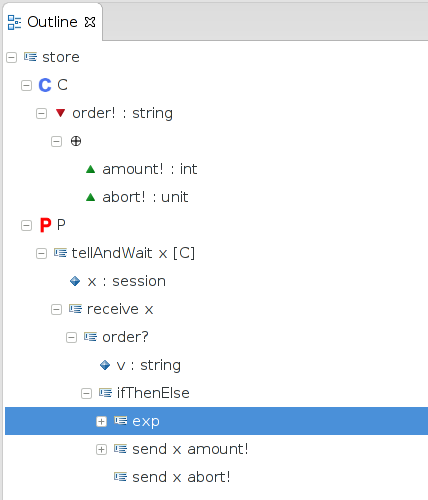
\includegraphics[scale=0.4]{img/outline.png}
\label{fig:outline}
\caption{caption}
\end{figure}
}

\paragraph{Code generation}
The plugin automatically generates corresponding Maude and Java files.
The former can be used directly within Eclipse to verify its honesty,
exploiting the model-checking tool of~\cite{verifiable};
the latter represents a working java skeleton. 
Considering the honest specification describe above, the skeleton looks like
\begin{mdframed}
\begin{minted}[
    fontsize=\scriptsize
    ,linenos
    ]{java}
public class Phonest extends Participant {
            
    public void run() {
        Session<TST> x = tellAndWait(C);    
        Message msg = x.waitForReceive("order");
        
        String v;
        v = msg.getStringValue();
        
        Public<TST> pbl_y = tell(D, 10000);
        try {
            Session<TST> y = pbl_y.waitForSession();
            y.sendIfAllowed("req", v);
            
            try {
                Message msg_1 = y.waitForReceive(10000, "ok", "no");
                
                switch (msg_1.getLabel()) {                    
                    case "ok": x.sendIfAllowed("amount", 100); break;
                    case "no": x.sendIfAllowed("abort"); break;                    
                }
            }
            catch (TimeExpiredException e) {
                parallel(()->{ x.sendIfAllowed("abort"); });
                parallel(()->{ y.waitForReceive("ok", "no"); });
            }            
        }
        catch(ContractExpiredException e) {
            x.sendIfAllowed("abort");
        }
    }
}
\end{minted}
\end{mdframed}

The \inlineCoco{tellRetract} corresponds to perform a tell with
a delay (line \lineno{10}). The successive \code{waitForSession()} blocks until the delay is
expired, throwing a \code{ContractExpiredException} if the session 
was not fused in time (the contract has been retracted).
The timeout \inlineCoco{t} corresponds to a \code{waitForReceived} with a timeout.
The method blocks until a message with label \code{"ok"} or \code{"no"} is received,
or throws a \code{TimeExpiredException} if the timeout expires.

\paragraph{Refining the skeleton}
The order amount is still hardcoded, so we decide to externalize its computation
in a separated method, \eg
\begin{mdframed}
\begin{minted}[
    fontsize=\scriptsize
%    ,linenos
    ]{java}
public int getOrderAmount(String order) {
    File f = new File("/orders/"+order);
    
    try (
            BufferedReader br = new BufferedReader( new FileReader(f) )
            ) {
        String line = br.readLine();
        return Integer.valueOf()[1]);        
    }
    catch (Exception e) {
        throw new RuntimeException(e);
    }
    
}
\end{minted}
\end{mdframed}

\paragraph{Diogenes}
Diogenes allows to verify the honesty of Java programs.
The honesty of a class extending \code{it.unica.co2.api.process.Participant} 
can be verified using the static method \code{HonestyChecker.isHonest(Phonest.class)}.

It returns the enumeration \code{HonestyResult} that can be
\begin{itemize}
\item \code{HONEST}: the tool was able to extract a \coco model and verify that it is honest;
\item \code{DISHONEST}: as above, but the model was dishonest;
\item \code{UNKNOWN}: the tool was unable to extract a model. It can be caused by several issues, such as an error of the tool or unhandled exceptions within the class under test.
\end{itemize}

Consider for example the refinement provided above.

\section{Architecture}

Diogenes has three main components:
an honesty checker for \coco,
an honesty checker for Java,
and an Eclipse plugin which integrates the two analyses
with an editor of \coco.
We illustrate the architecture of our tools in~\Cref{fig:architecture}.

The \coco honesty checker implements the  
verification technique introduced in~\cite{BCPZ15jlamp}.
This technique is built upon an alternative semantics of \coco 
which abstracts both values (sent, received, and in conditional expressions) 
and the actual \emph{context} wherein a process is executed.
This abstraction is a \emph{sound} over-approximation of honesty:
namely, if the abstraction of a process is honest,
then also the concrete one is honest.
Further, in the fragment of \coco without conditional statements
the analysis is also \emph{complete},
\ie if a concrete process is honest, then also its abstraction is honest.
For processes without delimitation/parallel under process definitions,
the associate abstraction is finite-state, 
hence we can verify their honesty by model checking a (finite) state space.
Our implementation 
first translates a \coco process into a Maude term~\cite{Maude01}, 
and then uses the Maude LTL model checker~\cite{Eker02maude}
to decide honesty of its abstract semantics.

%\paragraph{Diogenes.}
The Java honesty checker is developed on top of \emph{Java PathFinder}
(JPF, \cite{lerda2001addressing,visser2003model}).
The JPF core is a Virtual Machine for Java bytecode
that can be configured to act as a model-checker.
It provides the concept of \emph{execution choice}
and \emph{state backtracking}, allowing multiple state exploration.
%
We exploit its capabilities to extract a \coco model
from a Java program. We implement a \emph{listener} that allow us
to catch specific method invocations representing I/O actions
directed to the middleware~\cite{CO2middleware},
and simulate \emph{all} the possible response that 
the application can receive from it.
Once the \coco model is extracted, we verify its honesty
with the model checking technique of~\cite{BCPZ15jlamp}.
Therefore, the analysis strongly depends on the Maude model-checker,
as shown by the data-flow in \Cref{fig:architecture}.
\bartnote{+ commento sulla tecnica di analisi: ad esempio, sotto quali ipotesi e' corretta?}

The Eclipse plugin \bartnote{dire prima cosa fa, e poi dare qualche insight}
% On the contrary, the Eclipse plugin has no dependencies, and
% it integrates the possibility to directly call 
% the Maude model-checker, reporting its output into the Eclipse console.
%
The plugin relies on
Xtext~\cite{xtext-site}, a framework for developing programming languages, 
and Xsemantics~\cite{xsemantics-site}, a domain-specific language for writing type systems
for Xtext-based languages.
%
We use Xtext to define the grammar of \coco.
\bartnote{giusto? si usa per altre cose? c'e' da dire altre cose interessanti sul plugin? mi sembra che questa parte andrebbe espanda un poco}
% We implement an Xtext grammar focusing on~\cite{BCPZ15jlamp},
% and we extend it in order to allow a complete mapping between \coco and Java.


\begin{figure}[t]
    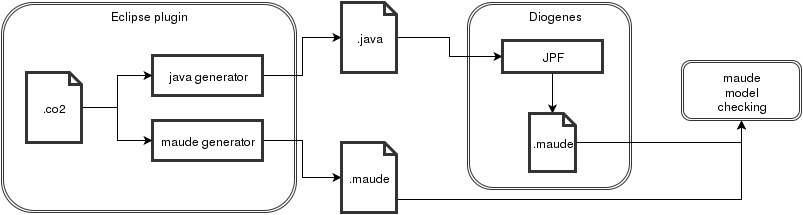
\includegraphics[width=\textwidth]{img/diogenes-arch.png}
    \caption{Data flow schema}
    \label{fig:architecture}
\end{figure}
% \chapter{Use cases}\label{chap:use-cases}

In order to valuate effectiveness of our tools we studied and implemented several use cases. In this chapter we present three of them:

\begin{description}
	\item[Online store:] a store advertise a recursive contract and can interact with buyers one after another (single session). This example, deliberately simple to explain all the verification phases, shows how a \coco specification is translated to Maude and Java, and how the honesty is checked by the Java application.
	
	\item[Voucher distribution system:] this example involve multiple sessions and demonstrate the benefit of our work. First, we provide an honest specification of the process, showing that both Maude and Java programs respond in the same way. Then, we change our specification to be not honest and our verification technique correctly detects the Java program is dishonest.
	
	\item[Blackjack:] the last example shows how a specification can be difficult to write and maintain. The advertised contracts are both recursive and the specification is split into different parts due to its complexity. There are also multiple sessions, parallel processes, if-then-else selection and recursive behaviour.
\end{description}

These examples where extracted from \cite{verifiable} and used as test bench for our implementation\footnote{Please noste that all example below would be rejected by the \coco middleware (\Cref{sec:co2-middleware}) because it does not accept actions whose name does not match \incode{[a-z]+}. This drawback would obligate us to avoid \textit{camelCase}, leading to less readable examples. The solution is to replace all actions with its lowercase.}.

\section{Online store}\label{ex:online-store}
An online store {\pmv A} has the following contract: %
buyers can iteratively add items to the shopping cart (\atom{addToCart});
when at least one item has been added,
the client can proceed to \atom{checkout}.
Then, the client can either \atom{cancel} the order, 
or \atom{pay}.
In the latter case,
the store can accept the payment (\atom{ok}),
or decline it (\atom{no}, in which case it lets the user try again),
or it can \atom{abort} the transaction.
%
Such a contract may be expressed as follows:

\inputCoco{code/co2/online-store/store-contract.co2}

A possible specification of the store is:

\inputCoco{code/co2/online-store/store-process.co2}

The process \inlineCoco{P} first advertises the contract
\inlineCoco{C}, and then waits that the user has performed the
first \atom{addToCart} %
(note that it also requires that the session \inlineCoco{x} is fused with the other participant). %
Then, the store enters a recursive process \inlineCoco{Padd},
wherein it accepts two user choices: \atom{addToCart}, which is
followed by a recursive call to \inlineCoco{Padd}, and
\atom{checkout}, which passes the control to process
\inlineCoco{Ppay}.  In the meanwhile, the overall amount to pay
is accumulated in variable \inlineCoco{total} (we are assuming that the value \inlineCoco{n}
passed by \atom{addToCart} is the price of an item; in more
concrete implementations, such value could be obtained \eg from
product database). %
Within \inlineCoco{Ppay}, after the payment is received, the
store internally chooses (with a rather arbitrary policy) whether to
accept it or not: %
in the first case, it terminates; %
in the second case, it proceeds with \inlineCoco{Ppay}, thus
allowing the user to retry the payment.

\subsection{Maude code}
The process explained in the previous section is automatically translated to two \textit{target} languages, Maude and Java.

The auto-generated Maude code is:
\inputMaude{code/co2/online-store/store-process.maude}

The execution of the above code shows the process \inlineCoco{P} is honest:
\begin{lstlisting}
reduce in STORE : honest(P, ['STORE], 50) .
rewrites: 6852 in 36ms cpu (35ms real) (186871 rewrites/second)
result Bool: true
Bye.
\end{lstlisting}

\subsection{Java code}
In order to translate to Java code, we need to modify our process: the prefix \inlineCoco{tell x C} must be replaced with \inlineCoco{tell x C . ask x}. The \textit{ask} prefix allows us to put the \incodeMethod{waitForSession()}
in the right place.

The auto-generated Java code is contained into one single class, containing a static class for each declared process and a static field for each contract. Username and password, required to interact with the middleware, are also included as static fields.

Contracts are translated as follows:
\inputJava{code/co2/online-store/store-process-contracts.java}

Each contract is declared as \incodeType{ContractWrapper} and set during the class instantiation. Within the plugin, the user can refers to a contract declared later, so we use the wrapper as a workaround, since Java not allow to do this. Recursive contracts, declared within a contract definition, are instantiated as \incodeType{Recursion}. Both contracts type can be set as the next contract of an action.

The process \inlineCoco{P} is translated to:
\inputJava{code/co2/online-store/store-process-P.java}

\inlineCoco{Padd} is translated to:
\inputJava{code/co2/online-store/store-process-Padd.java}

\inlineCoco{Ppay} is translated to:
\inputJava{code/co2/online-store/store-process-Ppay.java}

\inlineCoco{Pack} is translated to:
\inputJava{code/co2/online-store/store-process-Pack.java}


\subsubsection{Honesty}
\incodeType{HonestyChecker.}\incodeMethod{isHonest()} is the static method available to check the honesty. It takes a \incodeType{Class}\generic[Participant]{?} as an argument and print the results to the stream output.

As described in \Cref{sec:construction-phase}, the honesty is checked rebuilding the \coco process and the serializing it as Maude program. The extracted process is:
\inputMaude{code/co2/online-store/store-process-jpf.maude}

As you can see, it is very similar to the Maude process originated by the \coco syntax. The only differences are:
\begin{itemize}
	\item we lose the contract composition
	\item we lose the actions types both in contracts and $\fact{}{}$-prefixes (the middleware does not permit them)
\end{itemize}

The method \incodeType{HonestyChecker.}\incodeMethod{isHonest()} produces
\begin{lstlisting}
-------------------------------------------------- result
honesty: HONEST
==================================================
\end{lstlisting}

\section{Voucher distribution system}
A store {\pmv A} offers buyers two payment options: \cp\ or \cv.
%
If a buyer {\pmv B} chooses \cp, {\pmv A} requires {\pmv B} to \p;
otherwise, {\pmv A} checks the validity of the voucher with {\pmv V}, an
online voucher distribution system.
%
If {\pmv V} validates the voucher (\atom{ok}), {\pmv B} can use it (\vou),
otherwise (\atom{no}) {\pmv B} must \p.

We specify the contracts \inlineCoco{CB} (between {\pmv A} and {\pmv B}) 
and \inlineCoco{CV} (between {\pmv A} and {\pmv V}) 
as follows:
\inputCoco{code/co2/voucher/voucher-contracts.co2}

\subsection{Specification}\label{sec:uses:dishonest-voucher}
A possible specification is specified in~\cite{BTZ12coordination} as follows:
\inputCoco{code/co2/voucher/voucher-process.co2}

Variables \inlineCoco{x} and \inlineCoco{y} in \inlineCoco{P} correspond to two separate
sessions, where {\pmv A} interacts with {\pmv B} and {\pmv V}, respectively.
The advertisement of \inlineCoco{CV} causally depends on the
stipulation of the contract \inlineCoco{CB}, 
because {\pmv A} must fire \inlineCoco{CV} before the rightmost \inlineCoco{tell}.
%
In process \inlineCoco{Q} the store waits for an answer from {\pmv V}:
if {\pmv V} validates the voucher (first branch), 
then {\pmv A} accepts it from {\pmv B};
if {\pmv V} rejects the voucher (second branch), 
then {\pmv A} requires {\pmv B} to pay.
The third branch \inlineCoco{t . R} allows {\pmv A} to reject the voucher.
Here \inlineCoco{t} models a timeout, 
to deal with the fact that \inlineCoco{CV} might either 
not be stipulated, or {\pmv V} might take too long to answer.

This process is not honest \cite{verifiable} and the resulting translation to Maude produces the following output:
\begin{lstlisting}
reduce in VOUCHER : honest(P, ['VOUCHER], 50) .
rewrites: 59554 in 100ms cpu (99ms real) (595540 rewrites/second)
result TSystem: < ($ 0,$ 1)(
    A[do $ 0 "reject" ! unit . do $ 0 "pay" ? string . (0).Sum]
    | $ 0[
        "accept" ! unit . "voucher" ? string . 0
        (+)"reject" ! unit . "pay" ? string . 0] 
    | $ 1[ready "no" ? unit . 0]) >
Bye.
\end{lstlisting}

The lines of the output above show a state where {\pmv A} is not ready:
there, {\pmv A} must do \atom{no} in session \mbox{\code{\$1}}
(which corresponds to variable $y$ in the \coco specification),
while {\pmv A} is only ready to do a \rj\ at session \code{\$0} 
(which corresponds to $x$).
This problem occurs when branch \inlineCoco{t . R} is chosen
(actually, the code within \code{A[...]} is that of \inlineCoco{R}),
so it follows that \inlineCoco{P} is dishonest.
%
To recover honesty, it suffices to replace \inlineCoco{R} with the following process \inlineCoco{R1}, %
where $\pmv{A}$ is ready to handle $\pmv{V}$'s answer when $y$ is fused:

\begin{lstlisting}[language=coco]
process R1 (x:session, y:session){
    (do x reject! . do x pay? code:string)
    | (do y ok? + do y no?)
}
\end{lstlisting}

Now the process \inlineCoco{P} is honest.

\subsection{Honest specification}\label{ex:voucher-honest}
Due to some limitations explained in \Cref{sec:untranslatable-code}, our process is not translatable to Java, so we must introduce an \inlineCoco{ask} for each session.
The modified code is

As you can see, there is not the necessity to the process \inlineCoco{R1} because we handle the timeout separately.

The resulting process (partially refactored) is:
\inputCoco{code/co2/voucher/voucher-process-translatable.co2}

The process is honest as stated by the Maude model checker
\begin{lstlisting}
reduce in VOUCHER : honest(P, ['VOUCHER], 50) .
rewrites: 619654 in 446ms cpu (445ms real) (1387284 
  rewrites/second)
result Bool: true
Bye.
\end{lstlisting}

and from the Java analysis
\begin{lstlisting}
-------------------------------------------------- result
honesty: HONEST
==================================================
\end{lstlisting}

\subsection{Dishonest}\label{ex:voucher-dishonest}
In order to check the validity of out Java analysis, we modify last \inlineCoco{R1} process as follows:

\begin{lstlisting}[language=coco]
process R1 (x:session, y:session){
    abortX(x) //| abortY(y)
}
\end{lstlisting}
The process is dishonest for the same reason explained in \Cref{sec:uses:dishonest-voucher}.
The Maude model checker produces the same output as shown above and in analogous way
our Java analysis print

\begin{lstlisting}
-------------------------------------------------- result
honesty: DISHONEST
==================================================
\end{lstlisting}

Please note that, as described in \Cref{sec:verification-phase}, the check of the honesty of a Java program is made building a \coco process, serialized as Maude program and finally model-checked as described \Cref{sec:maude:checker}. For this reason, we not print the system configuration where the process is dishonest because is available as plain string (the output of the model-checker) and would not be useful to an user not experienced with the Maude model-checker.

\section{Blackjack}\label{ex:blackjack}
We model an online blackjack server, using simplified casino rules.
The game involves two players: {\pmv P} (for player) and {\pmv A} (for \emph{dealer}).
The goal of {\pmv P} is to beat the dealer, 
by accumulating a hand of cards whose value is greater than that of the dealer;
furthermore, the value of the hand must not exceed $21$.
The game has two turns: first the player turn, and then the dealer turn.
In the player turn, {\pmv A} deals cards to the player;
after a card is received, the player can decide whether to get another one
(\atom{hit}) or to terminate his turn (\atom{stand}).
In the dealer turn, {\pmv A} deals cards for himself, with the goal
of obtaining a hand with value greater than the player's hand.
The player (possibly, {\pmv A}) which exceeds $21$ loses the game.

The contract \inlineCoco{Cp} advertised by the dealer to players is the following:

\inputCoco{code/co2/blackjack/player-contract.co2}

Players can choose between taking a card (\atom{hit}) or 
passing the turn (\atom{stand}).
In the first case, the dealer either gives a \atom{card} to the player
(and returns to the beginning of the contract),
or it notifies that the player \atom{lose}s
(or it may \atom{abort} the game).
In the second case (\atom{stand}), the dealer 
notifies to the player if he has won or lost 
(or if the game has been aborted).

To implement the game, the dealer resorts to an external service
which provides the features of a deck of cards.
The contract between the dealer and the deck of cards is 
formalised by \inlineCoco{Cd} as follows:
\inputCoco{code/co2/blackjack/dealer-contract.co2}

The dealer can recursively 
ask for a new card (\atom{next}) and receive it (\atom{card})
as an integer value,
or it may \atom{abort} the interaction with the deck of cards service.

We specify the dealer as the following process \inlineCoco{P}:
\inputCoco{code/co2/blackjack/process-P.co2}

The first \inlineCoco{tell xd} advertises the contract for the
deck of cards.
The dealer waits (via the \inlineCoco{ask xd} prefix) that such contract
is fused, 
and then it advertises the contract for the player 
(with the second \inlineCoco{tell xp}). Next, it waits for a session with
the dealer (via the \inlineCoco{ask xd}) and passing the control to \inlineCoco{Pplay}.
The prefix \inlineCoco{t} models a timeout, where the dealer stops the interaction with the deck service and handle a session with a possible player (via \inlineCoco{PabortP}).

At this point the control is passed to the process
\inlineCoco{Pplay}, which is specified as follows:

\inputCoco{code/co2/blackjack/process-Pplay.co2}

Process \inlineCoco{Pplay} waits for a player decision.
If the player chooses \atom{hit} 
then the dealer asks the deck for the next card,
and the control passes to \inlineCoco{Pdeck}.
Instead, if the player chooses \atom{stand},
the control passes to \inlineCoco{Qstand}.
The third branch models a timeout, 
where the dealer stops waiting for the player decision, 
and it just aborts all the sessions.
The parameter \inlineCoco{np} is used to accumulate the value of the player hand
(\ie, the summation of the value of the cards he has received).

\inputCoco{code/co2/blackjack/process-Pdeck.co2}

Process \inlineCoco{Pdeck} waits for the value $n$ of the card
provided by the deck, and then passes the control to \inlineCoco{Pcard}.
Also in this case, a timeout branch ensures that sessions are aborted
in case the deck does not reply timely.

\inputCoco{code/co2/blackjack/process-Pcard.co2}

Process \inlineCoco{Pcard} checks whether the player hand exceeds $21$:
if so, it tells the player that he has lost; 
otherwise, the player is allowed to take another turn.

\inputCoco{code/co2/blackjack/process-Qstand.co2}

Process \inlineCoco{Qstand} is invoked upon the player
has decided to stand.
The dealer checks that the value \inlineCoco{nd} of its hand 
(initially set to $0$) is less then $21$.
If so, the dealer asks the deck for the next card,
and the control passes to \inlineCoco{Qdeck};
otherwise, it tells the player that he has won.

\inputCoco{code/co2/blackjack/process-Qdeck.co2}

Process \inlineCoco{Qdeck} waits for the card, and then proceeds
to \inlineCoco{Qcard}
(as above, also in this case we use a timeout branch to avoid deadlock).

\inputCoco{code/co2/blackjack/process-Qcard.co2}

Process \inlineCoco{Qcard} compares the hand \inlineCoco{np} of the player 
with that \inlineCoco{nd} of the dealer. 
If the dealer hand has not reached \inlineCoco{np}, the dealer takes another card;
otherwise, the player has lost.

\inputCoco{code/co2/blackjack/process-PabortP.co2}
\inputCoco{code/co2/blackjack/process-PabortD.co2}

Finally, processes \inlineCoco{PabortP} and \inlineCoco{PabortD} 
ensure that the sessions with the player and with the deck of cards,
respectively, are aborted correctly.

Both generated processes (Maude and Java) results to honest.

\section{Benchmarks}
To empirically valuate the effectiveness of our verification technique,
we have applied the Maude honesty checker on all the case studies 
presented above.

The experiments have measured, for each case study, 
the average construction of \coco process from Java code,
the average time of model checking (Maude) and the average completion time. %
The testing environment is a PC with an Intel Core i7-4790K CPU @ 4.00GHz 
and 32G of RAM, running Ubuntu 14.04. %
The results are reported in~\Cref{tab:benchmarks}.


\begin{table}[t]
	\center
	\footnotesize
	\begin{tabular}{|c|c|ccc|}
		\hline
		&  & \textbf{Build} & \textbf{Model check} & \textbf{Total}  \\
		\textbf{Example}& \textbf{Ref.}	&	\textbf{avg. time}	&	\textbf{avg. time}	&	\textbf{avg. time} \\
		&	&	(ms)		&	(ms)		&	(ms) \\
		\hline
		\hline
		Online store					& \Cref{ex:online-store} 		& 108 	& 80 	& 188 \\
		\hline
		Voucher dist. sys (honest) 		& \Cref{ex:voucher-honest} 		& 135 	& 183 	& 318 \\
		\hline
		Voucher dist. sys (dishonest) 	& \Cref{ex:voucher-dishonest} 	& 100 	& 192 	& 293 \\
		\hline
		Blackjack 						& \Cref{ex:blackjack} 			& 249 	& 247	& 497 \\
		\hline
	\end{tabular}
	\caption{Benchmarks for the Java honesty checker.}
	\label{tab:benchmarks}
\end{table}

%--------------------------------
%------------ Stats ------------
%--------------------------------
%Process: it.unica.co2.examples.plugin.Blackjack$P
%JPF:    249
%Maude:    247
%Total:    497
%--------------------------------
%Process: it.unica.co2.examples.plugin.OnlineStore$P
%JPF:    108
%Maude:    80
%Total:    188
%--------------------------------
%Process: it.unica.co2.examples.plugin.VoucherHonest$P
%JPF:    135
%Maude:    183
%Total:    318
%--------------------------------
%Process: it.unica.co2.examples.plugin.VoucherDishonest$P
%JPF:    100
%Maude:    192
%Total:    293
%--------------------------------
\section{Conclusion}

\subsection{Limitations}
- time constrains

- action types

\subsection{Future works}

\paragraph{Eclipse plugin}
- graphical editor (You can combine the text-based formats created with Xtext with many graphical editing frameworks, e.g. Sirius or Graphiti. Xtext offers this flexibility by supporting EMF as common data layer. An Xtext language can be used as storage format for another primary editor, and you can even embed text editors inside a graphical editor.)

\paragraph{Diogenes}


%
\section{Background}\label{sec:background}


\subsection{Session types and compliance}
A contract describes the intended behaviour of \emph{one} of the two
participants involved in a session.  We use binary session
types~\cite{Honda98esop} to define contracts.  Session types are terms
of a process algebra featuring internal/external choice, and
recursion.

We assume a set of \emph{participants} (ranged over by
${\pmv A}, {\pmv B}, \ldots$), a set of \emph{branch labels} (ranged
over by $\atom{a}, \atom{b}, \ldots$), and a set of \emph{sorts}
ranged over by $\sortT, \sortTi, \ldots$ (e.g.\ \sort{int},
\sort{bool}, \sort{unit}).  Each sort $\sort{T}$ is populated by a set
of values, ranged over by $\valV, \valVi, \ldots$; as usual, we write
$\valV: \sortT$ to indicate that $\valV$ has sort~$\sortT$.

\begin{definition}[Contracts] \label{def:contracts:syntax}
Contracts are \emph{binary session types}, i.e.\ terms defined by the grammar:
\begin{align*}
%\text{Unilateral contracts} &&
    \contrP,\contrQ \;\; & ::= \;\;
    % \textstyle
    \SumInt[i \in \mathcal{I}]{\atomOut[i]{a} \sortT[i]}{\contrP[i]} \ \bnfmid \ 
    \SumExt[i \in \mathcal{I}]{\atomIn[i]{a} \sortT[i]}{\contrP[i]} \ \bnfmid \
    % \ready{\atomIn{a}\val{v}}.c \ \bnfmid \
    \rec{\contrX}{\contrP}
    \bnfmid \ \contrX
\end{align*}
where % we assume that
\begin{inlinelist} 
\item the index set $\mathcal{I}$ is finite,
\item \label{item:def:contracts:syntax:pairwise-distinct}
the labels $\atom[i]{a}$ in the prefixes of each summation are pairwise distinct, and 
\item recursion variables $\contrX$ are prefix-guarded.
\end{inlinelist}
\end{definition}

An internal sum $\SumInt[i]{\atomOut[i]{a}\sortT[i]}{\contrP[i]}$
allows a participant to choose one of the labels $\atom[i]{a}$, to
pass a value of sort $\sortT[i]$, and then to behave according to the
branch $\contrP[i]$.  Dually, an external sum
$\SumExt[i]{\atomIn[i]{a}\sortT[i]}{\contrP[i]}$ allows to wait for
the other participant to choose one of the labels $\atom[i]{a}$, and
then to receive a value of sort $\sortT[i]$ and behave according to
the branch $\contrP[i]$.
%
Empty internal/external sums are identified, and they are denoted with
$\cnil$, which represents a \emph{success state} wherein the
interaction has terminated.

%We use the (commutative and associative) binary operators to isolate a
%branch in a sum: \eg,\
%$\contrP = (\sumI{\atomOut{a}\sortT}{\contrPi}) \sumInt \contrPii$
%means that $\contrP$ has the form
%$\SumInt[i \in \mathcal{I}]{\atomOut[i]{a}\sortT[i]}{\contrP[i]}$ and
%there exists some $i \in \mathcal{I}$ such that
%$\sumI{\atomOut{a}\sortT}{\contrPi} =
%\sumI{\atomOut[i]{a}\sortT[i]}{\contrP[i]}$.
%Hereafter, we will omit the $\sort{unit}$ sort and the trailing
%occurrences of $\cnil$, and we will only consider contracts without
%free occurrences of recursion variables~$\contrX$.

To model the behaviour of two participants {\pmv A} and {\pmv B}
involved in a session, we compose their contracts together into
$\bic{\contrP}{\contrQ}$.  Their interaction is ruled by an
operational semantics \tizinote{citare} \Cref{citare}, where the two
participants alternate in firing actions: in partcular {\pmv A} can
fire either if she has an internal choice, or if she is committed to a
branch of an external choice.
%
To do that, the syntax of~\Cref{def:contracts:syntax} has been
extended with the term $\ready{\atomIn{a}\val{v}} \contrSeq
\contrP$,
which models a participant ready to input a value $\valV$ in a branch
with label $\atom{a}$, and then to continue as $\contrP$.  In other
words, $\ready{\atomIn{a}\val{v}}$ acts as a one-position buffer
shared between the two participants.

%
%
Two composed contracts may enjoy the property of
\emph{compliance}. The intuition is that if a contract $\contrP$ is
compliant with a contract $\contrQ$, then in all the configurations of
a computation of $\bic{\contrP}{\contrQ}$, whenever a participant
wants to choose a branch in an internal sum, the other participant
always offers the opportunity to do it.  Compliance guarantees
that % \emph{progress}:
whenever a computation of %$\bic{\contrP}{\contrQ}$ 
becomes stuck, then
both participants have reached the success state $\cnil$.


\subsection{The \coco calculus and honesty}\label{sec:co2}

We model agents and systems in the process calculus 
\coco\cite{BZ10lics,BTZ12coordination,BSTZ13forte},
which we instantiate with the contracts introduced in \Cref{sec:contract-session-types}.

Let $\vars$ and $\snames$ be disjoint sets
of \emph{variables} (ranged over by $x,y,\ldots$) and 
\emph{names} (ranged over by $s,t,\ldots$).
%
We assume a language of \emph{expressions}
(ranged over by $\expE, \expEi, \ldots$),
containing variables, values, and operators 
(\eg the usual arithmetic/logic ones).
The actual choice of operators is almost immaterial for the
subsequent technical development; here we just postulate
a function $\sem{\cdot}$ which maps (closed) expressions to values.
We assume that the sort of an expression is uniquely determined 
by the sorts of its variables.
We use $u,v,\ldots$ to range over $\vars \cup \snames$,
we use $\vec{u},\vec{v},\ldots$ to range over 
sequences of variables/names, and
$\vec{e}$ to range over sequences of expressions.
To make symbols lookup easier, we have summarised the syntactic categories 
and some notation in Table~\ref{def:notation}.
% Some of the symbols defined therein will only be used in later sections.

% \begin{table}[t]
% 	\footnotesize
% 	\hrulefill
% 	% \vspace{-10pt}
% 	\[
% 	\begin{array}{ll}
	
% 	\begin{array}{ll}
% 	\pmv{A}, \pmv{B}, \ldots & \text{Participant names}
% 	\\
% 	\atom{a}, \atom{b}, \ldots & \text{Branch labels}
% 	\\
% 	\sortT, \sortTi, \ldots & \text{Sorts}
% 	\\
% 	\valV, \valVi, \ldots & \text{Values}
% 	\\
% 	\contrP, \contrQ, \ldots & \text{Contracts}
% 	\\
% 	\gamma, \gammai, \ldots & \text{Contract configurations} 
% 	\\
% 	%   \contrP \compliant \contrQ & \text{Compliance}
% 	%   \\
% 	%   \cfrown{\pmv A}{\gamma} & \text{Culpability}
% 	%   \\
% 	\gamma \cmove{} \gammai & \text{Transition of contracts}
% 	\end{array}
	
% 	& \hspace{18pt}
	
% 	\begin{array}{ll}
% 	u, v,\ldots \mbox{\hspace{50pt}} & \text{Union of:} 
% 	\\
% 	s,t, \ldots \in \snames & \text{Session names} 
% 	\\
% 	x, y, \ldots \in \vars & \text{Variables} 
% 	\\
% 	\expE, \expEi, \ldots & \text{Expressions} 
% 	\\
% 	\procP,\procQ,\ldots & \text{Processes} 
% 	\\
% 	\sysS, \sysSi,\ldots & \text{Systems}
% 	\\
% 	%   \vabscontrP, \vabssysS, \ldots & \text{Value-abstract contracts/systems}
% 	%   \\
% 	%   \cabscontrP, \abssysS, \ldots & \text{Context-abstract contracts/systems}
% 	%   \\
% 	\sysS \pmove{} \sysSi & \text{Transition of systems}
% 	\end{array}
	
% 	\end{array}
% 	\]
% 	\hrulefill
% 	\vspace{-5pt}
% 	\caption{Summary of notation.} \label{def:notation}
% \end{table}


\begin{definition}\label{def:co2:syntax}
	The syntax of \coco is defined as follows:
	\[
	\small
	\begin{array}{r@{\hskip 0.1cm}lclcccccccccccc}   
	& \sysS \, (\text{Systems}) & ::= & 
	\emptysys 
	~\bnfmid ~ \sys {\pmv A} \procP 
	\; \bnfmid \; \sys s \gamma 
	\; \bnfmid \; (u)\sysS
	\; \bnfmid \; \sysS \mid \sysS
	\; \bnfmid \; \setenum{\freeze u \contrP}_{\pmv A}
	\\[.8pc]
	
	& \procP \, (\text{Processes})& ::= &  \textstyle 
	\cocoSum[i]{\pref[i] \cocoSeq \procP[\!i]}
	\; \bnfmid \; \ifte{\expE}{\procP}{\procP}
	\; \bnfmid \; \procX(\vec u,\vec e)
	\; \bnfmid \; (u)\procP
	\; \bnfmid \; \procP \cocoPar \procP
	\\[.8pc]
	
	& \pref \, (\text{Prefixes})& ::= & \tau
	\; \bnfmid \; \tell {} {\freeze u \contrP}
	\; \bnfmid \; \fact u {\atomOut{a} e}
	\; \bnfmid \; \fact u {\atomIn{a} x : \sortT}
	\; \bnfmid \; \ask {u} {\!\phi}
	\end{array}
	\]
	If $\vec u = u_0,\hdots,u_n$,
	we will use $(\vec u) \sysS$ and $(\vec u) \procP$ 
	as shorthands for $(u_0)\cdots(u_n) \sysS$ and $(u_0)\cdots(u_n) \procP$,
	respectively. %
	We also assume the following syntactic constraints on processes and systems:
	\begin{enumerate}
		
		\item each occurrence of named processes is prefix-guarded;
		
		\item in $(\vec u)(\sys {\pmv A} \procP \mid \sys{\pmv B} \procQ \mid \cdots)$,
		it must be $\pmv A \neq \pmv B$;
		
		\item in $(\vec u)(\sys s \gamma \mid \sys t \gammai \mid \cdots)$,
		it must be $s \neq t$.
		
	\end{enumerate}
\end{definition}


\begin{figure}[t]
	\hrulefill
	\footnotesize
	\begin{center}
		commutative monoidal laws for $\mid$ on processes and systems
	\end{center}
	\vspace{-10pt}
	\[
	\begin{array}{c}
	\sys {\pmv A} {(v) \procP} \equiv \sys{(v) \, {\pmv A}} \procP 
	\hspace{20pt}
	\sysFmt{Z} \mid (u) \sysFmt{Z'} \equiv (u)(\sysFmt{Z} \mid \sysFmt{Z'}) 
	\;\;\text{if}\ u \not\in \fv{\sysFmt{Z}} \cup \fn{\sysFmt{Z}}
	\\[8pt]
	(u)(v) \sysFmt{Z} \equiv (v)(u) \sysFmt{Z}
	\hspace{20pt}
	(u) \sysFmt{Z} \equiv \sysFmt{Z}
	\;\;\text{if}\ u \not\in \fv{\sysFmt{Z}} \cup \fn{\sysFmt{Z}}
	\hspace{20pt} 
	\setenum{\freeze s \contrP}_{\pmv A} \equiv \pnil 
	\end{array}
	\]
	\hrulefill
	\vspace{-5pt}
	\caption[Structural equivalence for \coco]{Structural equivalence for \coco 
		($\sysFmt{Z},\sysFmt{Z'}$ range over systems or processes).} \label{fig:co2:equiv}
	\vspace{-10pt}
\end{figure}


\emph{Systems} $\sysS, \sysSi,\ldots$ are the parallel composition of 
\emph{participants} $\sys {\pmv A} \procP$,
\emph{sessions} $\sys s \gamma$,
\emph{delimited systems} $(u)\sysS$, 
and \emph{latent contracts} $\setenum{\freeze{u\!\!}{\contrP}}_{\pmv A}$.
A latent contract $\setenum{\freeze{x\!\!}{\contrP}}_{\pmv A}$ 
represents a contract $\contrP$ (advertised by {\pmv A}) which
has not been stipulated yet; upon stipulation, the variable $x$ will be
instantiated to a fresh session name. 
% Latent contracts of the form 
% $\setenum{{\freeze s c}_{\pmv A}}$, where $s$ is a session \emph{name} are discarded
% by the axiom $\setenum{{\freeze s c}_{\pmv A}} \equiv \pnil$ in~\Cref{fig:co2:equiv}.

\emph{Processes} $\procP, \procQ, \ldots$ are
prefix-guarded (finite) sums of processes,
conditionals $\ifte{\expE}{\procP}{\procQ}$
(where $\expE$ is a boolean valued expression),
named processes $\procX(\vec u,\vec e)$ %
(used \eg\ to specify recursive behaviours),
delimited processes $(u) \procP$,
and parallel compositions $\procP \cocoPar \procP$.

\emph{Prefixes} $\pref$ include silent action $\tau$, 
contract advertisement $\tell{}{\freeze u \contrP}$, 
output action $\fact{u}{\atomOut{a}\expE}$,
input action $\fact{u}{\atomIn{a}x:\sortT}$,
and contract query $\ask{u}{\phi}$
(where $\phi$ is an LTL formula on $\gamma$).
%
In each prefix $\pref \neq \tau$, 
the index $u$ refers to the target session involved in
the execution of $\pref$.

\smallskip
The only binder for names is the
delimitation $(u)$, both in systems and processes.
Instead, variables have two binders:
delimitations $(x)$ (both in systems and processes),
and input actions.
Namely, in a process $\fact u {\atomIn{a}x}:\sortT.\, \procP$, 
the variable $x$ in the prefix binds the occurrences of $x$ within $\procP$.
Note that ``value-kinded'' variables in input actions 
will be replaced by values,
while ``name-kinded'' variables used in delimitations 
will be replaced by session names.
Accordingly, we avoid confusion between these two kinds of variables.
For instance, we forbid
$\fact{u}{\atomIn{a}x}.\, \fact{x}{\atomOut{b}{\valV}}$
and
$(x) \, \fact{u}{\atomOut{a}{x}}$.
%
% We assume that the variables used in input actions are disjoint from 
% those used in delimitations.

Free \emph{session} names/variables in a prefix are defined as follows:
$\fnv{\tau} = \emptyset$, and
\(
\fnv{\tell{}{\freeze u \contrP}} = 
\setenum{u} = 
\fnv{\fact u {\atomOut a}\expE} =
\fnv{\fact u {\atomIn a}x:\sortT}
\).
Free variables/names of systems/processes are defined accordingly, 
and they are denoted by $\fv{}$ and $\fn{}$.
A system or a process is \emph{closed} when it has no free variables.

We write $\pref[1] \cocoSeq \procP[1] \cocoPlus \pref[2] \cocoSeq
\procP[2]$ for $\cocoSum[{i \in \setenum{1,2}}] {\pref[i]} \cocoSeq
\procP[i]$, and $\pnil$ for $\cocoSum[{\emptyset}]\procP$.
%
We stipulate that each process identifier $\procX$ 
has a unique defining equation
$\procX(x_1, \ldots, x_j) \mmdef \procP$ such that $\fv{\procP} \subseteq
\setenum{x_1,\ldots,x_j} \subseteq \vars$.
We will sometimes omit %
the arguments of $\procX(\vec u, \vec e)$ when they are clear from the context.
As usual, we omit trailing occurrences of~$\pnil$ in processes.

We call  \emph{obligations} those actions a participant $\pmv A$ at a
session $s$ in $\sysS$ has to fire.  
%
A \coco process is \emph{honest} if, in all possible interactions, it
always fulfils its contractual obligations.  

We now address the problem of automatically verifying honesty.
However, this is a desirable goal, 
because it alerts system designers before they
deploy services which could violate contracts at run-time 
(so possibly incurring in sanctions).
%
Verifying honesty in \coco is undecidable in
general~\cite{BTZ12coordination}, because one must consider \emph{all}
possible execution contexts, which are infinite.  Even with usual
syntactic restrictions required to make processes finite-state (\eg\
no delimitation/parallel under process definitions) value-passing
makes the semantics of \coco infinite-state.

Even thought, adopting the aforementioned restrictions and with an abstraction
to approximate values, a checker for honesty has been  implemented
in Maude \cite{Maude01} and described in details in \cite{verifiable}.


\subsection{Contract oriented middleware}
The following section briefly describe a \textit{contract-oriented
  middleware} \cite{CO2middleware} that aims to monitor the
interaction between mutually distrusting services and simplify the
development of distributed applications.  A service can
\textit{advertise} its contract without worrying about the search of a
\textit{compliant} peer to interact with. The middleware carry about
the creation of a session and monitors the involved services to detect
contract violations.

In order to interact with the middleware, a developer can choose
between the RESTFUL API, whose drawback is warring of the order of API
calls, and language specific API, that partially guide it to the
correct usage. At the time of writing, there is a Java API we used in
our implementation (see \Cref{chap:co2-to-java} and
\Cref{chap:java-honesty}).

\subsection{Java API}\label{sec:co2-middleware-api}

%\begin{listing}[t]
%	\inputJavaLineos{code/HelloWorld.txt}
%	\caption{Hello world.}
%	\label{lst:hello-world}
%\end{listing}

This section shows the Java API usage \textit{by example}. 

\Cref{lst:hello-world} shows a simple ``hello world'' example. %
At lines~\lineno{1-2} the process establishes 
a connection with the middleware. %
% In our first example we focus on the basic client APIs that allow to: build a new contract,
% wait for a compliant one, handle a session.
The contract (constructed at line~\lineno{4}) advertise that the
process wants to send a $\atom{greet}$ing message, and waits to
receive the name of the greeted planet.

At line~\lineno{6}, we construct a \incodeType{Private} object, in a
state where it has not been advertised to the middleware, yet. %
As soon as it is advertised by invoking the \incodeMethod{tell} method
at line~\lineno{7}, its state is changed into \incodeType{Public}.  At
line~\lineno{9}, it waits for a session to be established; so that a
\incodeType{Session} object is created, through which the process can
interact with the participant at the other endpoint.  At
line~\lineno{10}, it says \incode{hello}, by sending a message with
label $\atom{greet}$. %
%
At line~\lineno{13}, it waits to receive a \incodeType{Message}. %
If the other participant respects its contract,
\incodeMethod{getStringValue} at line~\lineno{14} 
gets the string associated to the $\atom{planet}$ action,
and the session terminates successfully. %
Otherwise, the \incodeMethod{waitForReceive} is unblocked,
and a \incodeType{ContractException} is caught at line~\lineno{12}.

You can download the Java API, the related documentation and some
examples at ????%\citeurl{CO2middleware} (visited on 2015-08).

\subsubsection{Contract advertisement}
The API allows us to advertise a contract only as plain Java
\incodeType{String} in two formats: XML and \textit{timed
  session-types} \cite{Bartoletti15forte}. The former is too verbose
and does not strictly comply our session-types definition (see
\Cref{def:contracts:syntax}); the latter is a superset of our
specification, so we prefer to use it on communicating with the
middleware.

In \Cref{chap:co2-to-java} we show an extended version of these API,
providing a Java representation for contracts.


% 
\chapter{Eclipse plugin development}\label{chap:eclipse-pde}

A part of this master thesis is the development of an Eclipse plugin that will help the \coco users to write their own processes taking advantage of basic feature such as syntax highlighting, content assist, validation, types check an so on. In order to do so, we discovered \emph{Xtext} \cite{xtext-site}, a framework for development of domain specific languages (DSL) developed in the Eclipse Project as part of the Eclipse Modeling Framework Project, and \emph{Xsemantics} \cite{xsemantics-site}, a tool for writing type systems, reduction rules, interpreters (and in general relation rules) for languages implemented in Xtext.

This chapter provides the basic notions required to understand the implementative part of the thesis: in \Cref{sec:eclipse-overview} we provide an overview of the Eclipse platform and its plugin mechanism (mainly extracted from the Eclipse official documentation \cite{eclipse-official}), then we focus on Xtext and Xsemantics showing their the main aspects, respectively in \Cref{sec:xtext} and \Cref{sec:xsematics}. 

\section{Eclipse overview}\label{sec:eclipse-overview}
The Eclipse platform is structured around the concept of plug-ins. Plug-ins are structured bundles of code and/or data that contribute functionality to the system. Functionality can be contributed in the form of code libraries (Java classes with public API), platform extensions, or even documentation. Plug-ins can define extension points, well-defined places where other plug-ins can add functionality.

Each subsystem in the platform is itself structured as a set of plug-ins that implement some key function. Some plug-ins add visible features to the platform using the extension model. Others supply class libraries that can be used to implement system extensions.

The Eclipse SDK includes the basic platform plus two major tools that are useful for plug-in development.  The Java development tools (JDT) implement a full featured Java development environment.  The Plug-in Developer Environment (PDE) adds specialized tools that streamline the development of plug-ins and extensions.

These tools not only serve a useful purpose, but also provide a great example of how new tools can be added to the platform by building plug-ins that extend the system. Figure \ref{img:eclipse-sdk} show the basic architectural schema.

\begin{figure}
\centering
\includegraphics[scale=0.6]{img/eclipse-sdk-arch}
\caption[The Eclipse SDK architecture]{The Eclipse SDK architecture.}
\label{img:eclipse-sdk}
\end{figure}

\subsection{Runtime core}
The platform runtime engine is started when a user starts an application developed with Eclipse. The runtime implements the basic plug-in model and infrastructure used by the platform. It keeps track of all installed plug-ins and the functionality that they provide.

A plug-in is a structured component that contributes code (or documentation or both) to the system and describes it in a structured way. Plug-ins can define \emph{extension points}, well-defined function points that can be extended by other plug-ins. When a plug-in contributes an implementation for an extension point, we say that it adds an \emph{extension} to the platform. These extensions and extension points are declared in the plug-ins's manifest (\emph{plugin.xml}) file.

Using a common extension model provides a structured way for plug-ins to describe the ways they can be extended, and for client plug-ins to describe the extensions they supply. Defining an extension point is much like defining any other API. The only difference is that the extension point is declared using XML instead of a code signature. Likewise, a client plug-in uses XML to describe its specific extension to the system.

A general goal of the runtime is that the end user should not pay a memory or performance penalty for plug-ins that are installed, but not used. The declarative nature of the platform extension model allows the runtime engine to determine what extension points and extensions are supplied by a plug-in without ever running it. Thus, many plug-ins can be installed, but none will be activated until a function provided by a plug-in has been requested according to the user's activity. This is an important feature in providing a scalable, robust platform. 

\subsection{Plugin mechanism}
The mechanics for supporting plug-ins are implemented using the OSGi framework \cite{osgi-site}. What is OSGi? The best definition is given by the official site:

\begin{displayquote}
\emph{OSGi technology is a set of specifications that defines a dynamic component system for Java. These specifications reduce software complexity by providing a modular architecture for large-scale distributed systems as well as small, embedded applications.} 
\end{displayquote}

Eclipse Equinox \cite{equinox-site} is an implementation of the OSGi core framework specification, a set of bundles that implement various optional OSGi services and other infrastructure for running OSGi-based systems. The Equinox OSGi core framework implementation is used as the reference implementation and as such it implements all the required features of the latest OSGi core framework specification.

Luckily we do not need to delve further in this direction. Exploiting the modularity nature of Eclipse, our attention focused on Xtext and its extensions points. \Cref{sec:xtext} describe its main features and \Cref{sec:co2-plugin} present how we create the \coco plugin.

\section{Xtext: framework for DSL development}\label{sec:xtext}
Xtext is a framework for development of programming languages and \textit{Domain Specific Languages} (DSL) \cite{xtext-site}. The implementation of a DSL take into account not only the language itself but also all the tools you must provide to the end-users (who effectively will use your language), i.e. an editor with syntax highlighting, parsing error and semantic validation.

Xtext provides us with a set of domain-specific languages\footnote{Xbase is a partial programming language implemented in Xtext and is meant to be embedded and extended within other programming languages and DSL written in Xtext.} and modern APIs to describe the different aspects of our programming language. They include such things as the parser, the type-safe abstract syntax tree (AST), the serializer and code formatter, the scoping framework and the linking, compiler checks and static analysis aka validation and a code generator or interpreter. It is also possible to add custom implemetation to the default scoping system and implement custom validation rules that depends on the semantic of our \coco language (i.e. we do not permit to write a contract sum with a repeated action).

\subsection{Xtend}
Xtext strongly encourages you to use Xtend, a statically-typed programming language which translates to comprehensible Java source code. It improves the Java language, \ie introducing lambda expressions, extension methods, operator overloading, multiple dispatch, and so on. Since it compiles to Java code (not Bytecode), Xtend has zero interoperability issues with Java and it is only much more concise, readable and expressive than Java \cite{xtend-site}. We use it to implement all the customization needed by our language.

\subsection{Grammar definition}
Xtext provides a DSL designed for the description of textual languages. The main idea is to describe the concrete syntax and how it is mapped to an in-memory representation. This model will be produced by the parser when it consumes an input file. This model is not a simple \textit{Abstract Syntax Tree} (AST) but a graph of objects with cross-references that can be explored for adding custom validation rules or scoping behaviour.

After you write the grammar, Xtext generate the parser for your language using ANTLR (Another Tool for Language Recognition) which implements a LL(*) parser \cite{antlr-site}. Furthermore, it creates all the scaffolding classes you can use to extend the default features.

\subsection{Code generation}
Xtext provides the notion of \textit{generator} to translate/compile our language to any target language.
From the exploration of the AST, it's possible to implement multiple generators to obtain an executable program. This feature is exploited to compile the \coco language to Java and Maude\cite{Maude01}: the former provides a real implementation of a contract-oriented application, while the former can be exploited to model-check the honesty of the \coco specification, as explained in \Cref{sec:co2-model-check}. This aspects are shown in \Cref{chap:co2-to-java} and \Cref{chap:use-cases}.

\section{Xsemantics}\label{sec:xsematics}
A \emph{type-system} is a collection of rules that assigns a property (called \emph{type}) to various constructs a computer program consists of, such as \emph{variables}, \emph{expressions} or \emph{functions}. The main purpose of a type system is to reduce possibilities for bugs in computer programs checking that the parts have been connected in a consistent way. This checking can happen statically (at compile time), dynamically (at run time), or as a combination of static and dynamic checking.

We provide a static type-system exploiting Xsemantics\cite{xsemantics-site}, a DSL (implemented in Xtext itself) for writing type systems, reduction rules, interpreters (and in general relation rules) for languages implemented in Xtext.

In Xsemantics, The type-system rules are a set of \emph{judgment rules} which have a conclusion and a set of premises; these rules can act on any Java object, though, typically, they will act on the AST derived by our language (implemented with Xtext).
% 
\chapter{Model checking Java programs}\label{chap:model-java}

Model-checking is a technique that allows to verify if a software program satisfies certain properties in \emph{all possible states}.
\Cref{sec:model-checking} describes some basic notions of model-checking, mainly extracted from \cite{baier2008principles}, while \Cref{sec:jpf} shows Java PathFinder, a Java model-checker.

\section{Model checking}\label{sec:model-checking}
In software and hardware design of complex systems, more time and effort are spent on
verification than on construction. Techniques are sought to reduce and ease the verification efforts while increasing their coverage. Formal methods offer a large potential to obtain an early integration of verification in the design process, to provide more effective verification techniques, and to reduce the verification time.

During the last two decades, research in formal methods has led to the development of
some very promising verification techniques that facilitate the early detection of defects. These techniques are accompanied by powerful software tools that can be used to automate various verification steps.

Model checking is a verification technique that explores all possible system states in a brute-force manner.  Similar to a computer chess program that checks possible moves, a model checker, the software tool that performs the model checking, examines all possible system scenarios in a systematic manner. In this way, it can be shown that a given system model truly satisfies a certain property. It is a real challenge to examine the largest possible state spaces that can be treated with current means, i.e., processors and memories. State-of-the-art model checkers can handle state spaces of about $10^8$ to $10^9$ states with explicit state-space enumeration. Using clever algorithms and tailored data structures, larger state spaces ($10^{20}$ up to even $10^{476}$ states) can be handled for specific problems. Even the subtle
errors that remain undiscovered using emulation, testing and simulation can potentially be revealed using model checking.

Typical properties that can be checked using model checking are of a qualitative nature: Is the generated result OK?, Can the system reach a deadlock situation, e.g., when two concurrent programs are waiting for each other and thus halting the entire system?  But also timing properties can be checked: Can a deadlock occur within 1 hour after a system reset?, or, Is a response always received within 8 minutes?  Model checking requires a precise and unambiguous statement of the properties to be examined.  As with making an accurate system model, this step often leads to the discovery of several ambiguities and inconsistencies in the informal documentation.  For instance, the formalization of all system properties for a subset of the ISDN user part protocol revealed that 55\% (!) of the original, informal system requirements were inconsistent.

\subsubsection{Modeling}
The prerequisite inputs to model checking are a model of the system under
consideration and a formal characterization of the property to be checked.

Models of systems describe the behavior of systems in an accurate  and unambiguous
way. They are mostly expressed using finite-state automata, consisting of a finite set
of states and a set of transitions. States comprise information about the current values of variables, the previously executed statement (e.g., a program counter), and the like. Transitions describe how the system evolves from one state into another.

\section{Java PathFinder}\label{sec:jpf}
This section is mainly extracted from \cite{jpf-site} and aims to take an overview of what is Java PathFinder in order to understand how we use it in this work.

Java PathFinder (JPF) started as a software model checker, but nowadays there are various different execution modes and extensions, runtime configured and not hardwired, which are used to verify Java programs, to find and explain defects, collect "deep" runtime information like coverage metrics, etc.

\subsubsection{Core}
The JPF core is a Virtual Machine (VM) for Java™ bytecode, which means it is a program which you give Java programs to execute. It is used to find defects in these programs, so you also need to give it the properties to check for as input. JPF gets back to you with a report that says if the properties hold and/or which verification artifacts have been created by JPF for further analysis (like test cases).

JPF is a VM with several twists. It is implemented in Java itself, so does not expect it to run as fast as your normal Java. It is a VM running on top of a VM. While execution semantics of Java bytecodes are clearly defined in Sun's Java Virtual Machine Specification, the semantics in JPF is little hardwired  - the VM instruction set is represented by a set of classes that can be replaced.

The default instruction set makes use of the next JPF feature: \emph{execution choices}. JPF can identify points in your program from where execution could proceed differently, then systematically explore all of them. This means JPF (theoretically) executes all paths through your program, not just one like a normal VM. Typical choices are different scheduling sequences or random values, but again JPF allows you to introduce your own type of choices like user input or statemachine events\footnote{We use this feature to explore all possible input that come from the \coco middleware, as explained in \Cref{chap:java-honesty}.}.

The number of paths can grow out of hand, and it usually will. This is what software model checking calls the state explosion problem. The first line of defense employed by JPF is state matching: each time JPF reaches a choice point, it checks if it has already seen a similar program state, in which case it can safely abandon this path, backtrack to a previous choice point that has still unexplored choices, and proceed from there. That is right, JPF can restore program states, which is like telling a debugger ``go back 100 instructions".

So what are these features used for? Normally to find defects in the program you want to verify, but what kind of defects? By now you know the answer: it depends on how you configure JPF. The core checks for defects that can be identified by the VM without you having to specify any property: deadlocks and unhandled exceptions (which also covers Java assert expressions). These are called non-functional properties, and no application should violate them. But JPF does not stop there - you can define your own properties, which is mostly done with so called \emph{listeners}, little ``plugins" that let you closely monitor all actions taken by JPF, like executing single instructions, creating objects, reaching a new program state and many more. 

One additional feature that comes in handy in case JPF finds a defect is the availability of the complete execution history that leads to the bug, down to every executed bytecode instruction if you need it. It is called program trace and it is invaluable to find out what really caused the defect. Think of a deadlock - usually there is not much you can directly deduce from a snapshot of call stacks.

Summing up, JPF automatically executes your program in all possible ways to find defects you do not even know about yet, then it explains you what caused these defects.

\subsubsection{Caveat: not a lightweight tool}
Of course that is the ideal world. In reality, this can require quite a lot of configuration and even some programming. JPF is not a ``black box" tool like a compiler, and the learning curve can be steep. What makes this worse is that JPF cannot execute Java libraries that make use of native code. Not because it does not know how to do that, but because it often does not make sense: native code like system calls to write to a file cannot easily be reverted - JPF would loose its capability to match or backtrack program states. But of course there is a remedy, and it is configurable: native peers and model classes. Native peers are classes that hold methods that are executed in lieu of real native methods. This code is executed by the real Java VM, not JPF, hence it can also speed up things. Model classes are simple replacements of standard classes, like \incodeType{java.lang.Thread} that provide alternatives for native methods which are fully observable and backtrackable.

\subsection{Choice generators}
Software model checking is all about doing the right choices, to reach the interesting system states within the resource constraints of the tool and execution environment. JPF systematically explore the state space using \emph{choice generators}.
 
Choice generators are used to generate multiple states next explored by JPF. The interface \incodeType{gov.nasa.jpf.jvm.Verify} provides useful methods to do that, \eg you can invoke \incodeKeyword{boolean}\incode{ b = }\incodeType{Verify}.\incodeMethod{getBoolean()} and JPF automatically handles its invocation creating and exploring both states, one with \incode{b==true} and the other with \incode{b==false}.

\subsection{Listeners}
Listeners are perhaps the most important extension mechanism of JPF. They provide a way to observe, interact with and extend JPF execution with your own classes. Since listeners are dynamically configured at runtime, they do not require any modification to the JPF core. Listeners are executed at the same level like JPF, so there is hardly any limit of what we can do with them.

The general principle is simple: JPF provides an Observer pattern\footnote{\url{https://en.wikipedia.org/wiki/Observer_pattern} (visited on 2015-08)} implementation that notifies registered observer instances about certain events at the search (and JVM) level. These notifications cover a broad spectrum of JPF operations, from low level events like \textit{instructionExecuted} to high level events like \textit{searchFinished}. Each notification is parameterized with the corresponding source (either the \textit{Search} or the \textit{JVM} instance), which can be then used by the notified listener to obtain more information about the event/JPF's internal state.
 
There are two basic listener interfaces, depending on corresponding event sources: \textit{SearchListeners} and \textit{VMListeners}. Since these interfaces are quite large, and listeners often need to implement both, ``adapter" classes were provided, i.e. implementors that contain all required method definitions with empty method bodies. Concrete listeners that extend these adapters therefore only have to override the notification methods they are interested in.

The adapter classes are used for the majority of listener implementations, especially since they also support two other interfaces/extension mechanisms that are often used in conjunction with Search/VMListeners: \textit{Property} (to define program properties) and \textit{PublisherExtension} (to produce output within the JPF reporting system).
 
\textit{ListenerAdapter} is the bare adapter implementation for \textit{SearchListener}, \textit{VMListener} and \textit{PublisherExtension}. This is what is mostly used to collect information during JPF execution.
 
\textit{PropertyListenerAdapter} is used in case the listener implements a program property, i.e. can terminate the search process. 

Choosing the right type for your listener is important, since JPF automatically registers listeners (and properties) based on this type. You can bypass and directly implement single listener interfaces, but then you also have to do the proper registrations.

Usually, the notification alone is not enough, and the listener needs to acquire more information from JPF. For this purpose, JPF provides either the search or the vm object as notification arguments, and the listener has to use these as \textit{facades} to query or interact with it.

%
\section{The Java honesty checker}\label{sec:java-honesty}



\subsubsection{From \coco to java }
We implemented a \coco Eclipse plugin which allows to automatically
translate \coco processes into both a Java and a Maude process. 

The \coco Eclipse plugin is implemented with Xtext, a framework for
development of programming languages and \textit{Domain Specific
  Languages} (DSL) (\Cref{sec:xtext}).
Since the generated parser is LL(*), each DSL rule corresponds to a
Java class (instantiated when building the Abstract Syntax Tree AST) and
each declaration inside a rule is mapped to a class field.

The code generation happens navigating the AST and translating each
\coco construct to the corresponding code of the target language.

The Maude representation of \coco is complete, so it is always possible to
obtain a translation and verify the honesty of the process using
\cite{verifiable}.

For the java process translation, we use the Contract Oriented
Middleware's classes, albeit slightly enhanced. 
We model a \coco agent $\sys{\pmv{A}}{\procP}$ as a java class 
(\incodeType{Participant}) that provides some utility methods (\eg to advertise
a contract, to wait the establishment of a session, or to spawn a \coco
parallel process) and it relieves the programmer of carrying about the
middleware details. It extends the class \incodeType{CO2Process} which
implements the \incodeType{Runnable} interface. 
%
Both Participant and CO2Process are abstract classes, so the programmer must
implement the \emph{run} method that will contain the behaviour of the process.

Not all \coco processes can be translated to java, so we focused on some
specific \coco \emph{patterns}.

\nicolanote{ho abbozzato una tabella. Mancano diversi pattern e potrebbe non starci in una pagina.}

\begin{figure}[t]
\centering

\begin{tabular}{|p{2.5cm}|p{3cm}|p{6cm}|}
    \hline
    pattern &
    description &
    java code \\
    \hline\hline

    $\tell {} {\freeze x \contrP} \cocoSeq \procP$ & 
    It advertises the contract $\contrP$ & 
\begin{minted}[fontsize=\footnotesize,breaklines,mathescape]{java}
Contract c = ...;
Public p = tell(c);
// $\procP$
\end{minted}
    \\\hline
    
    $\tell {} {\freeze x \contrP} \cocoSeq \ask{x}{} \cocoSeq \procP$ & 
    It advertises the contract $\contrP$ and waits for a session & 
\begin{minted}[fontsize=\footnotesize,breaklines,mathescape]{java}
Contract c = ...;
Public p = tell(c);
Session session = waitForSession(p);
// $\procP$
\end{minted}   
    \\\hline
    
    $\tell {} {\freeze x \contrP} \cocoSeq 
    \ask{x}{} \cocoSeq \procP[1] \cocoPlus
    \tau \cocoSeq \procP[2]$ & 
    It advertises the contract $\contrP$ and waits for a session. If the session is fused in time, the execution continues in $\procP[1]$, otherwise in $\procP[2]$.& 
\begin{minted}[fontsize=\scriptsize,breaklines,mathescape]{java}
Contract c = ...;
Public p = tell(c);
try {
    int timeout = ...;
    Session session = waitForSession(p,timeout);
    // $\procP[1]$
} catch(TimeExpiredException e) {
    // $\procP[2]$
}
\end{minted}   
        \\\hline
\end{tabular}

\end{figure}

\subsubsection{Honesty Checker in Java}
We also implemented a class \incodeType{HonestyChecker} to verify the
honesty of Java applications. The idea is the reverse of the one in
the previous section: using \textit{Java PathFinder} (JPF) we analyze
the Java bytecode and we build up the \coco process. Then, we
translate the \coco process into a Maude process and we check its honesty.

\tizinote{dire che il check tiene conto dell'invocazione di librerie e terze parti per capire se un'azione verra' fatta davvero}

\subsubsection{Parallel processes}\label{sec:java-parallel}
The \coco parallel process maps directly to a Java
\incodeType{Thread}, which is executed asynchronously with the
callee. We use the method
\incodeMethod{parallel(\incodeType{Runnable})} in order to handle its
invocation and the start of the new thread. The method is
\emph{synchonized}, so there are not overlaps due for example to
multiple threads that try to start a parallel process. In this way,
when handling the call with JPF, we are sure to make the correct
association between the caller and the callee thread.

% The execution is now more complicated due to the scheduling of the
% spawn threads. Fortunately JPF allows to retrieve the thread
% identifier when handling the method calls, so we extend our data
% structure using a map of $\langle thread\, ID,
% \coco{}Stack\rangle$.
% When a new thread starts, it is linked to the caller and each of them
% construct its \coco process independently from the other one.

% \subsubsection{Construction flaws}
% Unfortunately, we do not care about the actions types. This originates
% from the impossibility to specify the contract actions types to the
% middleware and it is not related to other limitations.




%\section{Validation}\label{sec:validation}


%\section{Conclusions}\label{sec:conclusions}


\paragraph{Eclipse plugin}
- graphical editor (You can combine the text-based formats created with Xtext with many graphical editing frameworks, e.g. Sirius or Graphiti. Xtext offers this flexibility by supporting EMF as common data layer. An Xtext language can be used as storage format for another primary editor, and you can even embed text editors inside a graphical editor.)

\paragraph{Diogenes}
- time constrains
- action types



\endinput

%The goal of this Master's thesis was to reduce the gap between the abstract \coco language and its concrete implementation using a high-level language.

The goal of this Master's thesis was to reduce the gap between two distinct worlds. The first one, more theoretical, defines session-types, \coco specifications and all the theories that support the \textit{contract-oriented} paradigm. On the other side, it exists the more practical world where service-oriented computing allows to construct distributed applications by discovering, integrating and using
basic services. 

Services are implemented using high-level languages (like Java, CS, etc.) and frameworks; furthermore, they may be provided by different organisations, possibly in competition (when not in conflict) among each other. Services can also appear and disappear from the network, and they can dynamically discover and invoke other services in order to exploit their functionality. 
The first step into this scenario was made with the development of a \textit{contract-oriented middleware}, allowing developers to write distributed applications that interact advertising \textit{contracts} and through \textit{monitored sessions}. However, there was not way to verify if these applications were \emph{honest} or not.

The first part of our work was the study, the design and the development of an Eclipse plugin that allows to write \textit{\coco processes} that automatically were translated to two target languages, Maude and Java, both \textit{honesty}-verifiable. This aims to support an application developer, who wants to be honest, to avoid errors that will make him culpable at runtime.
It required a better mapping between \coco and the middleware APIs, driving us to an extended version of these last.

Secondly, we studied and explored how to model-check Java programs. We implemented a verification technique that takes a Java application, re-constructs a \coco process, and statically analyses it to verify the honesty.

Finally, the use cases presented in this thesis (involving multiple sessions, parallel processes, etc.) evaluate the effectiveness of our tools.

\subsection*{Future works}
The plugin project should be improved and maintained. We are also considering to support multiple IDEs and browsers too, based on other coming soon Xtext features\footnote{\url{https://eclipse.org/Xtext/news.html} (visited on 2015-08)}.

%Moreover, the \coco language can evolve to get a better mapping to Java and other languages.

It would be also useful to consider different \coco target languages: in fact, any language that is supported by suitable high-level API can be chosen as target of a \coco specification. 
This could lead to a more general verification technique, considering an intermediate language with which verify the honesty (taking example from \cite{juhaszviper}).

Finally, the honesty verification technique can be further improved. So far, we do not support action types, due to some limitations of the middleware, and 
we cannot easily show which is the part of code that caused the culpability (in case of dishonest application). 
This is caused by the fact that, in order to check the honesty, our tool depends on an external one. The output is difficult to be understood by the user and cannot be easily parsed. 
This dependency also limits our tool in portability, requiring the user to take care of these dependencies.



\appendix
\newpage
%

\section{Session types as contracts} \label{sec:contract-session-types}\label{sec:background}


\subsection{Syntax}


\subsection{Semantics}

While a contract describes the intended behaviour of \emph{one} of the two participants involved in a session, the behaviour of two interacting participants {\pmv A} and {\pmv B} is modelled by the composition of two contracts, denoted by $\bic{\contrP}{\contrQ}$.
We specify in~\Cref{def:contracts:semantics} an operational semantics of contracts, where the two participants alternate in firing actions. To do that, we extend the syntax of~\Cref{def:contracts:syntax} with the term $\ready{\atomIn{a}\val{v}} \contrSeq \contrP$, which models a participant ready to input a value $\valV$ in a branch with label $\atom{a}$, and then to continue as $\contrP$.
In other words, $\ready{\atomIn{a}\val{v}}$ acts as a one-position buffer shared between the two participants.

\begin{definition}[Semantics of contracts]\label{def:contracts:semantics}
A \emph{contract configuration} $\gamma$ is a term of the form $\bic{\contrP}{\contrQ}$,
where $\pmv A \!\neq\! \pmv B$ and
the syntax of contracts is extended with terms 
$\ready{\atomIn{a}\val{v}} \contrSeq \contrP$.
We postulate that at most one occurrence of $\ready{}$ is present,
and if so $\ready{}$ is at the top-level.
We define a congruence relation $\equiv$ between contracts
as the least equivalence including
$\alpha$-conversion of recursion variables, and satisfying
$\rec{\contrX}{\contrP} \equiv \contrP \setenum{\bind{\contrX}{\rec{\contrX}{\contrP}}}$.
% $\SumInt[i \in \emptyset]{\atomIn[i]{a}\sort{T}}{c_i} \equiv 
%  \SumExt[i \in \emptyset]{\atomOut[i]{a}\sort{T}}{c_i}$,
Also, we assume that 
$\bic{\contrP}{\contrQ}$ is equivalent to $\pbic{B}{\contrQ}{A}{\contrP}$.
The semantics of contracts
is modelled by a the labelled transition relation $\cmove{}$,
which is the smallest relation closed under the rules 
in~\Cref{fig:contracts:semantics} and under~$\equiv$. %
We denote with $\cmove{}^*$ the reflexive
and transitive closure of $\cmove{}$. %
A \emph{computation} (of an initial configuration $\gamma_0$)
is a possibly infinite sequence of transitions
$\gamma_0 \cmove{} \gamma_1 \cmove{} \cdots$. %
\end{definition}

\begin{figure}[t]
\footnotesize\selectfont
\hrulefill
\[
\begin{array}{rcll}
  \bic
  {(\sumI{\atomOut{a}\sortT}{\contrP} \sumInt \contrPi)}
  {(\sumE{\atomIn{a}\sortT}{\contrQ} \sumExt \contrQi)}
   & \cmove{{\pmv A} \says \atomOut{a}\valV} &
   \bic{\contrP}{\ready{\atomIn{a}\valV} \contrSeq \contrQ}
   & 
   \text{if }\; \valV: \sortT
   \qquad
   \nrule{[IntExt]}
\\[8pt]
  \bic{\ready{\atomIn{a}\valV} \contrSeq \contrP}{\contrQ}
   & \cmove{{\pmv A} \says \atomIn{a}\valV} &
   \bic{\contrP}{\contrQ}
   & 
   \phantom{\text{if }\; \valV: \sortT}
   \qquad
   \nrule{[Rdy]}
\end{array} 
\]
\hrulefill
\vspace{-10pt}
\caption[Semantics of contracts]{Semantics of contracts (symmetric rules for $\pmv B$ actions omitted)}
\label{fig:contracts:semantics}
\end{figure}

In rule~\nrule{[IntExt]}, {\pmv A} can perform any of the actions in the intersection between its internal sum labels, and the external sum labels of {\pmv B}; then, {\pmv B} is forced to commit to the corresponding branch in its external sum.
This is done by marking such a committed branch with $\ready{\atomIn{a}\val{v}}$, while discarding all the other branches; the transition label ${\pmv A} \says \atomOut{a}\val{v}$ models {\pmv A} selecting the branch with label $\atom{a}$, and passing value $\val{v}$.
Participant {\pmv B} can then perform his action in the subsequent step, by rule~\nrule{[Rdy]}. 
%
Note that this semantics causes an \emph{alternation} between 
output and input actions,
not present in other semantics of sessions types 
(for instance, the one in \cite{Barbanera10ppdp}).
%
This alternation allows for a ``contractual'' interpretation 
of session types:
when a transition with label $\lbl A {\cdots}$ is enabled, 
it means that $\pmv A$ is in charge to perform the next contractual action. %
In particular, $\pmv A$ is in charge either when she has an internal choice, %
or she is committed to a branch of
an external choice (with $\ready{}$). %
Observe that this interpretation would not fit % with a semantics 
with standard CCS-style synchronisation, since the latter %
% blurs the distinction between input and output actions. %
does not allow to distinguish $\pmv{A}$'s turn in sending
from %
and $\pmv{B}$'s turn in receiving.

\subsection{Compliance} \label{sec:contracts:compliance}
We now define a notion of compliance between contracts. The intuition is that if a contract $\contrP$ is compliant with a contract $\contrQ$, 
then in all the configurations of a computation of $\bic{\contrP}{\contrQ}$,
whenever a participant wants to choose a branch in an internal sum, 
the other participant always offers the opportunity to do it.
Compliance guarantees that % \emph{progress}: 
whenever a computation of $\bic{\contrP}{\contrQ}$ becomes stuck,
then both participants have reached the success state $\cnil$.

\begin{definition}[Compliance] 
  \label{def:compliance}
  % \label{def:contracts:rdy} 
  We say that a configuration $\gamma$ is \emph{safe} iff
  either:
  \[
  \begin{array}{lrllclr}
    &\text{(i)}&%
    \gamma = 
    % \displaystyle
    \bic
    {\SumInt[i \in I]{\atomOut[i]{a}\sortT[i]}{\contrP[i]}}
    {\SumExt[j \in J]{\atomIn[j]{a}\sortT[j]}{\contrQ[j]}}
    & \text{ with } &
    \emptyset \neq I \subseteq J
    % \text{ and } (\mathcal{I} = \emptyset \implies \mathcal{J} = \emptyset)
    \\[10pt]
    \text{ or }%
    &\text{(ii)}&%
    \gamma = \bic{\ready{\atomIn{a}\valV}.\, \contrP}{\contrQ} & & & 
    \\[10pt]
    \text{ or } %
    &\text{(iii)}&%
    \gamma = \bic{\cnil}{\cnil} & & & 
  \end{array}
  \]
  Then, we say that $\contrP$ and $\contrQ$ are compliant 
  (in symbols, $\contrP \compliant \contrQ$)
  whenever:
  \[
  % \forall \gamma .\ 
  \bic{\contrP}{\contrQ}
  \;\cmove{}^*\;
  \gamma
  \;\;\implies\;\;
  \gamma \text{ safe}
  \]
\end{definition}

We observe that the notion of compliance in~\Cref{def:compliance}
is equivalent to that of \emph{progress} in~\cite{Barbanera10ppdp,BartolettiSZ14Concur}.
This can be proved as in~\cite{BCPZ15jlamp},
by exploiting the fact that the alternating semantics of session types is 
\emph{turn-bisimilar} to the standard LTS semantics
(as shown in Lemma 5.10 in~\cite{BCPZ15jlamp}).  %

\begin{example} \label{ex:contracts:1}
Let $\gamma = \bic{\contrP}{\contrQ}$, 
where $\contrP = \sumI{\atomOut{a}}{\contrP[1]} \sumInt \sumI{\atomOut{b}}{\contrP[2]}$ 
and $\contrQ = \sumE{\atomIn{a}}{\contrQ[1]} \sumExt \sumE{\atomIn{c}}{\contrQ[2]}$.
If participant {\pmv A} internally chooses label $\atom{a}$, 
then $\gamma$ will take a transition to 
\(
  {\pmv A} \says \contrP[1] \mid {\pmv B} \says \ready{\atomIn{a}\valV}.\ \contrQ[1]
\),
for some $\valV$.
Suppose instead that {\pmv A} chooses $\atom{b}$, 
which is not offered by {\pmv B} in his external choice.
In this case, $\gamma \not\cmove{\pmv A \says \atomOut{b}\valV}$,
and indeed $\gamma$ is \emph{not} safe according to~\Cref{def:compliance}.
Therefore, $\contrP$ and $\contrQ$ are \emph{not} compliant.
\end{example}


The following lemma states that each contract has a compliant one.

\newcommand{\lemproperhascompliant}{
For all contracts $\contrP$,
there exists some $\contrQ$ such that $\contrP \compliant \contrQ$.}
\begin{lemma} 
\label{lem:proper-has-compliant}
\label{lem:compliant-dual}
\lemproperhascompliant
\end{lemma}


\begin{figure}[t]
\footnotesize\selectfont
\hrulefill
\[
\begin{array}{rcll}
  \bic
  {(\sumI{\vabsatomA}{\contrP} \sumInt \contrPi)}
  {(\sumE{\co{\vabsatomA}}{\contrQ} \sumExt \contrQi)}
   & \vabscmove{{\pmv A} \says \vabsatomA} &
   \bic{\contrP}{\ready{\co{\vabsatomA}} \contrSeq \contrQ}
   & 
   \nrule{[AbsIntExt]}
\\[8pt]
  \bic{\ready{\vabsatomA} \contrSeq \contrP}{\contrQ}
   & \vabscmove{{\pmv A} \says \vabsatomA} &
   \bic{\contrP}{\contrQ}
   &
   \nrule{[AbsRdy]}
\end{array} 
\]
\hrulefill
\vspace{-10pt}
\caption[Semantics of value-abstract contracts]{Semantics of value-abstract contracts (symmetric rules for $\pmv B$ actions omitted)}
\label{fig:contracts:vabs-semantics}
\end{figure}


\Cref{def:compliance} cannot be directly exploited as an
algorithm for checking compliance,
as the transition system of contracts is infinite state
(and infinitely branching),
because of values $\valV$ in transition labels and in states. 
However, note that values do not play any role in the dynamics of contracts,
except for their occurrence in transition labels
(which will be exploited later on in~\Cref{sec:co2}).
% to define a value-passing semantics of \coco.
Therefore, for the sake of checking compliance we can consider
an alternative semantics of contracts, where we abstract from values
(\Cref{fig:contracts:vabs-semantics}).
The configurations in this semantics are terms of the form
$\bic{\vabs{\contrP}}{\vabs{\contrQ}}$, 
where the abstraction $\vabs{}$ encodes sorts in branch labels,
and removes values from $\ready{}$.
For instance, $\atomOut{a}\sortT.\,\contrP$ is abstracted as
$(\atom{a},\sortT)\bang.\,\vabs{\contrP}$,
while $\ready{\atomIn{a}\valV}.\,\contrP$ is abstracted as
$\ready{(\atom{a},\sortT)\qmark}.\,\vabs{\contrP}$ 
whenever $\valV: \sortT$.
The branch labels of value-abstract contracts
(ranged over by $\vabsatomA, \vabsatomB, \ldots$)
are terms of the form $(\atom{a},\sortT)\circ$,
where $\circ \in \setenum{\bang,\qmark}$.
We postulate an involution operator $\co{\cdot}$ of value-abstract
branch labels, satisfying
$\co{\atomIn{(a,\sortT)}} = \atomOut{(a,\sortT)}$ and
$\co{\atomOut{(a,\sortT)}} = \atomIn{(a,\sortT)}$.

\smallskip
The semantics of value-abstract contracts leads to a finite state system, 
so it provides us with 
a model-checkable characterisation of compliance.

\newcommand{\lemcompliantfail}[0]{%
For all contracts $\contrP$, $\contrQ$: %
\[%
  \contrP \compliant \contrQ%
  \;\iff\;%
  \left(%
    \forall \gamma .\ %
    \bic{\vabs{\contrP}}{\vabs{\contrQ}}%
    \vabscmove{}^* %
    \gamma %
    \;\implies\;%
    \gamma \text{ safe}
  \right)%
\]%
}%
\begin{lemma} \label{lem:compliant-fail}
\lemcompliantfail%
\end{lemma}

\subsection{Culpability}

We now tackle the problem of determining who is expected
to make the next step in an interaction.
We call a participant {\pmv A} \emph{culpable} in $\gamma$ if
she is expected to perform some actions so to make $\gamma$ progress.
% Despite what the terminology may suggest, 
Note that culpability does not imply a permanent status of 
contract configurations;
instead, it is a \emph{transient} notion, 
because (as formally stated in~\Cref{th:compliant-smiley}),
a participant can always move out from this state. %
% We have opted to stick to this terminology for coherence with~\cite{BTZ12coordination}.}

\begin{definition}[Culpability] \label{def:culpable}
A participant $\pmv A$ is culpable in $\gamma$
($\cfrown{\pmv A}{\gamma}$ in symbols) iff
\(
  \gamma \cmove{{\pmv A} \says \atom{a} \circ \valV}
\)
for some $\atom{a}, \valV$ and $\circ \in \setenum{\bang,\qmark}$.
When $\pmv A$ is \emph{not} culpable in $\gamma$ 
we write $\csmiley{\pmv A}{\gamma}$.
\end{definition}

\Cref{th:unique-culpable} below establishes that,
when starting from a configuration of compliant contracts,
exactly one participant is culpable in all subsequent configurations.
The only exception is
$\bic {\cnil}{\cnil}$, which represents a successfully terminated interaction,
where nobody is culpable.

\newcommand{\thuniqueculpable}{
  Let $\contrP \compliant \contrQ$.
  If $\bic{\contrP}{\contrQ} \cmove{}^* \gamma$, 
  then either $\gamma = \bic{\cnil}{\cnil}$, 
  or there exists a unique culpable in $\gamma$.
}
\begin{theorem}[Unique culpable] \label{th:unique-culpable}
  \thuniqueculpable
\end{theorem}

The following theorem states that a participant is always able
to recover from culpability by performing a bounded number of actions. 
% This requires at most two steps.

\newcommand{\thcompliantsmiley}{
  Let $\gamma = \bic{\contrP}{\contrQ}$, and let
  % with $\contrP \compliant \contrQ$. 
  $\gamma \cmove{}^* \gammai$.
  Then:
  \begin{enumerate}
    
  \item \( 
    \gammai \not\cmove{} 
    \;\implies\; 
    \csmiley{\pmv A}{\gammai} \text{ and } \csmiley{\pmv B}{\gammai}
    \)
    
  \item \(
    \cfrown{\pmv A}{\gammai} 
    \;\implies\; 
    \forall \gammaii : \gammai \cmove{} \gammaii 
    \; \implies \;
    \begin{cases}
      \csmiley{\pmv A}{\gammaii} \text{, or} \\
      \forall \gammaiii : \gammaii \cmove{} \gammaiii \implies \csmiley{\pmv A}{\gammaiii}
    \end{cases}
    \)
    
  \end{enumerate}
}
\begin{theorem}[Contractual exculpation]\label{th:compliant-smiley}
  \thcompliantsmiley
\end{theorem}

Item (1) of~\Cref{th:compliant-smiley} says that no participant is culpable
in a stuck configuration.
Item (2) says that if $\pmv{A}$ is culpable, then she can always
exculpate herself in \emph{at most} two steps: %
one step % is required
if $\pmv{A}$ has an internal choice, or a $\ready{}$ followed by an
external choice; %
two steps % are necessary
if $\pmv{A}$ has a $\ready{}$ followed by an internal choice.

\section{The \coco calculus}\label{sec:co2}
We model agents and systems in the process calculus 
\coco\cite{BZ10lics,BTZ12coordination,BSTZ13forte},
which we instantiate with the contracts introduced in \Cref{sec:contract-session-types}.
In~\Cref{sec:co2:syntax} we provide the syntax of \coco:
its primitives allow agents to advertise contracts, 
to open sessions between agents with compliant contracts, 
to fulfil them by performing the required actions,
and to query contracts.
Then, in~\Cref{sec:co2:semantics} we define the semantics of \coco,
and in~\Cref{sec:co2:honesty} we formalise the concept of honesty.

\subsection{Syntax}\label{sec:co2:syntax}
Let $\vars$ and $\snames$ be disjoint sets
of \emph{variables} (ranged over by $x,y,\ldots$) and 
\emph{names} (ranged over by $s,t,\ldots$).
%
We assume a language of \emph{expressions}
(ranged over by $\expE, \expEi, \ldots$),
containing variables, values, and operators 
(\eg the usual arithmetic/logic ones).
The actual choice of operators is almost immaterial for the
subsequent technical development; here we just postulate
a function $\sem{\cdot}$ which maps (closed) expressions to values.
We assume that the sort of an expression is uniquely determined 
by the sorts of its variables.
We use $u,v,\ldots$ to range over $\vars \cup \snames$,
we use $\vec{u},\vec{v},\ldots$ to range over 
sequences of variables/names, and
$\vec{e}$ to range over sequences of expressions.
To make symbols lookup easier, we have summarised the syntactic categories 
and some notation in Table~\ref{def:notation}.
% Some of the symbols defined therein will only be used in later sections.

\begin{table}[t]
	\footnotesize
	\hrulefill
	% \vspace{-10pt}
	\[
	\begin{array}{ll}
	
	\begin{array}{ll}
	\pmv{A}, \pmv{B}, \ldots & \text{Participant names}
	\\
	\atom{a}, \atom{b}, \ldots & \text{Branch labels}
	\\
	\sortT, \sortTi, \ldots & \text{Sorts}
	\\
	\valV, \valVi, \ldots & \text{Values}
	\\
	\contrP, \contrQ, \ldots & \text{Contracts}
	\\
	\gamma, \gammai, \ldots & \text{Contract configurations} 
	\\
	%   \contrP \compliant \contrQ & \text{Compliance}
	%   \\
	%   \cfrown{\pmv A}{\gamma} & \text{Culpability}
	%   \\
	\gamma \cmove{} \gammai & \text{Transition of contracts}
	\end{array}
	
	& \hspace{18pt}
	
	\begin{array}{ll}
	u, v,\ldots \mbox{\hspace{50pt}} & \text{Union of:} 
	\\
	s,t, \ldots \in \snames & \text{Session names} 
	\\
	x, y, \ldots \in \vars & \text{Variables} 
	\\
	\expE, \expEi, \ldots & \text{Expressions} 
	\\
	\procP,\procQ,\ldots & \text{Processes} 
	\\
	\sysS, \sysSi,\ldots & \text{Systems}
	\\
	%   \vabscontrP, \vabssysS, \ldots & \text{Value-abstract contracts/systems}
	%   \\
	%   \cabscontrP, \abssysS, \ldots & \text{Context-abstract contracts/systems}
	%   \\
	\sysS \pmove{} \sysSi & \text{Transition of systems}
	\end{array}
	
	\end{array}
	\]
	\hrulefill
	%\vspace{5pt}
	\caption{Summary of notation.} \label{def:notation}
\end{table}


\begin{definition}\label{def:co2:syntax}
	The syntax of \coco is defined as follows:
	\[
	\small
	\begin{array}{r@{\hskip 0.1cm}lclcccccccccccc}   
	& \sysS \, (\text{Systems}) & ::= & 
	\emptysys 
	~\bnfmid ~ \sys {\pmv A} \procP 
	\; \bnfmid \; \sys s \gamma 
	\; \bnfmid \; (u)\sysS
	\; \bnfmid \; \sysS \mid \sysS
	\; \bnfmid \; \setenum{\freeze u \contrP}_{\pmv A}
	\\[.8pc]
	
	& \procP \, (\text{Processes})& ::= &  \textstyle 
	\cocoSum[i]{\pref[i] \cocoSeq \procP[\!i]}
	\; \bnfmid \; \ifte{\expE}{\procP}{\procP}
	\; \bnfmid \; \procX(\vec u,\vec e)
	\; \bnfmid \; (u)\procP
	\; \bnfmid \; \procP \cocoPar \procP
	\\[.8pc]
	
	& \pref \, (\text{Prefixes})& ::= & \tau
	\; \bnfmid \; \tell {} {\freeze u \contrP}
	\; \bnfmid \; \fact u {\atomOut{a} e}
	\; \bnfmid \; \fact u {\atomIn{a} x : \sortT}
	\; \bnfmid \; \ask {u} {\!\phi}
	\end{array}
	\]
	If $\vec u = u_0,\hdots,u_n$,
	we will use $(\vec u) \sysS$ and $(\vec u) \procP$ 
	as shorthands for $(u_0)\cdots(u_n) \sysS$ and $(u_0)\cdots(u_n) \procP$,
	respectively. %
	We also assume the following syntactic constraints on processes and systems:
	\begin{enumerate}
		
		\item each occurrence of named processes is prefix-guarded;
		
		\item in $(\vec u)(\sys {\pmv A} \procP \mid \sys{\pmv B} \procQ \mid \cdots)$,
		it must be $\pmv A \neq \pmv B$;
		
		\item in $(\vec u)(\sys s \gamma \mid \sys t \gammai \mid \cdots)$,
		it must be $s \neq t$.
		
	\end{enumerate}
\end{definition}


\begin{figure}[t]
	\hrulefill
	\footnotesize
	\begin{center}
		commutative monoidal laws for $\mid$ on processes and systems
	\end{center}
	\vspace{-10pt}
	\[
	\begin{array}{c}
	\sys {\pmv A} {(v) \procP} \equiv \sys{(v) \, {\pmv A}} \procP 
	\hspace{20pt}
	\sysFmt{Z} \mid (u) \sysFmt{Z'} \equiv (u)(\sysFmt{Z} \mid \sysFmt{Z'}) 
	\;\;\text{if}\ u \not\in \fv{\sysFmt{Z}} \cup \fn{\sysFmt{Z}}
	\\[8pt]
	(u)(v) \sysFmt{Z} \equiv (v)(u) \sysFmt{Z}
	\hspace{20pt}
	(u) \sysFmt{Z} \equiv \sysFmt{Z}
	\;\;\text{if}\ u \not\in \fv{\sysFmt{Z}} \cup \fn{\sysFmt{Z}}
	\hspace{20pt} 
	\setenum{\freeze s \contrP}_{\pmv A} \equiv \pnil 
	\end{array}
	\]
	\hrulefill
	\vspace{-5pt}
	\caption[Structural equivalence for \coco]{Structural equivalence for \coco 
		($\sysFmt{Z},\sysFmt{Z'}$ range over systems or processes).} \label{fig:co2:equiv}
	\vspace{-10pt}
\end{figure}


\emph{Systems} $\sysS, \sysSi,\ldots$ are the parallel composition of 
\emph{participants} $\sys {\pmv A} \procP$,
\emph{sessions} $\sys s \gamma$,
\emph{delimited systems} $(u)\sysS$, 
and \emph{latent contracts} $\setenum{\freeze{u\!\!}{\contrP}}_{\pmv A}$.
A latent contract $\setenum{\freeze{x\!\!}{\contrP}}_{\pmv A}$ 
represents a contract $\contrP$ (advertised by {\pmv A}) which
has not been stipulated yet; upon stipulation, the variable $x$ will be
instantiated to a fresh session name. 
% Latent contracts of the form 
% $\setenum{{\freeze s c}_{\pmv A}}$, where $s$ is a session \emph{name} are discarded
% by the axiom $\setenum{{\freeze s c}_{\pmv A}} \equiv \pnil$ in~\Cref{fig:co2:equiv}.

\emph{Processes} $\procP, \procQ, \ldots$ are
prefix-guarded (finite) sums of processes,
conditionals $\ifte{\expE}{\procP}{\procQ}$
(where $\expE$ is a boolean valued expression),
named processes $\procX(\vec u,\vec e)$ %
(used \eg\ to specify recursive behaviours),
delimited processes $(u) \procP$,
and parallel compositions $\procP \cocoPar \procP$.

\emph{Prefixes} $\pref$ include silent action $\tau$, 
contract advertisement $\tell{}{\freeze u \contrP}$, 
output action $\fact{u}{\atomOut{a}\expE}$,
input action $\fact{u}{\atomIn{a}x:\sortT}$,
and contract query $\ask{u}{\phi}$
(where $\phi$ is an LTL formula on $\gamma$).
%
In each prefix $\pref \neq \tau$, 
the index $u$ refers to the target session involved in
the execution of $\pref$.

\smallskip
The only binder for names is the
delimitation $(u)$, both in systems and processes.
Instead, variables have two binders:
delimitations $(x)$ (both in systems and processes),
and input actions.
Namely, in a process $\fact u {\atomIn{a}x}:\sortT.\, \procP$, 
the variable $x$ in the prefix binds the occurrences of $x$ within $\procP$.
Note that ``value-kinded'' variables in input actions 
will be replaced by values,
while ``name-kinded'' variables used in delimitations 
will be replaced by session names.
Accordingly, we avoid confusion between these two kinds of variables.
For instance, we forbid
$\fact{u}{\atomIn{a}x}.\, \fact{x}{\atomOut{b}{\valV}}$
and
$(x) \, \fact{u}{\atomOut{a}{x}}$.
%
% We assume that the variables used in input actions are disjoint from 
% those used in delimitations.

Free \emph{session} names/variables in a prefix are defined as follows:
$\fnv{\tau} = \emptyset$, and
\(
\fnv{\tell{}{\freeze u \contrP}} = 
\setenum{u} = 
\fnv{\fact u {\atomOut a}\expE} =
\fnv{\fact u {\atomIn a}x:\sortT}
\).
Free variables/names of systems/processes are defined accordingly, 
and they are denoted by $\fv{}$ and $\fn{}$.
A system or a process is \emph{closed} when it has no free variables.

We write $\pref[1] \cocoSeq \procP[1] \cocoPlus \pref[2] \cocoSeq
\procP[2]$ for $\cocoSum[{i \in \setenum{1,2}}] {\pref[i]} \cocoSeq
\procP[i]$, and $\pnil$ for $\cocoSum[{\emptyset}]\procP$.
%
We stipulate that each process identifier $\procX$ 
has a unique defining equation
$\procX(x_1, \ldots, x_j) \mmdef \procP$ such that $\fv{\procP} \subseteq
\setenum{x_1,\ldots,x_j} \subseteq \vars$.
We will sometimes omit %
the arguments of $\procX(\vec u, \vec e)$ when they are clear from the context.
As usual, we omit trailing occurrences of~$\pnil$ in processes.





\subsection{Semantics}\label{sec:co2:semantics}

The operational semantics of \coco\ systems is formalised 
by the labelled transition relation $\pmove{}$ in~\Cref{fig:co2:semantics}, 
where we consider processes and systems up-to the congruence relation $\equiv$
in~\Cref{fig:co2:equiv}. 
The axioms for $\equiv$ are fairly standard ---
except the bottom-rightmost one: it collects garbage terms possibly arising from 
variable substitutions. %
% (more details in~\Cref{ex:car-loan}).
% bartnote: imprecise in the value-passing case
% where  
The labels $\mu$ of the transition relation can be of the following forms:
$\lbl A {\pref}$ (where $\pref$ is not $\fact{}{\!}$),
$\lbl A {\cond}$,
$\lbl A {\fact s {\atomOut{a} \valV}}$,
$\lbl A {\fact s {\atomIn{a} \valV}}$, or
$\lbl K {\fuse{}}$.


\begin{figure}[t]
	\hrulefill
	\small
	\[
	\begin{array}{cl}
	{\sys {\pmv A} {\tau \cocoSeq \procP \cocoPlus \procPi \cocoPar \procQ}
		\;\pmove{\lbl A {\tau}}\;
		\sys {\pmv A} {\procP \cocoPar \procQ}
	} & \nrule{[Tau]}
	\\[10pt]
	{\sys {\pmv A} {\tell {} {\freeze u \contrP} \cocoSeq \procP \cocoPlus \procPi \cocoPar \procQ}
		\;\pmove{\lbl A {\tell {} {\freeze u \contrP}}}\;
		\sys {\pmv A} {\procP \cocoPar \procQ} \ \mid\ 
		\setenum{\freeze u \contrP}_{\pmv A}
	} & \nrule{[Tell]}
	\\[10pt]
	\irule
	{\contrP \compliant \contrQ \qquad \gamma = \bic{\contrP}{\contrQ} 
		\qquad \sigma = \setenum{\bind {x,y} s}
		\qquad s\text{ fresh}
	}
	{(x,y)(\sysS\ \mid\ 
		\setenum{\freeze x \contrP}_{\pmv A}\ \mid\ 
		\setenum{\freeze y \contrQ}_{\pmv B})
		\;\pmove{\lbl K {\fuse{}}}\;
		(s)(\sysS\sigma \ \mid\ \sys s {\gamma})
	} \hspace{15pt} & \nrule{[Fuse]}
	\\[14pt]
	{\sys {\pmv A} {(\ifte{\expE}{\procP_{\true}}{\procP_{\false}}) \cocoPar \procQ}
		\;\pmove{\lbl A {\cond}}\;
		\sys {\pmv A} {\procP_{\scriptsize \sem{\expE}} \cocoPar \procQ}
	} & \nrule{[If]}
	\\[10pt]
	\irule
	{\sem{e} = \valV \qquad
		\gamma \cmove{{\pmv A} \says {\atomOut{a}\valV}} \gammai}
	{\sys {\pmv A} {\fact s {\atomOut{a} e} \cocoSeq \procP \cocoPlus \procPi \cocoPar \procQ}
		\ \mid \ 
		\sys s {\gamma} 
		\;\pmove{\lbl A {\fact s {\atomOut{a} \valV}}}\; 
		\sys {\pmv A} {\procP \cocoPar \procQ}
		\ \mid \ 
		\sys s {\gammai} 
	} & \nrule{[Do$\bang$]}
	\\[14pt]
	\irule
	{\gamma \cmove{{\pmv A} \says {\atomIn{a}\valV}} \gammai \qquad
		\valV: \sortT}
	{\sys {\pmv A} {\fact s {\atomIn{a} x:\sortT} \cocoSeq \procP \cocoPlus \procPi \cocoPar \procQ}
		\ \mid \ 
		\sys s {\gamma} 
		\;\pmove{\lbl A {\fact s {\atomIn{a} \valV}}}\; 
		\sys {\pmv A} {\procP\setenum{\bind{x}{\valV}} \cocoPar \procQ}
		\ \mid \ 
		\sys s {\gammai} 
	} & \nrule{[Do$\qmark$]}
	\\[14pt]
	\irule
	{\gamma \vdash \phi}
	{\sys {\pmv A} {\ask {s} \phi \cocoSeq \procP \cocoPlus \procPi \cocoPar \procQ} \ \mid\ 
		\sys s \gamma
		\;\pmove{\lbl A {\ask s \phi}}\;
		\sys {\pmv A} {\procP \cocoPar \procQ} \ \mid\ \sys s \gamma
	} & \nrule{[Ask]}
	\end{array}
	\]
	\[
	\begin{array}{c}
	\irule
	{\procX(\vec x,\vec y) \mmdef \procP \qquad 
		\sys {\pmv A} {\procP\subs{\vec u}{\vec x}\subs{\vec{e}}{\vec{y}} 
			\cocoPar \procQ} \mid \sysS 
		\pmove{\mu} \sysSi}
	{\sys {\pmv A} {\procX(\vec u,\vec e) \cocoPar \procQ} \mid \sysS \pmove{\mu} \sysSi}
	\; \nrule{[Def]}
	\hspace{30pt}
	\irule
	{\sysS \pmove{\mu} \sysSi}
	{\sysS \mid \sysSii \pmove{\mu} \sysSi \mid \sysSii}
	\; \nrule{[Par]}
	\\[15pt]
	\irule
	{\sysS \pmove{\lbl A {\pref}} \sysSi}
	{(u)\sysS \pmove{\lbl A {\del u {\pref}}} (u)\sysSi}
	\; \nrule{[Del]}
	\hspace{20pt}
	\text{where } \del u {\pref} =
	\begin{cases}
	\tau & \text{if } u \in \fnv{\pref}\\
	\pref & \text{otherwise}
	\end{cases}
	\end{array}
	\]
	\hrulefill
	\vspace{-5pt}
	\caption{Reduction semantics of \coco\!\!.} \label{fig:co2:semantics}
	% \vspace{-10pt}
\end{figure}

\medskip
We now briefly discuss the rules in~\Cref{fig:co2:semantics}.
Rule~\nrule{[Tau]} just fires a $\tau$ prefix.
%
Rule~\nrule{[Tell]} advertises a latent contract 
$\setenum{\freeze{x\!}{\contrP}}_{\pmv A}$.
%
Rule~\nrule{[Fuse]} finds \emph{agreements} among the latent contracts:
this happens when there exist
$\setenum{\freeze{x\!\!}{\contrP}}_{\pmv A}$ and 
$\setenum{\freeze{y\!\!}{\contrQ}}_{\pmv B}$
such that $\pmv A \!\neq\! \pmv B$ and $\contrP \!\compliant\! \contrQ$.
Once an agreement is found, 
a fresh session containing $\gamma = \bic{\contrP}{\contrQ}$ is created.
%
Rule~\nrule{[If]} evaluates the guard of a conditional,
and then proceeds with one of the branches.
%
Rule \nrule{[Do$\bang$]} allows a participant $\pmv A$ to 
choose a branch label in a contract configuration $\gamma$ within session $s$,
and to send the value resulting from the evaluation of $\expE$
(which results in $\gamma$ evolving to a suitable $\gammai$).
%
Rule \nrule{[Do$\qmark$]} allows $\pmv A$ to 
receive a value $\valV$, resulting from a $\nrule{[Rdy]}$ transition 
of the contract configuration $\gamma$ within session $s$,
and to bind to $\valV$ the free occurrences of $x$ 
within the continuation $\procP$.
%
Rule \nrule{[Ask]} allows $\pmv A$ to proceed only if 
the contract $\gamma$ at session $s$ satisfies the formula $\phi$.
%
The last three rules are mostly standard.
In rule [$\nrule{Del}$] the label $\pref$ fired in the premise
becomes $\tau$ in the consequence, 
when $\pref$ contains the delimited name/variable.
This transformation is defined by the function $\del{u}{\pref}$:
% where the set $\fnv{\pref}$ contains the free names/variables in $\pref$.
for instance, 
\(
(x) \, \sys {\pmv A} {\tell {} {\freeze{x} \contrP}. \procP} 
\pmove{\lbl A {\tau}} 
(x) \, (\sys {\pmv A} \procP \,\mid\, \setenum{\freeze{x\!}{\contrP}}_{\pmv A})
\). 
Here, it would make little sense to have 
the label $\lbl {A} {\tell {} {\freeze{x\!}{\contrP}}}$, 
as $x$ (being delimited) may be $\alpha$-converted.

\medskip
Hereafter, we shall assume that systems are always \emph{well-typed}, \ie:
\begin{inlinelist}
	
	\item the syntactic constraints required in~\Cref{sec:co2:syntax} are respected;
	
	\item the guards in conditionals have sort \sort{bool};
	
	\item the sorts of the expressions passed to named processes are coherent 
	with those in the corresponding defining equations.
	
\end{inlinelist}
Ensuring such form of well-typedness can be easily done through standard 
type checking techniques.




\subsection{Honesty} \label{sec:co2:honesty}
\coco allows for writing \emph{dishonest} agents which 
do not fulfil their contractual obligations, in some contexts.
To formalise the notion of honesty,
% by adapting the one appeared in~\cite{BMSZ14wrla}.
% 
we start by defining the set $\obbl {\pmv A} s \sysS$ of \emph{obligations} 
of a participant $\pmv A$ at a session $s$ in $\sysS$. 
The intuition is that, whenever $\pmv A$ is culpable at some session $s$, 
she has to fire one of the actions in $\obbl {\pmv A} s \sysS$
to exculpate herself 
(possibly in two steps, according to~\Cref{th:compliant-smiley}).

\begin{definition}[Obligations] 
	\label{def:obligations}
	\label{def:systemCulpable}
	We define the set of branch labels $\obbl {\pmv A} {s} {\sysS}$ as:
	\[
	\obbl {\pmv A} {s} {\sysS} 
	\; = \;
	\setcomp {\atom a} {\exists \gamma,\sysSi,\valV,\circ \; : \;
		\sysS 
		\equiv \sys s \gamma \mid \sysSi \text{ and } 
		\gamma \cmove{{\pmv A} \says {\atom a} \circ \valV}}
	\vspace{-2pt}
	\]
	% Let $S=\sys s {\gamma}\mid S'$. 
	We say that $\pmv A$ is \emph{culpable at $s$ in $\sysS$} 
	% iff $ \cfrown {\pmv A} {\gamma}$.
	iff $\obbl {\pmv A} {s} {\sysS} \neq \emptyset$.
\end{definition}

A participant $\pmv A$ is \emph{ready} in a system $\sysS$ %
if, whenever $\pmv A$ obligations in $\sysS$, she can fulfil some of them  %
(so, if $\pmv A$ does not occur in $\sysS$ or has no obligations there,
then she is trivially ready). %
% i.e.\ she can exculpate herself. 
To check if {\pmv A} is ready in $\sysS$, 
we consider all the sessions $s$ in $\sysS$ involving~{\pmv A}. %
For each of them, we check that some obligations of {\pmv A} at $s$
are exposed after some steps of {\pmv A}
\emph{not} preceded by other $\fact{s}{\!}$ of {\pmv A}.
% These actions form the set $\readydoweak{s}{\pmv A}{\sysS}$.
% This allows for avoiding problems with $\alpha$-conversion.   
The set $\RdyS{\pmv A}{s}$ collects all the systems 
where {\pmv A} may perform some action at $s$ after a finite sequence 
of transitions of {\pmv A} not involving any $\fact{}{}\!$ at $s$.
Note that {\pmv A} is vacuously ready in all systems in which she does
not have any obligations.
% (note that, by rule [\nrule{Del}], if $s$ is a bound name 
% then $\obbl{\pmv A} s {\sysS} = \emptyset$,
% hence {\pmv A} is ready at $s$ in $\sysS$).

\begin{definition}[Readiness] \label{def:ready_at}
	\vbox{
		We define the set of systems $\RdyS {\pmv A}{s}$ 
		as the smallest set such that:
		\begin{enumerate}
			
			\item \(
			\sysS \pmove{\lbl A {\fact s {}}} 
			\;\;\implies\; 
			\sysS \in \RdyS {\pmv A} {s}
			\)\label{def:ready_at:i}
			
			\item \(
			\big( \sysS \pmove{\lbl A{\neq \fact {s} {}}} \sysSi 
			\;\land\; 
			\sysSi \in \RdyS {\pmv A} {s} \big) 
			\implies 
			\sysS \in \RdyS {\pmv A} {s}
			\)\label{def:ready_at:ii}
			
		\end{enumerate}
	} % vbox
	%
	\noindent
	Then, we say that: 
	\begin{enumerate}
		
		\item \label{it:ready:ready-at}
		{\pmv A} is \emph{ready at $s$ in $\sysS$} 
		whenever $\sysS \in \RdyS {\pmv A} {s}$.
		
		\item \label{it:ready:ready} 
		{\pmv A} is \emph{ready in $\sysS$} iff
		\(
		\;
		\forall s,\sysSi,\vec u \; : \; %
		\sysS \equiv (\vec u) \,\sysSi
		\;\land\;
		\obbl {\pmv A} {s} {\sysSi} \neq \emptyset 
		\;\implies
		\sysSi \in \RdyS{\pmv A}{s}
		\)
	\end{enumerate}
\end{definition}


We can now formalise when a participant is \emph{honest}. %
Roughly,
$\sys{\pmv{A}}{\procP}$ is honest in a \emph{fixed} system $\sysS$
when $\pmv{A}$ is ready in all evolutions of 
$\sys{\pmv{A}}{\procP} \mid \sysS$. %
Then, we say that 
$\sys{\pmv{A}}{\procP}$ is honest when she is honest in \emph{all} %
systems~$\sysS$.

\begin{definition}[Honesty] % readiness, $\pmv{A}$-freedom] 
	\label{def:ready}
	\label{def:honesty}
	We say that:
	\begin{enumerate}
		
		\item \emph{$\sysS$ is $\pmv{A}$-free} iff it has no latent/stipulated
		contracts of $\pmv{A}$, nor processes of $\pmv{A}$
		
		\item \label{it:honesty:honest-in} $\procP$ is \emph{honest in $\sysS$} iff
		\begin{center}
		$\forall {\pmv A} : \left(
		\sysS \text{ is {\pmv A}-free} %
		\,\land\, \sys {\pmv A} \procP \mid \sysS \pmove{}^* \sysSi %
		\right)
		\implies {\pmv A} \text{ is ready in } \sysSi$
		\end{center}
		
		\item \label{it:honesty:honest} $\procP$ is \emph{honest} iff\;\ 
		$\forall \sysS : \procP \text{ is honest in } \sysS$.
		
	\end{enumerate}
\end{definition}

Note that in~\cref{it:honesty:honest-in} we are quantifying 
over all $\pmv A$: this is just needed to associate $\procP$
to a participant name, with the only constraint that 
such name must not be present in the environment $\sysS$ 
used to test $\procP$.
In the absence of the {\pmv A}-freeness constraint, 
the notion of honesty would be impractically strict: %
indeed, were $\sysS$ already carrying stipulated 
or latent contracts of $\pmv A$, \eg with
$\sysS = \sys s {\bic{\atomOut{pay100Keu}}{\atomIn{pay100Keu}}}$,
it would be unreasonable to ask participant $\pmv A$ to fulfil them. % 
%
Note however that $\sysS$ can contain latent contracts
and sessions involving \emph{any} other participant different from $\pmv A$:
in a sense, the honesty of $\sys {\pmv A} {\procP}$ ensures a good behaviour
even in the (quite realistic) case where
$\sys {\pmv A} {\procP}$ is inserted in a system which has already started. %

\begin{example}[Basic examples of honesty] \label{ex:honesty:basic}
	Consider the following processes:
	\begin{enumerate}
		
		\item \label{ex:co2-honesty:1} \quad
		\(
		% \hyperref[ex:co2-honesty:1]{\procP[\ref*{ex:co2-honesty:1}]}
		\procP[\ref*{ex:co2-honesty:1}]
		\; = \; (x) \;
		\tell {} {\freeze{x}{\atomOut{a} \sumInt \atomOut{b}}} \cocoSeq
		\fact x {\atomOut{a}}
		\)
		
		\item \label{ex:co2-honesty:2} \quad
		\(
		\procP[\ref*{ex:co2-honesty:2}]
		\; = \; (x) \; 
		\tell {} {\freeze{x}{\atomOut{a}}} \cocoSeq
		\left(
		\tau . \fact x {\atomOut{a}} \cocoPlus \tau . \fact x {\atomOut{b}}
		\right)
		\)
		
		\item \label{ex:co2-honesty:3} \quad
		\(
		\procP[\ref*{ex:co2-honesty:3}]
		\; = \; (x) \; 
		\tell {} {\freeze{x}{\atomIn{a} \sumExt \atomIn{b}}} \cocoSeq
		\fact x {\atomIn{a}}
		\)
		
		\item \label{ex:co2-honesty:ext-honest} \quad
		\(
		\procP[\ref*{ex:co2-honesty:ext-honest}]
		\; = \; (x) \; 
		\tell {} {\freeze{x}{\atomIn{a} \sumExt \atomIn{b}}} 
		\cocoSeq
		\big(
		\fact x {\atomIn{a}} \cocoPlus
		\fact x {\atomIn{b}} \cocoPlus
		\fact x {\atomIn{c}}
		\big)
		\)
		
		\item \label{ex:co2-honesty:5} \quad
		\(
		\procP[\ref*{ex:co2-honesty:5}]
		\; = \; (x, \, y) \;
		\tell {} {\freeze{x}{\atomIn{a}}} \cocoSeq 
		\tell {} {\freeze{y}{\atomOut{b}}} \cocoSeq 
		\fact x {\atomIn{a}} \cocoSeq
		\fact y {\atomOut{b}}
		\)
		
		\item \label{ex:co2-honesty:rec-tau} \quad
		\(
		\procP[\ref*{ex:co2-honesty:rec-tau}]
		\; = \; (x) \; 
		\tell {} {\freeze{x}{\atomOut{a}}} \cocoSeq \procX(x)
		\hspace{20pt}
		% \procX(x) \mmdef \ifte{\expE}{\fact x {\atomOut{a}}}{\tau \cocoSeq \procX(x)}
		\procX(x) \mmdef \tau \cocoSeq \tau \cocoSeq \procX(x) \cocoPlus \tau \cocoSeq \fact x {\atomOut{a}}
		\)
		
		\item \label{ex:co2-honesty:rec-if} \quad
		\(
		\procP[\ref*{ex:co2-honesty:rec-if}]
		\; = \; (x) \;
		\tell {} {\freeze{x}{\atomOut{a}}} \cocoSeq \procX(x)
		\hspace{10pt}
		\procX(x) \mmdef \ifte {\true} {\tau \cocoSeq \procX(x)}{\fact x {\atomOut{a}}}
		\) 
		
		% \item \label{ex:co2-honesty:7} \quad
		%   \(
		%   \procP[\ref*{ex:co2-honesty:7}]
		%   \; = \; (x) \;
		%   \tell {} {\freeze{x}{\atomOut{a}}} \cocoSeq \procX(x)
		%   \hspace{30pt}
		%   \procX(x) \mmdef {\tau \cocoSeq \tau \cocoSeq \procX(x)} \cocoPlus
		%   {\tau \cocoSeq\fact y {\atomOut{a}}}
		%   \) 
		
	\end{enumerate}
	We now discuss the honesty (or dishonesty) of these processes.
	\begin{itemize}
		
		\item $\procP[\ref*{ex:co2-honesty:1}]$ is honest:
		it is advertising an internal choice between $\atomOut{a}$ and $\atomOut{b}$,
		and then it is doing $\atomOut{a}$.
		
		\item $\procP[\ref*{ex:co2-honesty:2}]$ is dishonest:
		if the rightmost $\tau$ is fired, then the process cannot do the promised $\atomOut{a}$.
		Note that $\procP[\ref*{ex:co2-honesty:2}]$ is dishonest in \emph{all}
		contexts where the session $x$ is fused.
		
		\item $\procP[\ref*{ex:co2-honesty:3}]$ is dishonest:
		indeed, if the other participant involved at session $x$ chooses $\atomOut{b}$,
		then $\procP[\ref*{ex:co2-honesty:3}]$ cannot do the corresponding input.
		Note instead that $\procP[\ref*{ex:co2-honesty:3}]$ is honest in all 
		contexts where either the session $x$ is not fused,
		or the other participant at $x$ does not fire $\atomOut{b}$.
		
		\item $\procP[\ref*{ex:co2-honesty:ext-honest}]$ is honest:
		note that the branch $\atomIn{c}$ can never be taken.
		Indeed, an action can be fired by a process at session $s$
		only if it is enabled by the contract configuration in $s$
		(see the premise of rule~\nrule{[Do$\qmark$]}).
		
		\item $\procP[\ref*{ex:co2-honesty:5}]$ is dishonest,
		for two different reasons.
		First, in contexts where session $y$ is fused and $x$ is not, 
		the $\fact y {\atomOut{b}}$ cannot be reached 
		(and so the contract at session $y$ is not fulfilled).
		Second, also in those contexts where both sessions are fused,
		if the other participant at session $x$ never does $\atomOut{a}$,
		then $\fact y {\atomOut{b}}$ cannot be reached.
		
		\item $\procP[\ref*{ex:co2-honesty:rec-tau}]$ is honest. The process
		is advertising a singleton internal choice, and then
		non-deterministically choosing to either perform an internal action followed by
		the $\fact{}{}\!$ action, or to perform an internal action
		and then loop. %
		Although there exists a computation where $\atomOut{a}$ is never
		performed (the infinite sequence of internal actions), under a fair scheduler
		the rightmost $\tau$s, which is enabled infinitely often, 
		will be performed. %
		We now show that $\procP[\ref*{ex:co2-honesty:rec-tau}]$ 
		is honest in  
		$\sysS = (y) (\setenum{\freeze y {\atomIn{a}}}_{\pmv B})$, with $\pmv A \neq \pmv B$
		(the generalisation to arbitrary contexts is straightforward). %
		The reachable states from $\sys{\pmv A}{\procP[\ref*{ex:co2-honesty:rec-tau}]} \mid \sysS$
		(up-to structural congruence) are the following:
		\begin{enumerate}
			
			\item $\sys{\pmv A}{\procP[\ref*{ex:co2-honesty:rec-tau}]} \mid \sysS$. %
			Here $\pmv A$ is vacuously ready, 
			because no session has been established yet. %
			
			\item $(x,y)(\sys{\pmv A}{\procX(x)} \mid 
			\setenum{\freeze x {\atomOut{a}}}_{\pmv A} \mid 
			\setenum{\freeze y {\atomIn{a}}}_{\pmv B})$. %
			Here $\pmv A$ is vacuously ready, as in the previous item. %
			
			\item $(s)(\sys{\pmv A}{\fact s {\atomOut{a}}} \mid 
			\sys s {\bic {\atomOut{a}} {\atomIn{a}}})$.
			Here $\pmv A$ is ready, because
			$\sys{\pmv A}{\fact s {\atomOut{a}}} \mid \sys s {\bic {\atomOut{a}} {\atomIn{a}}}
			\in \RdyS {\pmv A} {s}$, 
			by~\cref{def:ready_at:i} of~\Cref{def:ready_at}. %
			
			\item $(s)(\sys{\pmv A}{\procX(s)} \mid 
			\sys s {\bic {\atomOut{a}} {\atomIn{a}}})$.
			%
			Since $\sys{\pmv A}{\procX(s)} \mid \sys s {\bic {\atomOut{a}} {\atomIn{a}}} 
			\pmove{\lbl A {\tau}} \sys{\pmv A}{\fact s {\atomOut{a}}} \mid 
			\sys s {\bic {\atomOut{a}} {\atomIn{a}}}$,
			which is ready for the previous item,
			then $\pmv A$ is ready. 
			
			\item $(s)(\sys{\pmv A}{\pnil} \mid 
			\sys s {\bic {\cnil} {\ready{\atomIn a}}})$.
			Here $\pmv A$ is vacuously ready,      
			because she has not obligations in $s$. 
			% (participant $\pmv B$ has to do the input $\atomIn{a}$). %
			
		\end{enumerate}
		
		\item $\procP[\ref*{ex:co2-honesty:rec-if}]$ is dishonest:
		it is advertising a singleton internal choice, and then, since the condition
		in the $\cond$ is $\true$, it can never take the branch which would fulfil the
		obligation to do $\atomOut{a}$.
		
	\end{itemize}
\end{example}

Observe that~\cref{ex:co2-honesty:rec-if,ex:co2-honesty:rec-tau} in~\Cref{ex:honesty:basic}
show that it would be \emph{incorrect} to verify the honesty of a process
$\ifte{\expE}{\procP}{\procQ}$ as we would do for 
process $\tau \cocoSeq \procP \cocoPlus \tau \cocoSeq \procQ$. %


\section{Model checking honesty}\label{sec:co2-model-check}

We now address the problem of automatically verifying honesty.
However, this is a desirable goal, 
because it alerts system designers before they
deploy services which could violate contracts at run-time 
(so possibly incurring in sanctions).
%
Since honesty is undecidable in general~\cite{BTZ12coordination}
(also when restricting to \coco without value-passing), 
our goal is a verification technique which safely over-approximates it:
\ie, only honest processes must be classified as such.

A first issue is that~\Cref{def:honesty}
requires readiness to be preserved in \emph{all} possible contexts,
and there is an \emph{infinite} number of such contexts.
Another issue is that, even considering a fixed context 
and the usual syntactic restrictions required to make
processes finite-state
(\eg\ no delimitation/parallel under process definitions),
value-passing makes the semantics of \coco infinite-state.

To overcome these problems, recently \cite{verifiable} proposed a new approach to check if a \coco process is honest. The idea is to provide an abstract semantics of \coco, obtained in two steps.

\begin{enumerate}
	
	\item First, they devise a \emph{value abstraction} $\vabs{}$ 
	of systems, which replaces each expression $\expE$
	with a special value $\vabsDummy$.
	They show that value abstraction is \emph{sound}
	with respect to honesty: \ie, if $\vabs{\procP}$ is honest,
	then also the concrete process $\procP$ is honest.
	Furthermore, value abstraction is \emph{complete} whenever $\procP$
	contains no conditional expressions, \ie\ if $\procP$ is honest
	and it is $\cond$-free, then $\vabs{\procP}$ is honest, too.
	
	\item Second, they provide a \emph{context abstraction} $\cabs[A]{}$ 
	of contracts and systems.
	The abstraction $\cabs[A]{}$ is parameterised by the 
	participant {\pmv A} the honesty of which is under consideration:
	basically, $\cabs[A]{\sysS}$ discards the part of the system $\sysS$
	not governed by {\pmv A}, by over-approximating its moves.
	%
	They states that this abstraction is sound, too,
	and it is also complete for $\ask{}{}$-free processes.
\end{enumerate}

Summing up, by composing the two abstractions they obtain
a sound over-approximation of honesty:
namely, if $\cabs[A]{\vabs{\procP}}$ is honest,
then the concrete process $\procP$ is honest.
Conversely, if $\procP$ is honest, $\cond$-free and $\ask{}{}$-free,
then $\cabs[A]{\vabs{\procP}}$ is honest, too.
When $\procP$ is a finite state process
(\ie, without delimitation/parallel under process definitions),
then the honesty of $\cabs[A]{\vabs{\procP}}$ 
can be verified by model checking its state space.

\subsection{Maude model checker}\label{sec:maude:checker}

A checker for honesty is implemented in Maude \cite{Maude01} and described in details in \cite{verifiable}. This tool is widely used into the implementation provided with this master thesis, both in the Eclipse plug-in and in the Java model checker, described respectively in \Cref{chap:co2-to-java} and \Cref{chap:java-honesty}. The checker can be downloaded at ?? %\citeurl{co2-maude-download-link}% (visited on 2015-08).

\subsubsection{Voucher distribution system}\label{ex:voucher}
We present an example modelled in maude so the reader can realize the difficulty on write processes in this way. In \Cref{chap:use-cases} we present some examples that highlight how this task is simplified using the \coco Eclipse plug-in.

% \bartnote{the comments and code must be completely rewritten, but the example should be ok}
\newcommand{\cp}{\atom{clickPay}}
\newcommand{\cv}{\atom{clickVoucher}}
\newcommand{\p}{\atom{pay}}
\newcommand{\vou}{\atom{voucher}}
\newcommand{\rj}{\atom{reject}}
\newcommand{\ac}{\atom{accept}}
\newcommand{\ctc}{\atom{clickPay}.\p \sumExt \cv.(\rj.\p \sumInt \ac.\vou)}
\newcommand{\ctv}{\atom{ok} \sumExt \atom{no}}
%
A store {\pmv A} offers buyers two payment options: \cp\ or \cv.
%
If a buyer {\pmv B} chooses \cp, {\pmv A} requires {\pmv B} to \p;
otherwise, {\pmv A} checks the validity of the voucher with {\pmv V}, an
online voucher distribution system.
%
If {\pmv V} validates the voucher (\atom{ok}), {\pmv B} can use it (\vou),
otherwise (\atom{no}) {\pmv B} must \p.

We specify the contracts $\contrP[\pmv B]$ (between {\pmv A} and {\pmv B}) 
and $\contrP[\pmv V]$ (between {\pmv A} and {\pmv V}) 
as follows:
\begin{align*}
\contrP[\pmv B] = \,
&
\atomIn{clickPay} \, . \,
\atomIn{pay}\sort{string} 
\; \sumExt \;
\atomIn{clickVoucher} 
\, . \, \\ &
\left(
\atomOut{reject} 
\, . \,
\atomIn{pay}\sort{string} 
\; \sumInt \;
\atomOut{accept} 
\, . \,
\atomIn{voucher}\sort{string}
\right)
\\
\contrP[\pmv V] = \, &
\atomIn{ok} \;\sumExt\; \atomIn{no}
\end{align*}
% $c_{\pmv A} = \ctc$ and $c'_{\pmv A} = \ctv$ model the
%  scenario above.
%
In~\cite{BTZ12coordination} a \coco\ process for \pmv{A} 
was specified as follows:
\begin{align*}
\procP \; = \; & 
(x) \
\big(\,
\tell{}{\freeze x {\contrP[\pmv B]}} \,
\cocoSeq \, \\ &
\left(
\fact x {\atomIn{\cp}} \cocoSeq \fact x {\atomIn{\p}}
\, \cocoPlus \,
\fact x {\atomIn{\cv}} \cocoSeq (y) \ \tell{} {\freeze y {\contrP[\pmv V]}} \cocoSeq \procQ
\right)%
\big)
\\
\procQ\; = \; &
\fact y {\atomIn{ok}} 
\cocoSeq
\fact x {\atomOut{\ac}} 
\cocoSeq 
\fact x {\atomIn{\vou}}
\; \\ &\cocoPlus \;  
\fact y {\atomIn{no}}
\cocoSeq
\fact x {\atomOut{\rj}} 
\cocoSeq 
\fact x {\atomIn{\p}}
\; \\&\cocoPlus \;  
\tau \cocoSeq \procR
\\
\procR \; = \; &
\fact x {\atomOut{\rj}} 
\cocoSeq 
\fact x {\atomIn{\p}}
\end{align*}

\noindent
Variables $x$ and $y$ in $\procP$ correspond to two separate
sessions, where {\pmv A} interacts with {\pmv B} and {\pmv V}, respectively.
The advertisement of $\contrP[\pmv V]$ causally depends on the
stipulation of the contract $\contrP[\pmv B]$, 
because {\pmv A} must fire \cv\ before the rightmost $\tell{}{}$.
%
In process $\procQ$ the store waits for an answer from {\pmv V}:
if {\pmv V} validates the voucher (first branch), 
then {\pmv A} accepts it from {\pmv B};
if {\pmv V} rejects the voucher (second branch), 
then {\pmv A} requires {\pmv B} to pay.
The third branch $\tau \cocoSeq \procR$ allows {\pmv A} to fire a $\tau$ action,
and then reject the voucher.
Here $\tau$ models a timeout, 
to deal with the fact that $\contrP[\pmv V]$ might either 
not be stipulated, or {\pmv V} might take too long to answer.

The above process is modelled in Maude as follows:
\begin{lstlisting}[language=maude]
in co2-abs .

mod VOUCHER is
*** for verifiying honesty
including CO2-ABS-SEM .

ops clickPay clickVoucher pay voucher accept 
    reject ok no : -> ActName [ctor] .

ops x y : -> SessionVariable [ctor] .
ops CB Cvoucher CV : -> UniContract .
ops string bool int unit : -> BType [ctor] .

eq CB = clickPay ? unit . pay ? string . 0 + clickVoucher ? unit . Cvoucher .
eq Cvoucher = reject ! unit . pay ? string . 0 (+) accept ! unit . voucher ? string . 0 .

eq CV = ok ? unit . 0 + no ? unit . 0 .

ops P Q R : -> Process .  

eq P = (x)(tell x CB . (
do x clickPay ? unit . do x pay ? string . 0 
+ do x clickVoucher ? unit . ((y) tell y CV . Q))) .

eq Q = do y ok ? unit . do x accept ! unit . do x voucher ? string . 0 
    + do y no ? unit . do x reject ! unit . do x pay ? string . 0     
    + R .

eq R = t . (do x reject ! unit . do x pay ? string . 0) .

endm

*** should be dishonest
red honest(P , ['VOUCHER], unbounded) .
\end{lstlisting}

The model checker has determined the dishonesty of that process, 
and by exploiting the Maude tracing facilities we managed to fix it.
Actually, when we check the honesty of $\procP$, 
Maude gives the following output:
\begin{lstlisting}
red honest(P , ['VOUCHER], unbounded) .
rewrites: 36668 in 76ms cpu (76ms real) (482473 rewrites/second)
result TSystem: < ($ 0,$ 1)(A[do $ 0 reject ! unit . do $ 0 pay ? string . (0).Sum] |
$ 0[accept ! unit . voucher ? string . 0(+)reject ! unit . pay ? string . 0] | 
$ 1[ready ok ? unit . 0]) >
\end{lstlisting}
The last three lines of the output above show a state where {\pmv A} is not ready:
there, {\pmv A} must do $\atom{ok}$ in session \mbox{\code{\$1}}
(which corresponds to variable $y$ in the \coco specification),
while {\pmv A} is only ready to do a \rj\ at session \code{\$0} 
(which corresponds to $x$).
This problem occurs when branch $\tau \cocoSeq \procR$ is chosen
(actually, the code within \code{A[...]} is that of $\procR$).
Since $\procP$ is $\ask{}{}$-free and $\cond$-free, by completeness
of abstract honesty it follows that $\procP$ is dishonest.
%
To recover honesty, it suffices to replace $\procR$ with the following process $\procRi$, %
where $\pmv{A}$ is ready to handle $\pmv{V}$'s answer when $y$ is instantiated:
\[
\procRi
\; = \;
\left(
% \tau
% \cocoSeq
\fact x {\atomOut{\rj}} 
\cocoSeq
\fact x {\atomIn{\p}}
\right)
\; \cocoPar \;
\left(
\fact y {\atomIn{no}}
\cocoPlus
\fact y {\atomIn{ok}}
\right)
\]
Let $\procPi$ be the store process with the modifications above.
Using the Maude model checker, now we obtain:
% eq R' = t . (do x reject ! unit . do x pay ? string . 0 | (do y no ? unit . 0 + do y ok ? unit . 0)) .
\begin{lstlisting}
red honest(P' , ['VOUCHER], 3) .
rewrites: 51201 in 44ms cpu (42ms real) (1163659 rewrites/second)
result Bool: true
\end{lstlisting}
So we deduce that the $\procPi$ is honest.


%\section{From \coco to Java}\label{sec:co2-to-java}


In \coco a service is represented as an agent $\sys{\pmv{A}}{\procP}$ that can offer (or require) some behaviour by advertising it in the form of a session type $\contrP$ (\Cref{def:co2:syntax} and \Cref{def:contracts:syntax}).

Our goal is to obtain a Java executable program with the same behaviour of the \coco agent, generating its code automatically.

In order to do so, we need first to extend the \textit{contract-oriented middleware} API (\Cref{sec:co2-middleware}) and then we need a contract model for the automated code generation (\Cref{sec:co2-plugin}) and for the verification of the honesty (\Cref{chap:java-honesty}).

%Note that we can translate only a subset of all processes permitted by \coco, as shown on \Cref{sec:untranslatable-code}.


\subsection*{Extended \coco Java API}\label{sec:extended-api}
In this section we illustrate the \textit{extended} API, which is necessary to auto-generate the code from \coco syntax (\Cref{sec:co2-plugin}) and make it analyzable by Java PathFinder (JPF, described in \Cref{chap:java-honesty}).


\subsection{Contracts}\label{sec:java-contracts-model}
The first limitation of the middleware API is how contracts are represented. As focused in \Cref{sec:co2-middleware-api}, the only way to handle contracts is building a \incodeType{String} object, describing an XML document or \textit{timed session-types} \cite{Bartoletti15forte}. Working with strings is cumbersome because we need the possibility to navigate a contract in order to verify the honesty of a process.

We removed this limit by modelling contracts as Java classes that, on interfacing with the middleware, are serialized to one of the forms explained above: the chosen \textit{target format} is  the \textit{timed session-types} because it easily includes our specification.

\begin{figure}
	\centering
	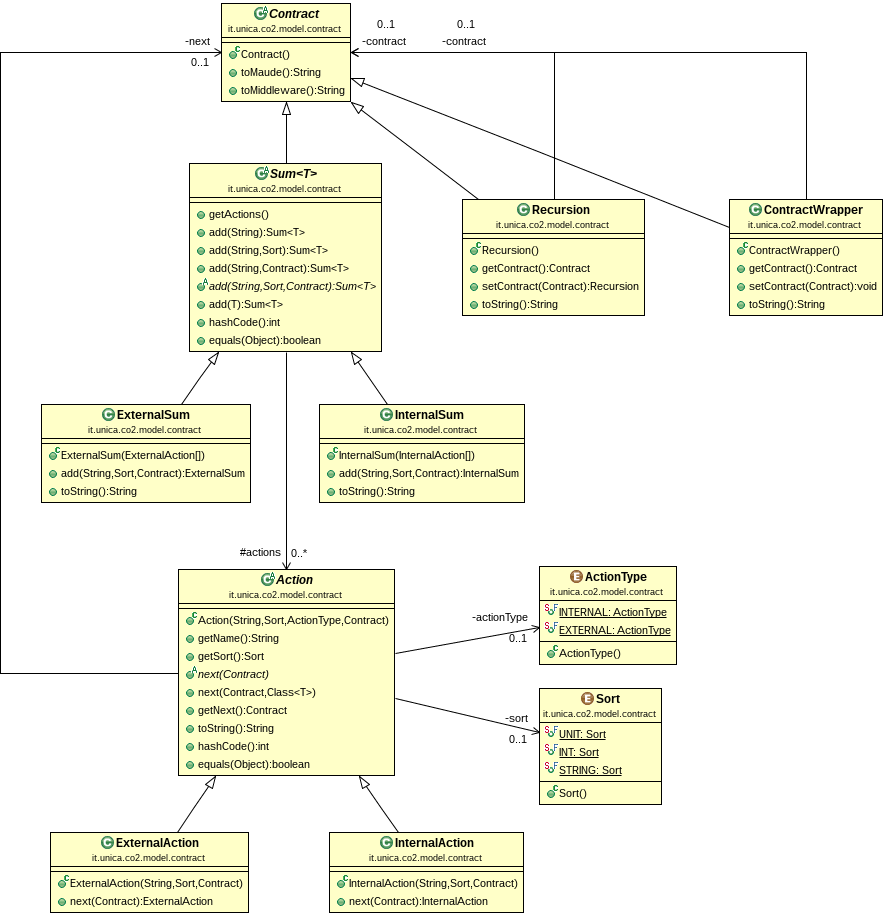
\includegraphics[scale=0.4]{img/class-diag/contracts.png}
	\caption{Class diagram of contracts}
	\label{fig:class-diag-contracts}
\end{figure}

\Cref{fig:class-diag-contracts} shows the class diagram of contracts. The \textit{abstract} class \incodeType{Contract} provides two utility methods, \incodeMethod{toMaude()} and \incodeMethod{toMiddleware()} that return the \incodeType{String} representation of the contract respectively in Maude syntax (needed for the honesty check) and timed session-types syntax (without the time guards).

\incodeType{Contract} is extended by the abstract class \incodeType{Sum}\generic[Action]{T} and the concrete classes \incodeType{Recursion} and \incodeType{ContractWrapper}. 

The \incodeType{Sum} is extended by \incodeType{ExternalSum}\generic{ExternalAction} and \incodeType{InternalSum}\generic{InternalAction}, that respectively represent the \textit{external} and \textit{internal choices} described in \Cref{def:contracts:syntax}.
The simplest way to construct a sum is shown in \Cref{lst:contract-sum}: the overloaded method \incodeType{Sum}\generic{T}.\incodeMethod{add(...)} allows to add an action \incodeType{T}, specifies its \incodeType{Sort}, and sets the next contract. %Remember that session-types (\Cref{def:contracts:syntax}) not allow to define a \textit{sequence} directly, although you can obtain it with a chain of ``single-action'' sums.
%
%\begin{listing}
%	\inputJavaLineos{code/ex-contract-sum.txt}
%	\caption{Example of contract sums.}
%	\label{lst:contract-sum}
%\end{listing}

The  \incodeType{Recursion} and \incodeType{ContractWrapper} are substantially identical but with different semantics: a \incodeType{Recursion} is used to define \textit{recursive behaviour}, while the \incodeType{ContractWrapper} was introduced as a workaround to the Java restriction that (properly) one cannot refer to a variable not yet initialized. The latter has become necessary on automated code-generation (explained in \Cref{sec:co2-plugin}). 

An example of a recursive contract is shown in \Cref{lst:contract-rec}, where \incode{R} and \incode{C} represent the same contract (if \incode{R} is expanded, we obtain \incode{C}): at line \lineno{6} we set \incode{R} as the \textit{next} contract of \incodeKeyword{a} (\incode{R} is still undefined); at line \lineno{7} we set \incode{C} as the body of \incode{R}. The contract are represented by session-types, $\contr{R} = \rec{X}{ \atomOut{a} \contrSeq X \sumInt \atomOut{b} }$ while $\contr{C} = \atomOut{a} \contrSeq \rec{X}{(\atomOut{a} \contrSeq X \sumInt \atomOut{b})} \sumInt \atomOut{b}$.
%
%\begin{listing}
%	\inputJavaLineos{code/ex-contract-rec.txt}%
%	\caption{Example of recursive contract.}
%	\label{lst:contract-rec}
%\end{listing}



\subsection{Prefixes}
\coco prefixes are modelled in Java as method calls. These methods are defined mainly into two classes, \incodeType{Session2} %\generic[ContractModel]{T}
 and \incodeType{Participant}. The former provides those prefixes that require a \textit{fused} session, \ie send/receive; the latter simplifies the advertisement of a \incodeType{Contract} and the establishment of a session with another participant.

\subsubsection{Participant}
The abstract class \incodeType{Participant} models a \coco agent $\sys{\pmv{A}}{\procP}$ and provides some methods that simplify the usage of middleware API and are necessary to analyze the code with JPF. This methods are:
%
\begin{description}
	\item[\incodeMethod{tell(\incodeType{Contract})} : \incodeType{Public}] \hfill \\
	Tells the given contract and returns a \incodeType{Public} without waiting for a session. Corresponds to the \coco prefix $\tell {} {\freeze x \contrP}$.
%
	\item[\incodeMethod{tellAndWait(\incodeType{Contract})} : \incodeType{Session2}] \hfill \\
	Tells the given contract and waits until a session is fused. Corresponds to the \coco prefix $\tell {} {\freeze x \contrP} \cocoSeq \ask{x}{true}$.
%	
	\item[\incodeMethod{waitForSession(\incodeType{Public})} : \incodeType{Session2}] \hfill \\
	Blocks the execution until a session is fused and assumes you already invoke \incodeMethod{tell(\incodeType{Contract})}. Corresponds to the \coco prefix $\ask{x}{true}$.
%	
	\item[\incodeMethod{waitForSession(\incodeType{Public},\incodeType{Integer})} : \incodeType{Session2}] \hfill \\
	As above, but specifying a timeout and throwing an exception if it expires. Corresponds to the \coco prefix $\ask{x}{true} \cocoPlus \tau$.
\end{description}

%\begin{figure}
%	\centering
%	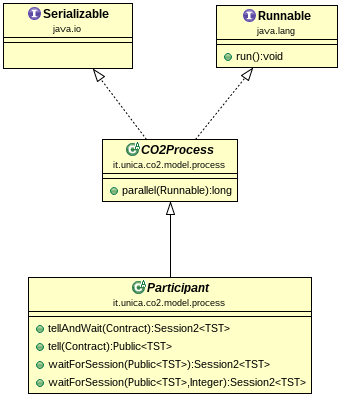
\includegraphics[scale=0.5]{img/class-diag/co2-processes.png}
%	\caption{Class diagram of precesses}
%	\label{fig:class-diag-processes}
%\end{figure}


%\begin{listing}[hp]
%	\inputJavaLineos{code/ex-process-participant.txt}
%	\caption{Example of a participant.}
%	\label{lst:process-participant}
%\end{listing}

The \incodeType{Participant} class extends the  \incodeType{CO2Process}, which implements the interfaces \incodeType{Serializable} (required by JPF) and \incodeType{Runnable}. The \incodeMethod{run()} method defines the ``behaviour'' of the process.
\Cref{lst:process-participant} shows a simple complete participant implementation.
%

\subsection{Parallel process}
\coco parallel processes are implemented as Java \incodeType{Thread}s and this explains the runnable nature of a participant. In fact the \incodeType{CO2Process} provides the following method:
%
\begin{description}
	\item[\incodeMethod{parallel(\incodeType{Runnable})} : \incodeType{long}] \hfill \\
	It starts a new \incodeType{Thread} that executes the given \incodeType{Runnable} object and returns the id of the thread.
\end{description}
%

%\begin{listing}
%	\inputJavaLineos{code/ex-process-parallel.txt}
%	\caption{Example of a parallel process.}
%	\label{lst:process-parallel}
%\end{listing}


In Java 8, you can invoke it taking advantage \textit{lambda expressions}. \Cref{lst:process-parallel} show you a process that take use of the parallel construct.


\subsection{Session}

The class \incodeType{Session} %\generic[ContractModel]{T}
(provided by the middleware API) lacks of some useful methods. A desirable method is \incodeMethod{waitForReceive(\incodeType{\incodeType{String\dots}\;\incodeBlack{actions}})} that takes as parameters the actions you want to receive: it waits until one of the specified actions is received.

Moreover, \incodeType{Session} does not provide a unique identifier, which would simplify the JPF analysis.
Therefore we extends it with the class \incodeType{Session2}, %\generic[ContractModel]{T}
whose most important methods are:
%
\begin{description}
	\item[\incodeMethod{waitForReceive(\incodeType{String\dots}\;\incodeBlack{actions})}]\label{item:session-wait} \hfill \\
	Corresponds to a sum of receive, \eg $\fact x {\atomIn{a}} \cocoPlus	\fact x {\atomIn{b}} \cocoPlus \fact x {\atomIn{c}}$.
	
	\item[\incodeMethod{waitForReceive(\incodeType{Integer} \incodeBlack{timeout,} \incodeType{String\dots}\;\incodeBlack{actions})}]\label{item:session-wait-timeout} \hfill \\
	Corresponds to a sum of receive with the timeout branch, \eg $\fact x {\atomIn{a}} \cocoPlus	\fact x {\atomIn{b}} \cocoPlus \fact x {\atomIn{c}} \cocoPlus \tau$.
	
	\item[\incodeMethod{send(\incodeType{String} \incodeBlack{action})}] \hfill \\
	This method corresponds to \coco the prefix $\fact x {\atomOut{a}}$.
	
	\item[\incodeMethod{send(\incodeType{String} \incodeBlack{action,} \incodeType{Integer} \incodeBlack{value})}] \hfill \\
	This method corresponds to \coco the prefix $\fact x {\atomOut{a}} e$ with $e$ of sort $\sort{int}$.
	
	\item[\incodeMethod{send(\incodeType{String} \incodeBlack{action,} \incodeType{String} \incodeBlack{value})}] \hfill \\
	This method corresponds to \coco the prefix $\fact x {\atomOut{a}} e$ with $e$ of sort $\sort{string}$.
	
\end{description}


%\begin{figure}
%	\centering
%	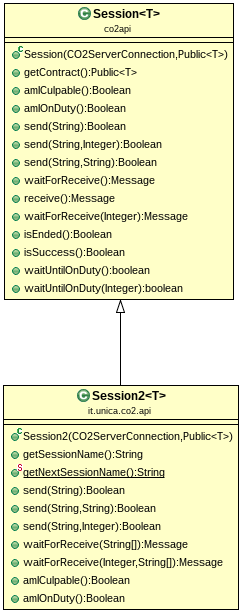
\includegraphics[scale=0.5]{img/class-diag/session2.png}
%	\caption{Class diagram of sessions}
%	\label{fig:class-diag-session2}
%\end{figure}


\subsection{Untranslatable code}\label{sec:untranslatable-code}
Not all \coco processes can be translated to Java code, due to language limits or the lack of sense. For example consider the non-deterministic choice of the sum process: the semantics (\Cref{fig:co2:semantics}) states that any prefix can be \textit{consumed} if permitted by the \textit{contract configuration}. 

In Java, we do not trace contract configuration changes, so there is no way to translate sums without losing the semantics, except for these ones that contain input prefixes (\eg $\fact x {\atomIn{a}} \cocoPlus \fact x {\atomIn{b}}$ or $\fact x {\atomIn{a}} \cocoPlus	\fact x {\atomIn{b}} \cocoPlus \tau$), in which the branch is chosen based on an external input. Even in this case, we can translate only sums of actions of the same type.
Now consider the process $\fact x {\atomOut{a}} \cocoPlus	\fact x {\atomOut{b}} \cocoPlus \fact x {\atomOut{c}}$: at first glance, you can be tempted to use the \incodeType{Random} class to make a choice and fire an output. However, this approach is not correct because the choice is made without considering the contract configuration and the corresponding \coco process would be $\tau \cocoSeq \fact x {\atomOut{a}} \cocoPlus	\tau \cocoSeq \fact x {\atomOut{b}} \cocoPlus \tau \cocoSeq \fact x {\atomOut{c}}$, whose meaning is different by the first one.

Furthermore we cannot translate processes if the $\ask{}{}$ prefix is missed before the use of a session. This limitations is now related to the fact that a session must be explicitly requested to the middleware. %For the same reason, we cannot pass a session as an actual parameter if is not preceded by an $\ask{}{}$.


\section{\coco Eclipse plugin}\label{sec:co2-plugin}

The \coco Eclipse plugin is implemented with Xtext, a framework for development of programming languages and \textit{Domain Specific Languages} (DSL) (\Cref{sec:xtext}), which moreover is part of the Eclipse ecosystem and maintained as an official project. The correct way of define our plugin would be \textit{Xtext plugin}: in fact we create an Xtext project, which provides all the scaffolding classes needed to add special functionality like code validation, syntax highlighting, etc.

\subsection{Grammar definition}

We define the \coco grammar using the Xtext DSL. Since the generated parser is LL(*), it is simple to write a grammar that fulfils the \coco specifications (although we must careful to not abuse of \textit{backtracking} due to performance reasons). The basic idea is that each rule corresponds to a Java class (instantiated when building the AST) and each declaration inside a rule is mapped to a class field. The implemented Xtext grammars are shown on \Cref{appchap:xtext-grammars}, categorized by type.

%\inputCocoFloat[h]{code/co2/sample.co2}{Example of \coco system}{lst:co2-sample}

\Cref{lst:co2-sample} is an example of a \coco process you can write with the plugin:
%
\begin{description}
	\item[\textnormal{Line \lineno{1}}] \hfill \\
	declares the system fully qualified name, used to generate \textit{target files} when the code will be translated to Maude and Java syntax.
	%
	\item[\textnormal{Line \lineno{3}}] \hfill \\
	specifies the main process that is considered for the honesty check (you can omit the whole line).
	%
	\item[\textnormal{Lines \lineno{5} and \lineno{9}}] \hfill   \\
	declare two contracts in which the former (a single-element external sum) is composed of the latter (an internal sum). Internal and external sums are respectively formed as  
	\incode{a1!} \incodeKeyword{T} \incode{+} \incode{a2!} \incodeKeyword{T}  \incode{+} \incode{aN!} \incodeKeyword{T} and 
	\incode{a1?} \incodeKeyword{T} \incode{(+)} \incode{a2?} \incodeKeyword{T}  \incode{(+)} \incode{aN?} \incodeKeyword{T}, where \incodeKeyword{T} can be \inlineCoco{int}, \inlineCoco{string} and \inlineCoco{unit} (in this case can be omitted).
	%
	\item[\textnormal{Lines \lineno{13} and \lineno{17}}] \hfill \\
	define the two processes \incode{P} and \incode{P1}.	
	Process \incode{P} declares a \textit{freename} of type \inlineCoco{session}, tell the contract \incode{C} and waits until the session \incode{y} is fused. Next, it waits for the action \incode{value}, storing the received value into the variable \incode{n} of type \inlineCoco{int}. Finally calls \incode{P1} with actual parameters \incode{n} and \incode{y}.	
	Process \incode{P1} takes the value \incode{n} and the session \incode{x}, next sends the action \incode{greater} if \incode{n>0}, \incode{lower} otherwise.
%
\end{description}

The keyword \inlineCoco{nil} defines an empty contract/process. The supported sorts are \inlineCoco{int}, \inlineCoco{string} and \inlineCoco{unit} for the declaration of actions into contracts, and \inlineCoco{int}, \inlineCoco{string}, \inlineCoco{boolean} and \inlineCoco{session} for the declaration of freenames.

\Cref{chap:use-cases} contains more complicated examples showing the completeness of the grammar.

\subsection{Scoping}
The scope of a name binding is the part of the program where the binding is valid. Xtext provides an out-of-the-box scoping system that can be customized to fit particular requirements. 

\subsubsection{Contracts}
Contracts contain two type of references, one to another contract and one to a recursion definition. The former is resolved between all contracts definition in the same file, except the one containing the reference, while the latter is resolved between all recursions defined into the same contract and \emph{before} the reference.

\Cref{lst:co2-contract-scope} shows an example of scoping. \incode{C1} is a recursive contract, \incode{C2} and \incode{C3} are two semantically equivalent contracts, but the scope of \incode{A} is limited to \incode{C1} so \incode{C2} does not compile.
Also \incode{C1} and \incode{C4} are semantically equivalent, but the visibility of \incode{C4} is hidden within \incode{C4} itself.
%
This behaviour is a little bit cumbersome and error prone: to avoid problems, you must use the \inlineCoco{rec} construct to define \textit{recursive behaviour} and use references between contracts only for \textit{composition} (manually avoiding loops). The scoping rules try to mitigate this problem, but these ones can be bypassed as shown in \Cref{lst:co2-contract-infinite}. This problem will be resolved in the future.

%\inputCocoFloat{code/co2/contracts-scope.co2}{Example of contract scoping}{lst:co2-contract-scope}

%\inputCocoFloat{code/co2/contracts-infinite.co2}{Example of infinite contract loop}{lst:co2-contract-infinite}

\subsubsection{Processes}
Processes can contain references to contracts and to other processes, allowing composition and recursive behaviour. Both contracts and processes references are resolved among all the declarations inside the same file.



\subsection{Validation}
Custom validations were added according to \coco language specification. The validation phase occurs after the parsing and linking phases, covered automatically by Xtext based on the grammar definition and the scoping customization.

The validation phase covers not only errors reporting, but warnings and info too. Consider for example if a freename declaration hides another one, maybe without changing its type: the process is correct (respecting the syntax and the static typing), but can lead to an unexpected behaviour if you do not see the freename you're hiding, so we report a warning.

Implemented validations are:
\begin{description}\itemsep0pt

	\item[\error{error}:] uniqueness of process names on declarations
	
	\item[\error{error}:] uniqueness of contract names on declarations
	
	\item[\error{error}:] the \inlineCoco{honesty} keyword must be followed by a process reference that takes no arguments

	\item[\error{error}:] action names inside a contract sums must be unique, \ie neither \inlineCoco{a! (+) a!} nor \inlineCoco{a? + a?} are permitted
	
	\item[\warning{warning}:] freenames shadowing (including recursion names)
	
	\item[\info{info}:] the \inlineCoco{unit} action type can be omitted
	
	\item[\info{info}:] the \inlineCoco{nil} keyword, representing empty contracts and  processes, can be omitted
	
\end{description}

\subsubsection{Type system}
The \coco type system is implemented using Xsemantics, a DSL (implemented in Xtext itself) for writing type systems, reduction rules, interpreters (and in general relation rules) for languages implemented in Xtext.

Into our grammar, \textit{freenames} can be declared and used in different places (see \Cref{appsec:xtext-co2} for details). The declaration of a freename can occur in a formal parameter, in a delimited process or in a input prefix: any type can be used among \inlineCoco{int}, \inlineCoco{string}, \inlineCoco{boolean} and \inlineCoco{session} when declaring a formal parameter or a delimited process, while input variables are limited to \inlineCoco{int} and \inlineCoco{string} type.

Referred freenames can be used inside an expressions, except for the \inlineCoco{session} type. Furthermore, we check the match between the actual and formal parameters types on process invocation.

%\begin{listing}
%	\inputJavaLineos{code/xtext/sample.xsemantics}
%	\caption{Part of the type-system rules}
%	\label{lst:xsemantics-sample}
%\end{listing}

Into practice, we implement a set of \textit{rules} whose result (a Java type) depends on a set of \textit{premises}. Rules without premises are \textit{axioms}. Considering this aspect, is possible to write potentially any validation rule using the Xsemantics engine. \Cref{lst:xsemantics-sample} shows some simple rules and we refer to \Cref{appsec:xsemantics} for the full implementation.


\subsection{Code generation}
The plugin can automatically transform from \coco syntax to Maude and Java languages.
The code generation happens navigating the AST and translating each \coco construct to the corresponding code of the target language. The Maude representation of \coco is complete, so it is always possible to obtain a translation and verify the honesty of the process using \cite{verifiable}, as explained in \Cref{sec:maude:checker}. On the other hand, as focused in \Cref{sec:untranslatable-code}, not all processes can be translated to Java.

The \inlineCoco{system} declaration is used to produce the target files, \eg \inlineCoco{system} \inlineCoco{com.example.co2.Sample} will produces \textit{Sample.maude} and \textit{Sample.java} inside the directory structure \texttt{/com/example/co2/Sample}.

A complete example of auto-generated code can be found in \Cref{chap:use-cases}.
%
\section{The Java honesty checker}\label{sec:java-honesty}

This chapter covers the problem of verifying the honesty of Java applications.
To achieve this goal, \textit{Java PathFinder} (JPF, discussed in \Cref{sec:jpf}) is used to analyze the Java bytecode and to build up the agent $\sys{\pmv{A}}{\procP}$, represented as a Java object.
After this building phase, the honesty of the process must be checked in some way: in order to reuse other related work on \coco, the Maude model-checker described in \Cref{sec:maude:checker} is used to verify the honesty.

Note: in this chapter the term \textit{process} is used as the abbreviation of \coco process.

\section{Construction phase}\label{sec:construction-phase}
The building phase is incrementally explained in this section, so we start from a single thread application with neither composition nor recursion, ending to a composed (maybe recursive) program that can launch multiple parallel threads.

As described in \Cref{sec:jpf}, JPF allows to define a \emph{listener} that can handle multiple events meanwhile the $\text{JVM}_{JPF}$ explores all possible states of our program. 

We handle the execution of some specific methods, object creations and bytecode instructions.

\subsubsection{Handled methods}
The handled methods signatures are:
\begin{description}
	
	\item[\incodeType{Participant}.\incodeMethod{tell(\incodeType{Contract})} : \incodeType{Public}] \hfill \\
	It tells the given contract and immediately returns. You can get a session using the returned \incodeType{Public} object. It corresponds to the \coco prefix $\tell {} {\freeze x \contrP}$.
	
	\item[\incodeType{Participant}.\incodeMethod{tellAndWait(\incodeType{Contract})} : \incodeType{Session2}] \hfill \\
	It tells the given contract and waits until the session starts. It is a shortcut for \incodeMethod{waitForSession(\incodeMethod{tell(\incodeType{Contract})})}. It corresponds to $\tell {} {\freeze x \contrP} \cocoSeq \ask{x}{true}$.
	
	\item[\incodeType{Participant}.\incodeMethod{waitForSession(\incodeType{Public})} : \incodeType{Session2}] \hfill \\
	It waits until a session starts. It corresponds to $\ask{x}{true}$.

	\item[\incodeType{Participant}.\incodeMethod{waitForSession(\incodeType{Integer},\incodeType{Public})} : \incodeType{Session2}] \hfill \\
	It waits until a session starts, throwing a \incodeType{TimeExpiredException} if the timeout expires. It corresponds to $\ask{x}{true} \cocoPlus \tau$.
	
	\item[\incodeType{Session2}.\incodeMethod{send(\incodeType{String})} : \incodeKeyword{void}] \hfill \\
	It sends the specified action without a value. It corresponds to $\fact x {\atomOut{a}}$.

	\item[\incodeType{Session2}.\incodeMethod{send(\incodeType{String}, \incodeType{String})} : \incodeKeyword{void}] \hfill \\
	It sends the specified action with a string value. It corresponds to $\fact x {\atomOut{a}} e$ with $e$ of sort $\sort{int}$.
	
	\item[\incodeType{Session2}.\incodeMethod{send(\incodeType{String}, \incodeType{Integer})} : \incodeKeyword{void}] \hfill \\
	It sends the specified action with a integer value. It corresponds to $\fact x {\atomOut{a}} e$ with $e$ of sort $\sort{string}$.
	
	\item[\incodeType{Session2}.\incodeMethod{waitForReceive(\incodeType{String\dots})} : \incodeType{Message}] \hfill \\
	It waits until any of the given actions is received. It corresponds to a sum of receives, \eg $\fact x {\atomIn{a}} \cocoPlus	\fact x {\atomIn{b}} \cocoPlus \fact x {\atomIn{c}}$. Note that all actions must be of the same type.
	
	\item[\incodeType{Session2}.\incodeMethod{waitForReceive(\incodeType{Integer}, \incodeType{String\dots})} : \incodeType{Message}]\hfill \\
	As above, throwing a \incodeType{TimeExpiredException} if the given timeout expires. It corresponds to a sum of receive with the timeout branch, \eg $\fact x {\atomIn{a}} \cocoPlus	\fact x {\atomIn{b}} \cocoPlus \fact x {\atomIn{c}} \cocoPlus \tau$. Note that all actions must be of the same type.
	
	\item[\incodeType{Participant}.\incodeMethod{parallel(\incodeType{Runnable})} : \incodeKeyword{long}] \hfill \\
	It starts a new thread that will execute the given runnable object. The corresponding \coco process is better explained in \Cref{sec:java-parallel}.
	
	\item[\incodeType{Participant}.\incodeMethod{<init>} \textnormal{and} \incodeType{CO2Process}.\incodeMethod{<init>}]  \hfill \\
	They respectively construct a \incodeType{Participant} and a \incodeType{CO2Process}. These constructors are handled to allow process composition.
	
	\item[\incodeType{Participant}.\incodeMethod{run()} \textnormal{and} \incodeType{CO2Process}.\incodeMethod{run()}]  \hfill \\
	We catch the entrance (exit) to (from) a method in order to handle the process start (termination).
\end{description}

\subsubsection{If statement}
We also handle the bytecode instructions involving in the \textit{if-then-else} statement. By default, JPF would evaluate the \textit{if condition} and execute only the corresponding branch. We customize this behaviour, exploring both branches to build up the \coco process $\ifte{\expE}{\procP}{\procP}$.


\subsection{Single process}
This section covers the simplest building, \ie a single process with neither compositions nor spawning of parallel processes. The idea is that each method listed above creates a new \incodeType{ProcessDS} (\eg \incodeType{SumDS}, \incodeType{IfThenElseDS}, etc.) in which can be appended one or more \incodeType{PrefixDS} (\eg \incodeType{TauDS}, \incodeType{TellDS}, etc.). The full implementation of \incode{*DS} classes, used to model \coco precesses, is shown in \Cref{appchap:java-honesty} (\textit{DS} states for \textit{Data Structure}).

Consider a Java program that executes these lines of code:

\begin{mdframed}
\begin{minted}[fontsize=\footnotesize,linenos]{java}
Contract c = ...;
Public p = tell(c);
Session session = waitForSession(p);

session.send("a");
session.waitForReceive("b", "c");

session.send("d");
\end{minted}
\end{mdframed}

First of all, we need to trace: the \textit{current process}, that is the \coco main process we are building up; the \textit{current prefix}, that is the \coco prefix in which we append the next process. When a method invocation is handled,
\begin{inlinelist}
	\item we create a new process that represents it,
	\item we append it to the current prefix (if it is the first invocation, we simply set the current process) and
	\item we set/override the current prefix.
\end{inlinelist}

Considering the example above, the construction takes place in this way:
\begin{description}
	\item[Line \lineno{2}:] \hfill \\
	new process: $\tell {} {\freeze x \contrP}$ \hfill(single-element sum)\\
	current process: $\tell {} {\freeze x \contrP}$ \hfill(single-element sum)\\
	current prefix: $\tell {} {\freeze x \contrP}$
	
	\item[Line \lineno{3}:] \hfill \\
	new process: $\ask{x}{true}$ \hfill(single-element sum)\\
	current process: $\tell {} {\freeze x \contrP} \cocoSeq \ask{x}{true}$\\
	current prefix: $\ask{x}{true}$
	
	\item[Line \lineno{5}:] \hfill \\
	new process: $\fact x {\atomOut{a}}$ \hfill(single-element sum)\\
	current process: $\tell {} {\freeze x \contrP} \cocoSeq \ask{x}{true} \cocoSeq \fact x {\atomOut{a}}$\\
	current prefix: $\fact x {\atomOut{a}}$
	
	\item[Line \lineno{6}:] \hfill \\
	new process: $\fact x {\atomIn{b}} \cocoPlus \fact x {\atomIn{c}}$\\
	current process: $\tell {} {\freeze x \contrP} \cocoSeq \ask{x}{true} \cocoSeq \fact x {\atomOut{a}} \cocoSeq \fact x {\atomIn{b}} \cocoPlus \fact x {\atomIn{c}}$\\
	current prefix: $unknown$
\end{description}

The current prefix at line \lineno{6} is unknown when invoking the \incodeMethod{waitForReceive} method, because it depends on the input received from the participant involved in the session. At this point JPF comes into play: the method returns if the action \incodeKeyword{b} or \incodeKeyword{c} is received, so we instruct JPF to explore all possible choices and it automatically take care of state advancing and backtracking when reaches the end of a branch.
Continuing the construction, we have now two states:

\begin{description}
	
	\item[State 1:] the action \incodeKeyword{b} is received. The current prefix is set to $\fact x {\atomIn{b}}$.
	\begin{description}
		\item[Line \lineno{6}:] \hfill \\
		new process: $\fact x {\atomIn{b}} \cocoPlus \fact x {\atomIn{c}}$\\
		current process: $\tell {} {\freeze x \contrP} \cocoSeq \ask{x}{true} \cocoSeq \fact x {\atomOut{a}} \cocoSeq \fact x {\atomIn{b}} \cocoPlus \fact x {\atomIn{c}}$\\
		current prefix: $\fact x {\atomIn{b}}$
		
		\item[Line \lineno{8}:] \hfill \\
		new process: $\fact x {\atomOut{d}}$ \hfill(single-element sum)\\
		current process: $\tell {} {\freeze x \contrP} \cocoSeq \ask{x}{true} \cocoSeq \fact x {\atomOut{a}} \cocoSeq ( \fact x {\atomIn{b}} \cocoSeq \fact x {\atomOut{d}} \cocoPlus \fact x {\atomIn{c}} )$\\
		current prefix: $\fact x {\atomOut{d}}$\\
		\textbf{Note:} the construction ends (no further code) and JPF backtracks.
	\end{description}	
	
	\item[State 2:] the action \incodeKeyword{c} is received. The current prefix is set to $\fact x {\atomIn{c}}$.	
	\begin{description}
		\item[Line \lineno{6}:] \hfill \\
		new process: $\fact x {\atomIn{b}} \cocoPlus \fact x {\atomIn{c}}$\\
		current process: $\tell {} {\freeze x \contrP} \cocoSeq \ask{x}{true} \cocoSeq \fact x {\atomOut{a}} \cocoSeq ( \fact x {\atomIn{b}} \cocoSeq \fact x {\atomOut{d}} \cocoPlus \fact x {\atomIn{c}} )$\\
		current prefix: $\fact x {\atomIn{c}}$\\
		\textbf{Note:} the current process is the result of the exploration of the first state.
		
		\item[Line \lineno{8}:] \hfill \\
		current process: $\tell {} {\freeze x \contrP} \cocoSeq \ask{x}{true} \cocoSeq \fact x {\atomOut{a}} \cocoSeq ( \fact x {\atomIn{b}} \cocoSeq \fact x {\atomOut{d}} \cocoPlus \fact x {\atomIn{c}} \cocoSeq \fact x {\atomOut{d}} )$\\
		current prefix: $\fact x {\atomOut{d}}$\\
		\textbf{Note:} the construction ends (no further code) and there are not other states to be explored.
	\end{description}
\end{description}

The construction is terminated and the complete \coco process is
\[
\tell {} {\freeze x \contrP} \cocoSeq \ask{x}{true} \cocoSeq \fact x {\atomOut{a}} \cocoSeq ( \fact x {\atomIn{b}} \cocoSeq \fact x {\atomOut{d}} \cocoPlus \fact x {\atomIn{c}} \cocoSeq \fact x {\atomOut{d}} )
\]

The constructs that create new states are:
\begin{itemize}
	\item \textit{if-then-else}: generates two states, one for each branch;
	
	\item \incodeMethod{waitForReceive(..)}: generates one state for each action (and an additional state if you specify a timeout);
	
	\item \incodeMethod{waitForSession(\incodeBlack{timeout})}: generates two states, one in case the session is fused and one if the timeout expires. Note: the \incodeMethod{waitForSession()} without a timeout does not generate new states.
\end{itemize}

\subsubsection{Conclusion}
When JPF backtracks from a state to another one, we must set the correct current prefix, otherwise the new process will be wrongly appended somewhere else. To achieve this goal we must save the \textit{new process} before starting the exploration of a new state, \eg $\fact x {\atomIn{b}} \cocoPlus \fact x {\atomIn{c}}$ in the example above. Storing it in a variable is not enough because another construct could generate other states that will override it. The solution is to adopt a \emph{stack} and read from the top when we need to retrieve the correct value to set the \textit{current prefix}.

Summing up, the following data structures are required to build a single process:
\begin{inlinelist}
	\item the \textit{current process},
	\item the \textit{current prefix} and
	\item a stack to store the \textit{new process} when multiple states were generated (henceforth referred as \textit{choices stack})
\end{inlinelist}

\subsection{Process composition}\label{sec:java-process-composition}
Process composition allows not only to write more readable processes but also to define a \textit{recursive behaviour}, like
\[ 
\contr{c} \mmdef \rec{\contrX}{\atomOut{a}\contrSeq \contrX \sumInt \atomOut{b}}
\]
\[
\procP \; = \; (x) \; \tell {} {\contr{c}} \cocoSeq \procX(x) \hspace{30pt}\procX(x) \mmdef \ifte{\expE}{\fact x {\atomOut{a}} \cocoSeq \procX(x) }{ \fact x {\atomOut{b} }}
\]

In Java, it is equivalent to define a new class that extends \incodeType{CO2Process} (or \incodeType{Participant} if you need to get a new session), create a new instance and invoke its \incodeMethod{run()} method. We catch the creation of the new instance and save the left side of the definition (\eg $\procX(x)$) carrying about the formal parameters declaration. When this instance starts (entering the method \incodeMethod{run()}) the building of the current process suspends and the new one begin. On finished, the invoking process must be restored so its built phase can continue. Note although that it is not possible to append other prefixes to a process invocation (since the \coco does not permit it), but it could be the end part of a branch, as shown in \Cref{lst:if-build-example}

%%%%%\begin{listing}
%	\inputJavaLineos{code/jpf/if-build-composition.java}
%	\caption{Example of process composition into a \textit{if} statement}
%	\label{lst:if-build-example}
%\end{listing}


Under these conditions, it is necessary to use a \emph{stack} to save the data structures listed at the end of the previous section, henceforth referred as \textit{\coco{}Stack} and \textit{\coco{}StackFrame} respectively. When a process starts, a new frame is allocated onto the stack and used to build up the corresponding \coco process; once it terminates, the frame is removed. In order to obtain the full graph of invocations, the callee process takes a reference to the called one, and at the end of the day it is possible to reach each process by starting from the main one.

\subsubsection{Recursion}
Now it is possible to define recursive processes. The problem is that $\text{JVM}_{JPF}$ would concretely execute each process call, so it could throw a \textit{stack-overflow exception} when trying to build our \coco process. At first glance, you could think that if the recursion is \textit{under control} (\ie providing a stop condition) then there will be no problems. However, we must explore all branches of if-statements, so this approach does not work.

The idea is to detect the recursion and break method call: on \incodeMethod{run()} method invocation, before pushing the \textit{\coco{}StackFrame} onto the stack, we check that it does not contain a frame for the same process. In this way, the recursion is detected and the exploration can stop safely.
Note that this strategy can lead to unexpected behaviour at runtime if you do not provide a stop condition.

%\begin{listing}
%	\inputJavaLineos{code/jpf/rec-build-composition.java}
%	\caption{Example of recursive process calls}
%	\label{lst:rec-build-example}
%\end{listing}

\Cref{lst:rec-build-example} shows a Java recursive application. The corresponding \coco process will be

\[
	\begin{array}{rcl}
		\procP & \; = \;& (x)\; \tell {} {\freeze x \contrP} \cocoSeq \ask{x}{true} \cocoSeq \procPi(x)
	\\
	\procPi(x) & \; \mmdef \;& \fact x {\atomOut{a}} \cocoSeq \procPii(x)
	\\
	\procPii(x) & \; \mmdef \;& \fact x {\atomIn{b}} \cocoSeq \procPi(x)
	\end{array}
\]	

\subsection{Parallel processes}\label{sec:java-parallel}
The \coco parallel process maps directly to a Java \incodeType{Thread}, which is executed asynchronously with the callee. We use the method \incodeMethod{parallel(\incodeType{Runnable})} in order to handle its invocation and the start of the new thread. The method is \emph{synchonized}, so there are not overlaps due for example to multiple threads that try to start a parallel process. In this way, when handling the call with JPF, we are sure to make the correct association between the caller and the callee thread.

The execution is now more complicated due to the scheduling of the spawn threads. Fortunately JPF allows to retrieve the thread identifier when handling the method calls, so we extend our data structure using a map of $\langle thread\, ID, \coco{}Stack\rangle$. When a new thread starts, it is linked to the caller and each of them construct its \coco process independently from the other one.  

\subsubsection{Example}
The example below shows how the \coco process is built by a Java application that spawn new threads.

\begin{mdframed}
\begin{minted}[fontsize=\footnotesize,linenos]{java}
//some code A

parallel(()->{
    //some code B
});

parallel(()->{
    //some code C
});

//some code D
\end{minted}
\end{mdframed}

The description is trivial: some code $A$ is executed, then a new thread executes $B$ asynchronously, another one executes $C$, finally the main thread continues with $D$.

The construction is made as follow:

\begin{description}
	\item[Line \lineno{1}:] \hfill \\
	current process: $\procFmt{A}$\\
	current prefix: the last prefix added to $\procFmt{A}$
	
	\item[Line \lineno{3}:] \hfill \\
	new process: $(\,\tau_{m1} \,|\, \tau_1\,)$\\
	current process (main thread): $\procFmt{A} \cocoSeq (\,\tau_{m1}\, | \,\tau_1\,)$\\
	current prefix (main thread): $\tau_{m1}$ \\
	current process (thread-1): $\tau_1$ \hspace{30pt}(single-element sum)\\
	current prefix (thread-1): $\tau_1$ \\
	\textbf{Note:} the construction of the process of thread-1 starts immediately.
	
	\item[Line \lineno{7}:] \hfill \\
	new process: $(\,\tau_{m2}\, | \,\tau_2\,)$\\
	current process (main thread): $\procFmt{A} \cocoSeq (\,\tau_{m1} \cocoSeq (\,\tau_{m2} \,|\, \tau_2\,) \,| \,\tau_1\,)$\\
	current prefix (main thread): $\tau_{m2}$ \\
	current process (thread-2): $\tau_2$ \hspace{30pt}(single-element sum)\\
	current prefix (thread-2): $\tau_2$ \\
	\textbf{Note:} the construction of the process of thread-2 starts immediately.
	
	\item[Line \lineno{9}:] \hfill \\
	new process: $\procFmt{D}$\\
	current process (main thread): $\procFmt{A} \cocoSeq (\,\tau_{m1} \cocoSeq (\,\tau_{m2} \cocoSeq \procFmt{D}  \,|\, \tau_2\,) \,| \,\tau_1\,)$\\
	
	\item[Line \lineno{4}:] \hfill \\
	new process: $\procFmt{B}$\\
	current process (thread-1): $\tau_1 \cocoSeq \procFmt{B}$\\
	
	\item[Line \lineno{8}:] \hfill \\
	new process: $\procFmt{C}$\\
	current process (thread-2): $\tau_2 \cocoSeq \procFmt{C}$\\
	
\end{description}

When the construction is finished, the first \textit{\coco{}Frame} of the main process contains the \coco process
\[
		\procP \; = \; \procFmt{A} \cocoSeq (\,\tau \cocoSeq (\,\tau \cocoSeq \procFmt{D}  \,|\, \tau \cocoSeq \procFmt{C}\,) \,| \,\tau \cocoSeq \procFmt{B}\,) \equiv \procFmt{A} \cocoSeq (\, \procFmt{B} \,|\, \procFmt{C}\, | \,\procFmt{D}\,)
\]

\subsubsection{Construction flaws}
Unfortunately, we do not care about the actions types. This originates from the impossibility to specify the contract actions types to the middleware and it is not related to other limitations.

\section{Verification phase}\label{sec:verification-phase}
The previous section describes how a \coco process is reconstructed from a Java program. This process is modelled into classes (\Cref{appchap:java-honesty}) and can be checked for honesty. In order to reuse other related works on \coco, we decide to serialize it as a Maude program and model-check it as described in \Cref{sec:maude:checker}. If the reconstruction is correct, we ensure that the Java program is honest and probably will not fail at runtime.

\section{Honesty verification}
Putting together the phases explained above, from a given \incodeType{Participant} we can build the corresponding \coco process exploring all significant states and verify its honesty. \incodeType{HonestyChecker.}\incodeMethod{isHonest()} is the provided method that allows to do so, whose input is \incodeType{Class}\generic[Participant]{?} and returns an enumeration of \incodeType{HONEST}, \incodeType{DISHONEST} or \incodeType{UNKNOWN} (the latter in order to cover unexpected errors occurs).


% \printbibliography[heading=bibintoc]

\bibliographystyle{abbrv}
\bibliography{main}

\end{document}